\documentclass[dvipdfmx, titlepage, t]{jsarticle}

% \usepackage{geometry}
\usepackage[dvipdfmx]{graphicx}
\usepackage{ascmac}
\usepackage{amsmath}
\usepackage{amssymb}
\usepackage{minted}
\usepackage{listings}
% \usepackage[utf8]{inputenc}
% \usepackage{listingsutf8}
\usepackage{newfloat} % newfloat パッケージを読み込む
\usepackage{caption}
\usepackage{float}
\usepackage{fix-cm}
\usepackage{svg}
\usepackage{enumitem}

\usepackage{hyperref}
% for hyperref
\usepackage{pxjahyper}
\hypersetup{
    dvipdfmx,
	colorlinks=false, % リンクに色をつけない設定
	bookmarks=true, % 以下ブックマークに関する設定
	bookmarksnumbered=true,
	pdfborder={0 0 0},
	bookmarkstype=toc
}

% \lstset{
%   basicstyle={\ttfamily},
%   identifierstyle={\small},
%   inputencoding=auto,
%   commentstyle={\small\sffamily},
%   keywordstyle={\small\bfseries},
%   ndkeywordstyle={\small},
%   stringstyle={\small\ttfamily},
%   frame={tb},
%   breaklines=true,
%   columns=[l]{fullflexible},
%   numbers=left,
%   % xrightmargin=0zw,
%   % xleftmargin=3zw,
%   numberstyle={\scriptsize},
%   firstnumber=auto,
%   stepnumber=1,
%   numbersep=5pt,
%   lineskip=1ex
% }

% 新しい浮動体「listing」を定義
\DeclareFloatingEnvironment[
    fileext=lol,       % List of Listings ファイルの拡張子 (List of Listings を作成する場合)
    name=Listing,      % キャプションの接頭辞 (例: "Listing 1")
    placement={!htbp}, % フロートの配置オプション (お好みで調整してください)
    within=section     % 番号付けをセクションごとにする場合 (例: Listing 1.1) (任意、不要なら削除)
]{program}

\setminted{
  mathescape,              % 数式モードへのエスケープを許可 (必要なら)
  % basicstyle やフォント関連
  fontsize=\small,         % 全体のフォントサイズ (listings の \small に合わせる試み)
                           % \ttfamily は minted のデフォルトに近いが、日本語対応の等幅フォントを
                           % LaTeX 側で \ normaalfont や \ttdefault に設定しておくのが理想
  % frame
  frame=lines,             % 上下に線を引く frame=tb に近いものとして lines (上下左右に線)
  framesep=2mm,            % 枠線とコードの間隔 (調整が必要)
  % breaklines
  breaklines=true,         % 自動折り返し
  % numbers
  linenos=true,            % 行番号を左に表示
  firstnumber=auto,        % 行番号を開始行に合わせる
  numbersep=5pt,           % 行番号とコードの間隔
  % stepnumber=1,          % linenos=true で通常1ステップ
  % highlight と Pygments スタイル
  % minted では Pygments のスタイルを使います。
  % style=friendly のようにスタイル名を指定できます。
  % デフォルトのスタイルでキーワードが太字になるか確認。
  % commentstyle や keywordstyle の LaTeX コマンド直接指定はできません。
  % Pygments のスタイルでこれらがどのように見えるか確認し、
  % 必要ならカスタムスタイルを作るか、別の既存スタイルを選びます。
}

\title{生体情報を用いた計測と分析}
\author{情報学群 \\ 1270328 佐藤謙成}
\date{\today}

\begin{document}
\maketitle

\begin{abstract}
    眼球運動計測では,高精度な Eye Link II を用いて顔画像の魅力度を判断する視線行動の解析を行い,Tobii Glass 3 では自然な状況下の視線と注視している部分を調べる.筋電計測では,上腕二頭筋の活動をMVCを基準に,異なるダンベル負荷で評価する.脳波計測では, P300 を用いてブレイン・マシン・インターフェースによる文字入力を行った.
\end{abstract}


\section{全体の目的}
\subsection{第六回の目的}
    第六回では,地球に到達する光を分析することにより,恒星の動きを知ることを目的とする.恒星がどの程度の速度で地球から遠ざかっているのかを算出し,観測されたスペクトルを描画する.また,複数の恒星を分析することでどのような関係性を持っているのかを明らかにする.

\subsection{第七回の目的}
    第七回では,次回の眼球運動計測実験の準備としてMatLab及びPsychotoolboxを用いてプログラムを作成する.正確なタイミング管理が必要な事件に向いている Psychotoolbox を用いる.また,本課題では被験者が左右に提示される顔画像の魅力を判断し,キー押しで反応する二者択一の選択課題を 2 試行行う実験環境を構築することである.
\subsection{第八回の目的}

\subsection{第九回の目的}
    第九回では,EyeLink II によって過去に測定された眼球運動実験のデータをプログラムを用いて解析することである.EyeLink II は,参加者のセットアップ,キャリアブレーション,検証が迅速かつ簡単に用いることができる.また,微細な眼球運動の解析やリアルタイムでのデータ処理にも適しているため用いる.目的としては,被験者が左右の顔画像のどちらかを選択する際に,選択した顔画像にどの程度視線を向けていたかの確率を時間経過とともにグラフ化することで視線がどのように動くのかを明らかにする.

\subsection{第十回の目的}
    第十回では,異なる負荷条件下で記録された筋電図データを解析し,各条件下での筋活動レベルを定量的に評価することで負荷と筋活動の関係を求めることである.

\section{方法}
\subsection{第六回の方法}
    \begin{program}
        \caption{データの読み込み}
        \inputminted[linenos, firstline=1, lastline=2, frame=lines, fontsize=\small]{matlab}{code/Exp3_6_Matlab.m}
        \label{lst:exp_3_6_load}
    \end{program}

    コード\ref{lst:exp_3_6_load} では,与えれらた starData というデータファイルを読み込み, size(spectra, 1) で描くスペクトルに含まれる観測点の亜k図を取得する.

    次に,恒星 HD94028 のスペクトルを抽出する.それが以下のコード \ref{lst:exp3_6_s}である.
    \inputminted[linenos, firstline=14, lastline=19, frame=lines, fontsize=\small]{matlab}{code/Exp3_6_Matlab.m}
    ここでは,データの値が非常に広範囲に渡っているため,両軸対数スケールで出力するために関数 loglog を用いている.また,恒星 HD94028 のスペクトルはベクトル s に格納する.

    ベクトル s に格納された値を用いて水素アルファ線の波長を求める.コード \ref{lst:exp3_6_alpha} では, s の最小値が水素アルファ線であることを利用して \mintinline{matlab}|min(s)| で求めている.関数 min はここでは 2つの値を出力することができる.一つ目の値が水素アルファ線の値で二つ目の値がそのインデックスとなる.

    \inputminted[linenos, firstline=20, lastline=23, frame=lines, fontsize=\small]{matlab}{code/Exp3_6_Matlab.m}

    特定した水素アルファ線に対して点を追加するためのコードがコード\ref{lst:exp3_6_hold}である. ここでは, \mintinline{matlab}|hold on| を記述することで既存のグラフに点を追記することができ, \mintinline{matlab}|hold off| で追記を終了することができる.今回は,水素アルファ線の値の部分にマーカーサイズが 8 の赤い正方形をプロットする.
    \inputminted[linenos, firstline=24, lastline=27, frame=lines, fontsize=\small]{matlab}{code/Exp3_6_Matlab.m}
    
    赤方偏移係数と星が地球から遠ざかる速度を求める.赤方偏移係数は係数を $z$ としたときに $z = \dfrac{\lambda Ha }{656.28} - 1$ で求めることができるため,これを実装する.速度に関しては,赤方偏移係数に光速の値をかけることで求めることができる.
    \inputminted[linenos, firstline=29, lastline=31, frame=lines, fontsize=\small]{matlab}{code/Exp3_6_Matlab.m}

    % svgに変更しよう
    \begin{figure}[H]
        \centering
        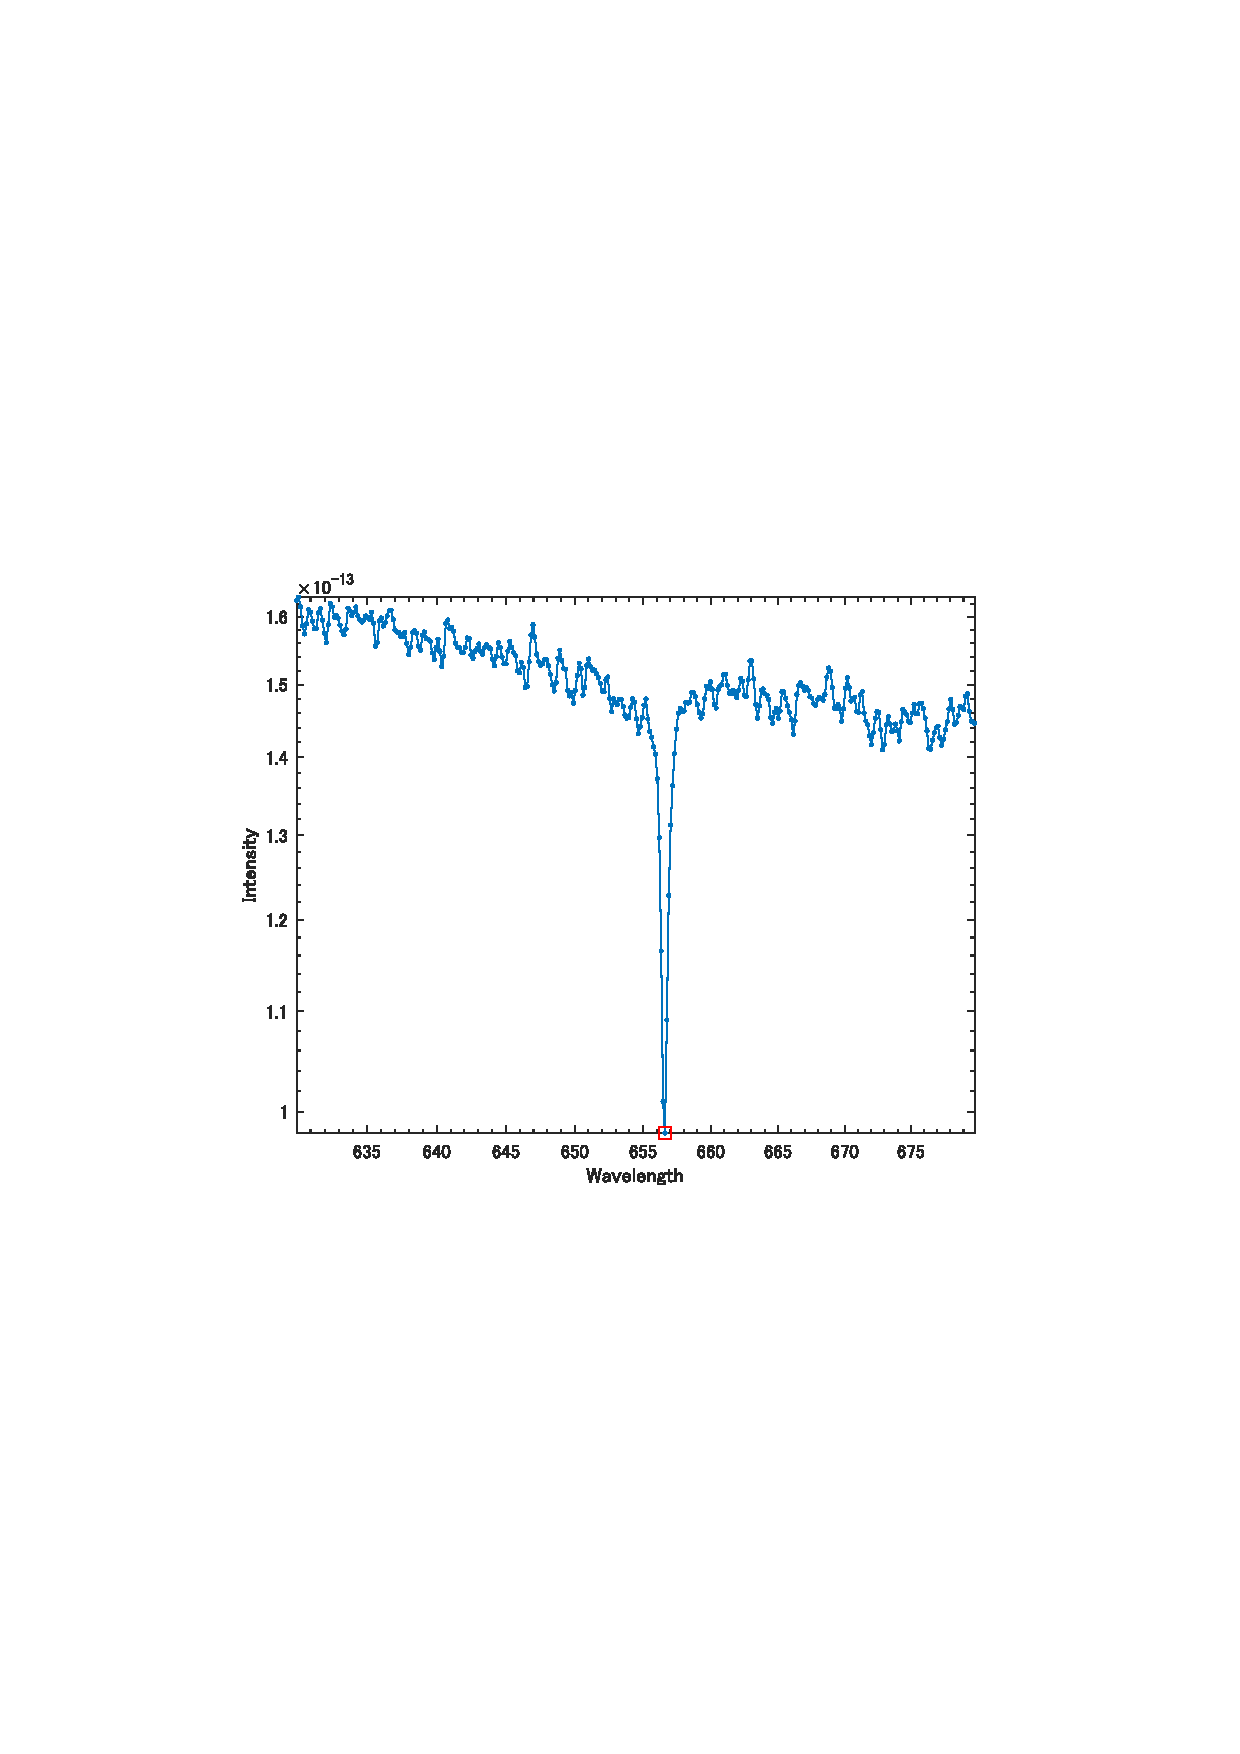
\includegraphics[width=0.5\textwidth]{figure/stellar1.pdf}
        \caption{恒星 HD94028 のスペクトルと水素アルファ線}
        \label{fig:exp3_6_spectra}
    \end{figure}

    ここから,各星の水素アルファ線を求める.行列の各行に対して最小値とそのインデックスを計算する.これは \mintinline{matlab}|min(spectra(:,:))| で求めることができる.また,各星の Ha の波長を \mintinline{matlab}|lambda(idx)|で求め,その値を用いて赤方偏移係数と速度を求める.

    \inputminted[linenos, firstline=11, lastline=15, frame=lines, fontsize=\small]{matlab}{code/Exp3_6_2_Matlab.m}

    この各星で求めた値を1つの図にまとめるプログラムで出力する.全ての星のスペクトルを一つのグラフに目止めて描画し,青方偏移か赤方偏移を視覚的に区別し,どの線がどの星に対応するかを明確にする.各星について速度が 0 以下の場合は青方偏移,0 より大きい場合は赤方偏移と判断するため,if文を用いて条件分岐を行う.また,その条件分岐を各星に対して行うために for 文を用いる.
    \inputminted[linenos, firstline=16, lastline=27, frame=lines, fontsize=\small]{matlab}{code/Exp3_6_2_Matlab.m}

    % svgに変更しよう
    \begin{figure}[H]
        \centering
        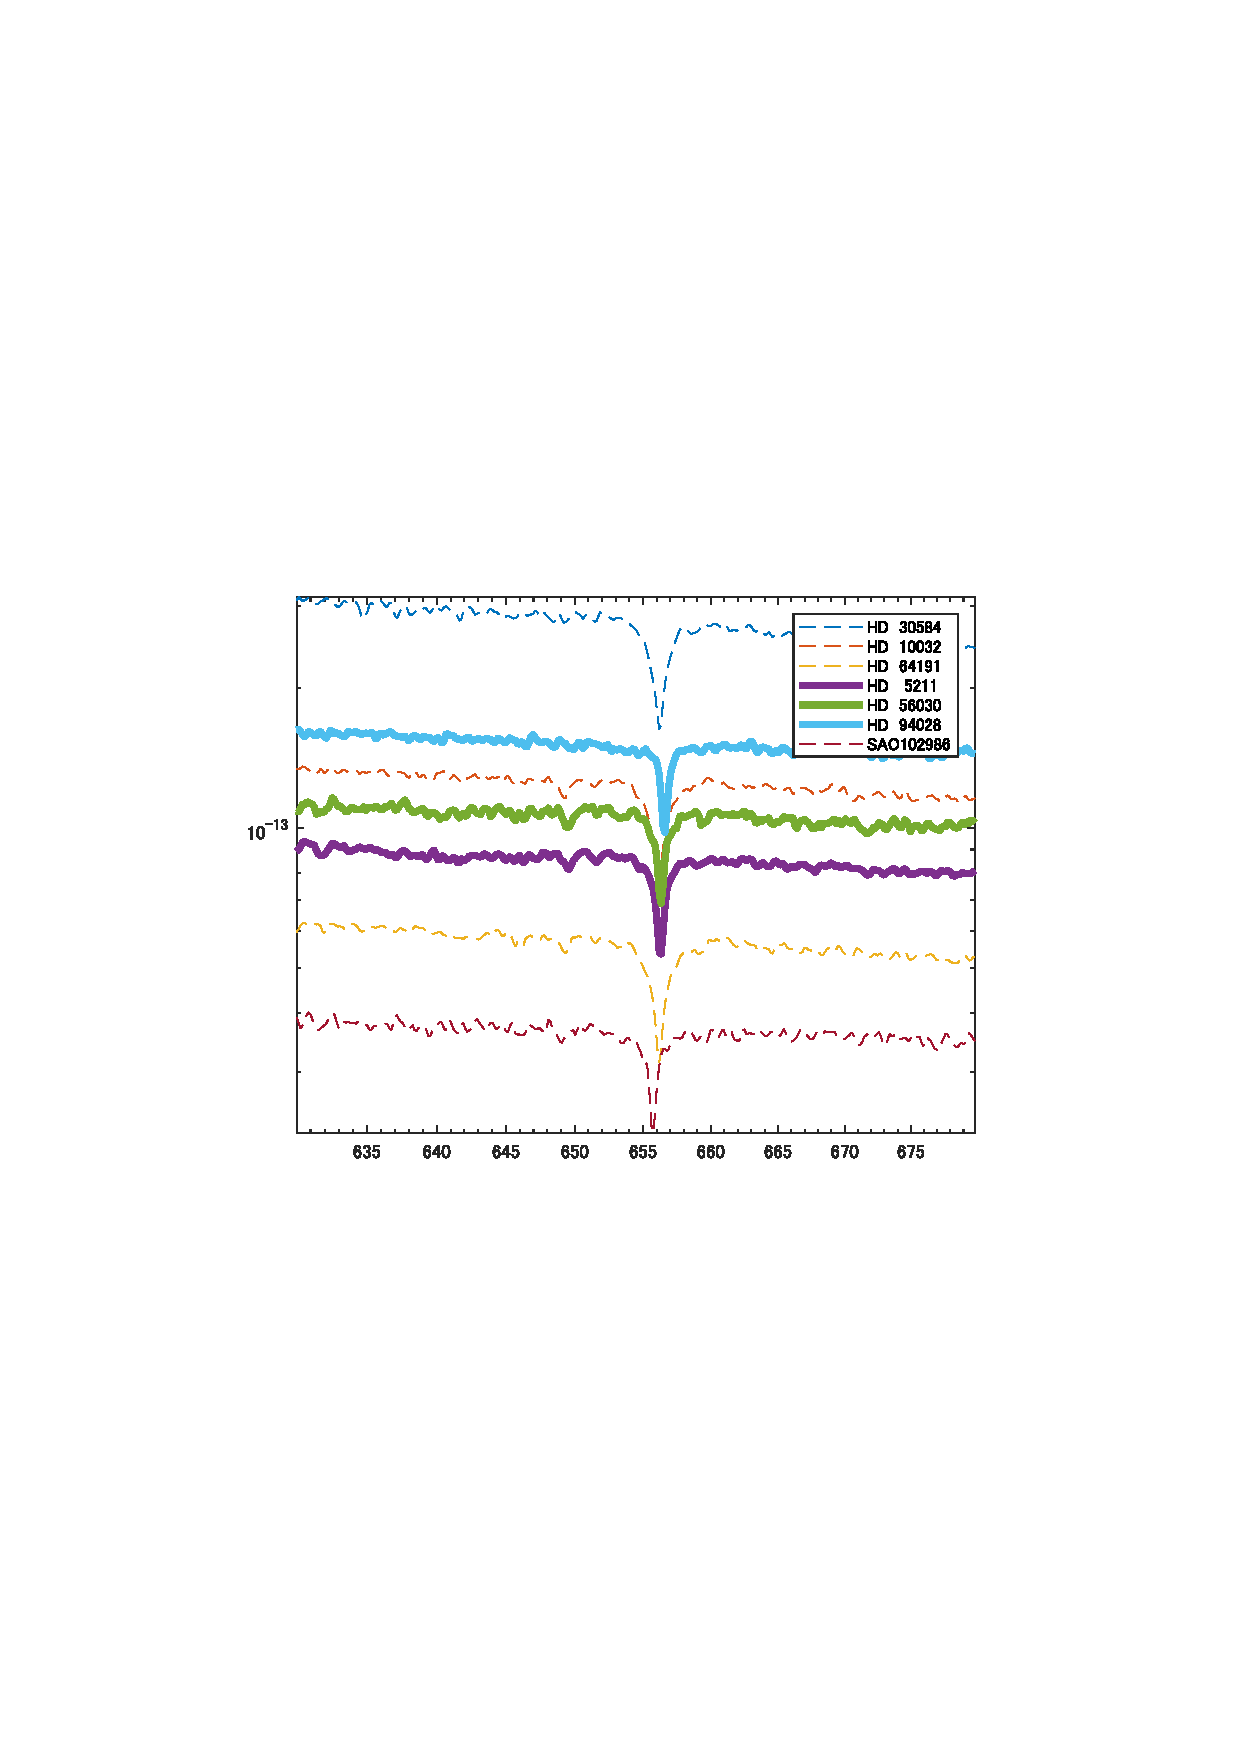
\includegraphics[width=0.5\textwidth]{figure/stellar2.pdf}
        \caption{各星のスペクトルと水素アルファ線}
        \label{fig:exp3_6_spectra2}
    \end{figure}

\subsection{第七回の方法}
    まず,刺激呈示環境を構築する.まず,背景色を白色とするために \mintinline{matlab}|bgcolor = 255| と設定する.刺激画像の大きさは 640 $\times$ 480 とする.今回提示する顔画像は与えられたデータを用いる.

    \begin{program}[H]
    \inputminted[linenos, firstline=5, lastline=12, frame=lines, fontsize=\small]{matlab}{code/Exp3_7_Matlab.m}
    \end{program}

    画面左右端と画像端との距離は 220 ピクセルとするため, \mintinline{matlab}|margin = 220| とする.固視点は 画像中央に幅 40,縦 4 及び 幅 4 縦 40 の黒色の十字とする.黒色は 0 で指定することができ,固視点の十字は長方形を二つで組み合わせることで表現できる.ここで長方形は \mintinline{matlab}|[left top right bottom]| でベクトルで定義できる.
    \begin{program}[H]
        \inputminted[linenos, firstline=32, lastline=36, frame=lines, fontsize=\small]{matlab}{code/Exp3_7_Matlab.m}      
        \caption{固視点の表示}
        \label{lst:exp3_7_eye}
    \end{program}

    固視点呈示後,準備された左右の顔画像を表示する.それはコード\ref{lst:exp3_7_window}で表示することができる.
    \begin{program}[H]
        \caption{刺激の呈示}
        \inputminted[linenos, 
        firstline=95,
        lastline=99,
        frame=lines,
        fontsize=\small]{matlab}{code/Exp3_7_Matlab.m}
        \label{lst:exp3_7_window}
    \end{program}

    刺激を呈示した後の回答を格納するための関数は \mintinline{matlab}|KbWait([], 3)| を用いる.KbWait の返り値の一つである keyCode1 で押されたキーが確認できるが 1 $\times$ 256 の論理配列であり,各キーに対応した要素を真である.keycode1 で真になった要素を探索するため関数 Find を使用して行った.そのコードが\ref{lst:exp3_7_get}である.今回使用するキーは g, j に制限する. 

    \begin{program}[H]
        \caption{反応時間の取得}
        \inputminted[linenos,
            firstline=102,
            lastline=107,
            frame=lines,
            fontsize = \small
        ]{matlab}{code/Exp3_7_Matlab.m}
        \label{lst:exp3_7_get}
    \end{program}

    これで,全ての試行が完了した後は,results配列にデータを格納するコードをコード\ref{lst:exp3_7_result}に示す.

    \begin{program}[H]
        \caption{データの保存}
        \inputminted[linenos,
        firstline=106,
        lastline=111,
        frame=lines,
        fontsize = \small]{matlab}{code/Exp3_7_Matlab.m}
        \label{lst:exp3_7_result}
    \end{program}

    最後に,results配列の値を csv ファイルに書き出した保存する.ここでは writematrix 関数を使用して \mintinline{matlab}| writematrix(results, filename)| と記述することで書き出すことができる.ここでの filename は,exp3\_7\_05.csv のことであり,拡張子に csv がついているため csv ファイルで保存される.
        \begin{program}[H]
        \caption{データの書き出し}
        \inputminted[linenos,
        firstline=129,
        lastline=132,
        frame=lines,
        fontsize = \small]{matlab}{code/Exp3_7_Matlab.m}
        \label{lst:exp3_7_write}
    \end{program}




    \subsection{第八回の方法}
    以下の 4 つの実験を行う.ただし,Eye Link II を用いる 眼球運動計測実験(1)については EyeLink II  が故障しているため,実施できなかった.
    \subsubsection{眼球運動計測実験 (1)}\label{眼球}
    時間計測度の高い眼球運動計測装置を用いて,顔の印象に関する判断を行う時に眼球運動の計測を行う.眼球運動計測装置として Eye Link II を用いる.EyeLink II は 画像\ref{fig:eye_link} である.まず,被験者に Eye Link II のカメラを装着し,キャリブレーション,バリデーションを行う.次に固視点を注視し,左右に現れる顔画像のどちらかが魅力的かを判断し,キー押しで反応してもらう.この試行を合計 20 試行行う.

    \begin{figure}[H]
        \centering
        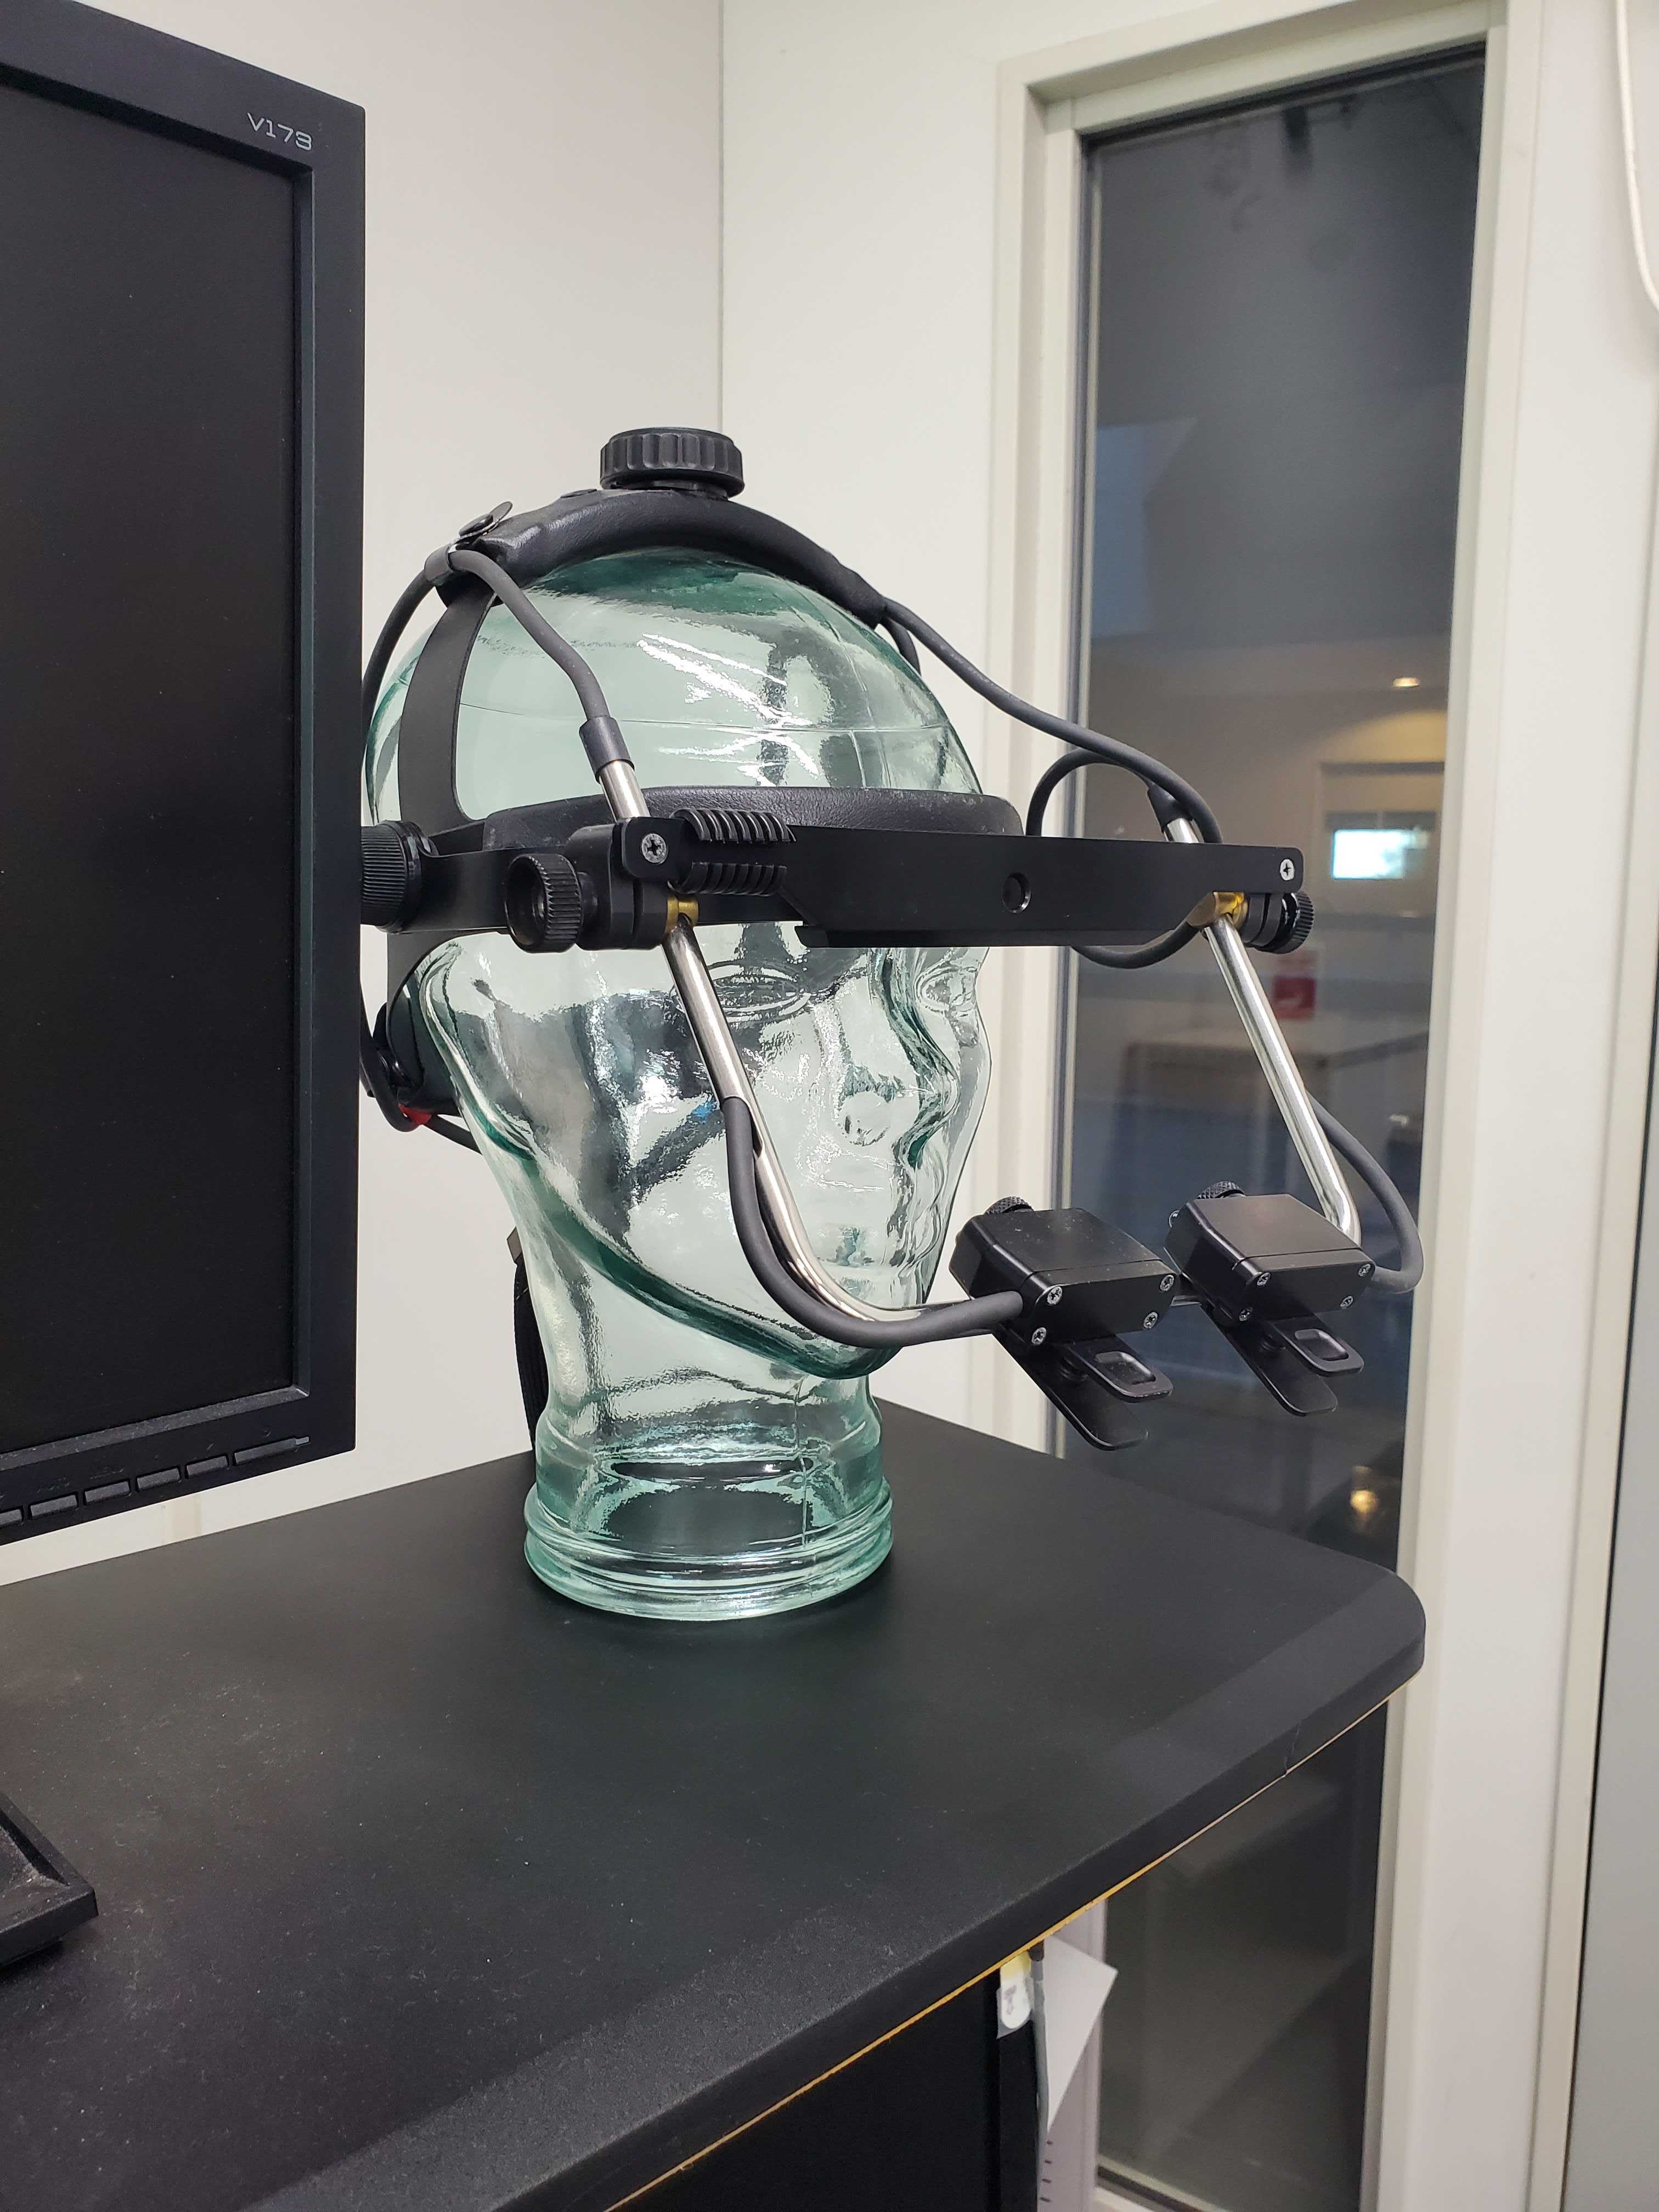
\includegraphics[keepaspectratio, width=0.6\linewidth]{figure/EyeLink.jpg}
        \caption{EyeLink II の画像}
        \label{fig:eye_link}
    \end{figure}

    \subsubsection{眼球運動計測実験 (2)}
    メガネ型眼球運動計測装置である Tobii Glass 3 を用いて対象を自由に見る時の眼球運動を解析する.実験の手続きとしてはアイトラッキング用メガネを装着し,呈示されるマーカを追視.視線方向のキャリブレーションを行う.ここで,対象を自由に観察した時の Gaze Plot と Heat Map を作成する.実際の実験風景は 画像\ref{fig:tobii} である.

    \begin{figure}[H]
        \centering
        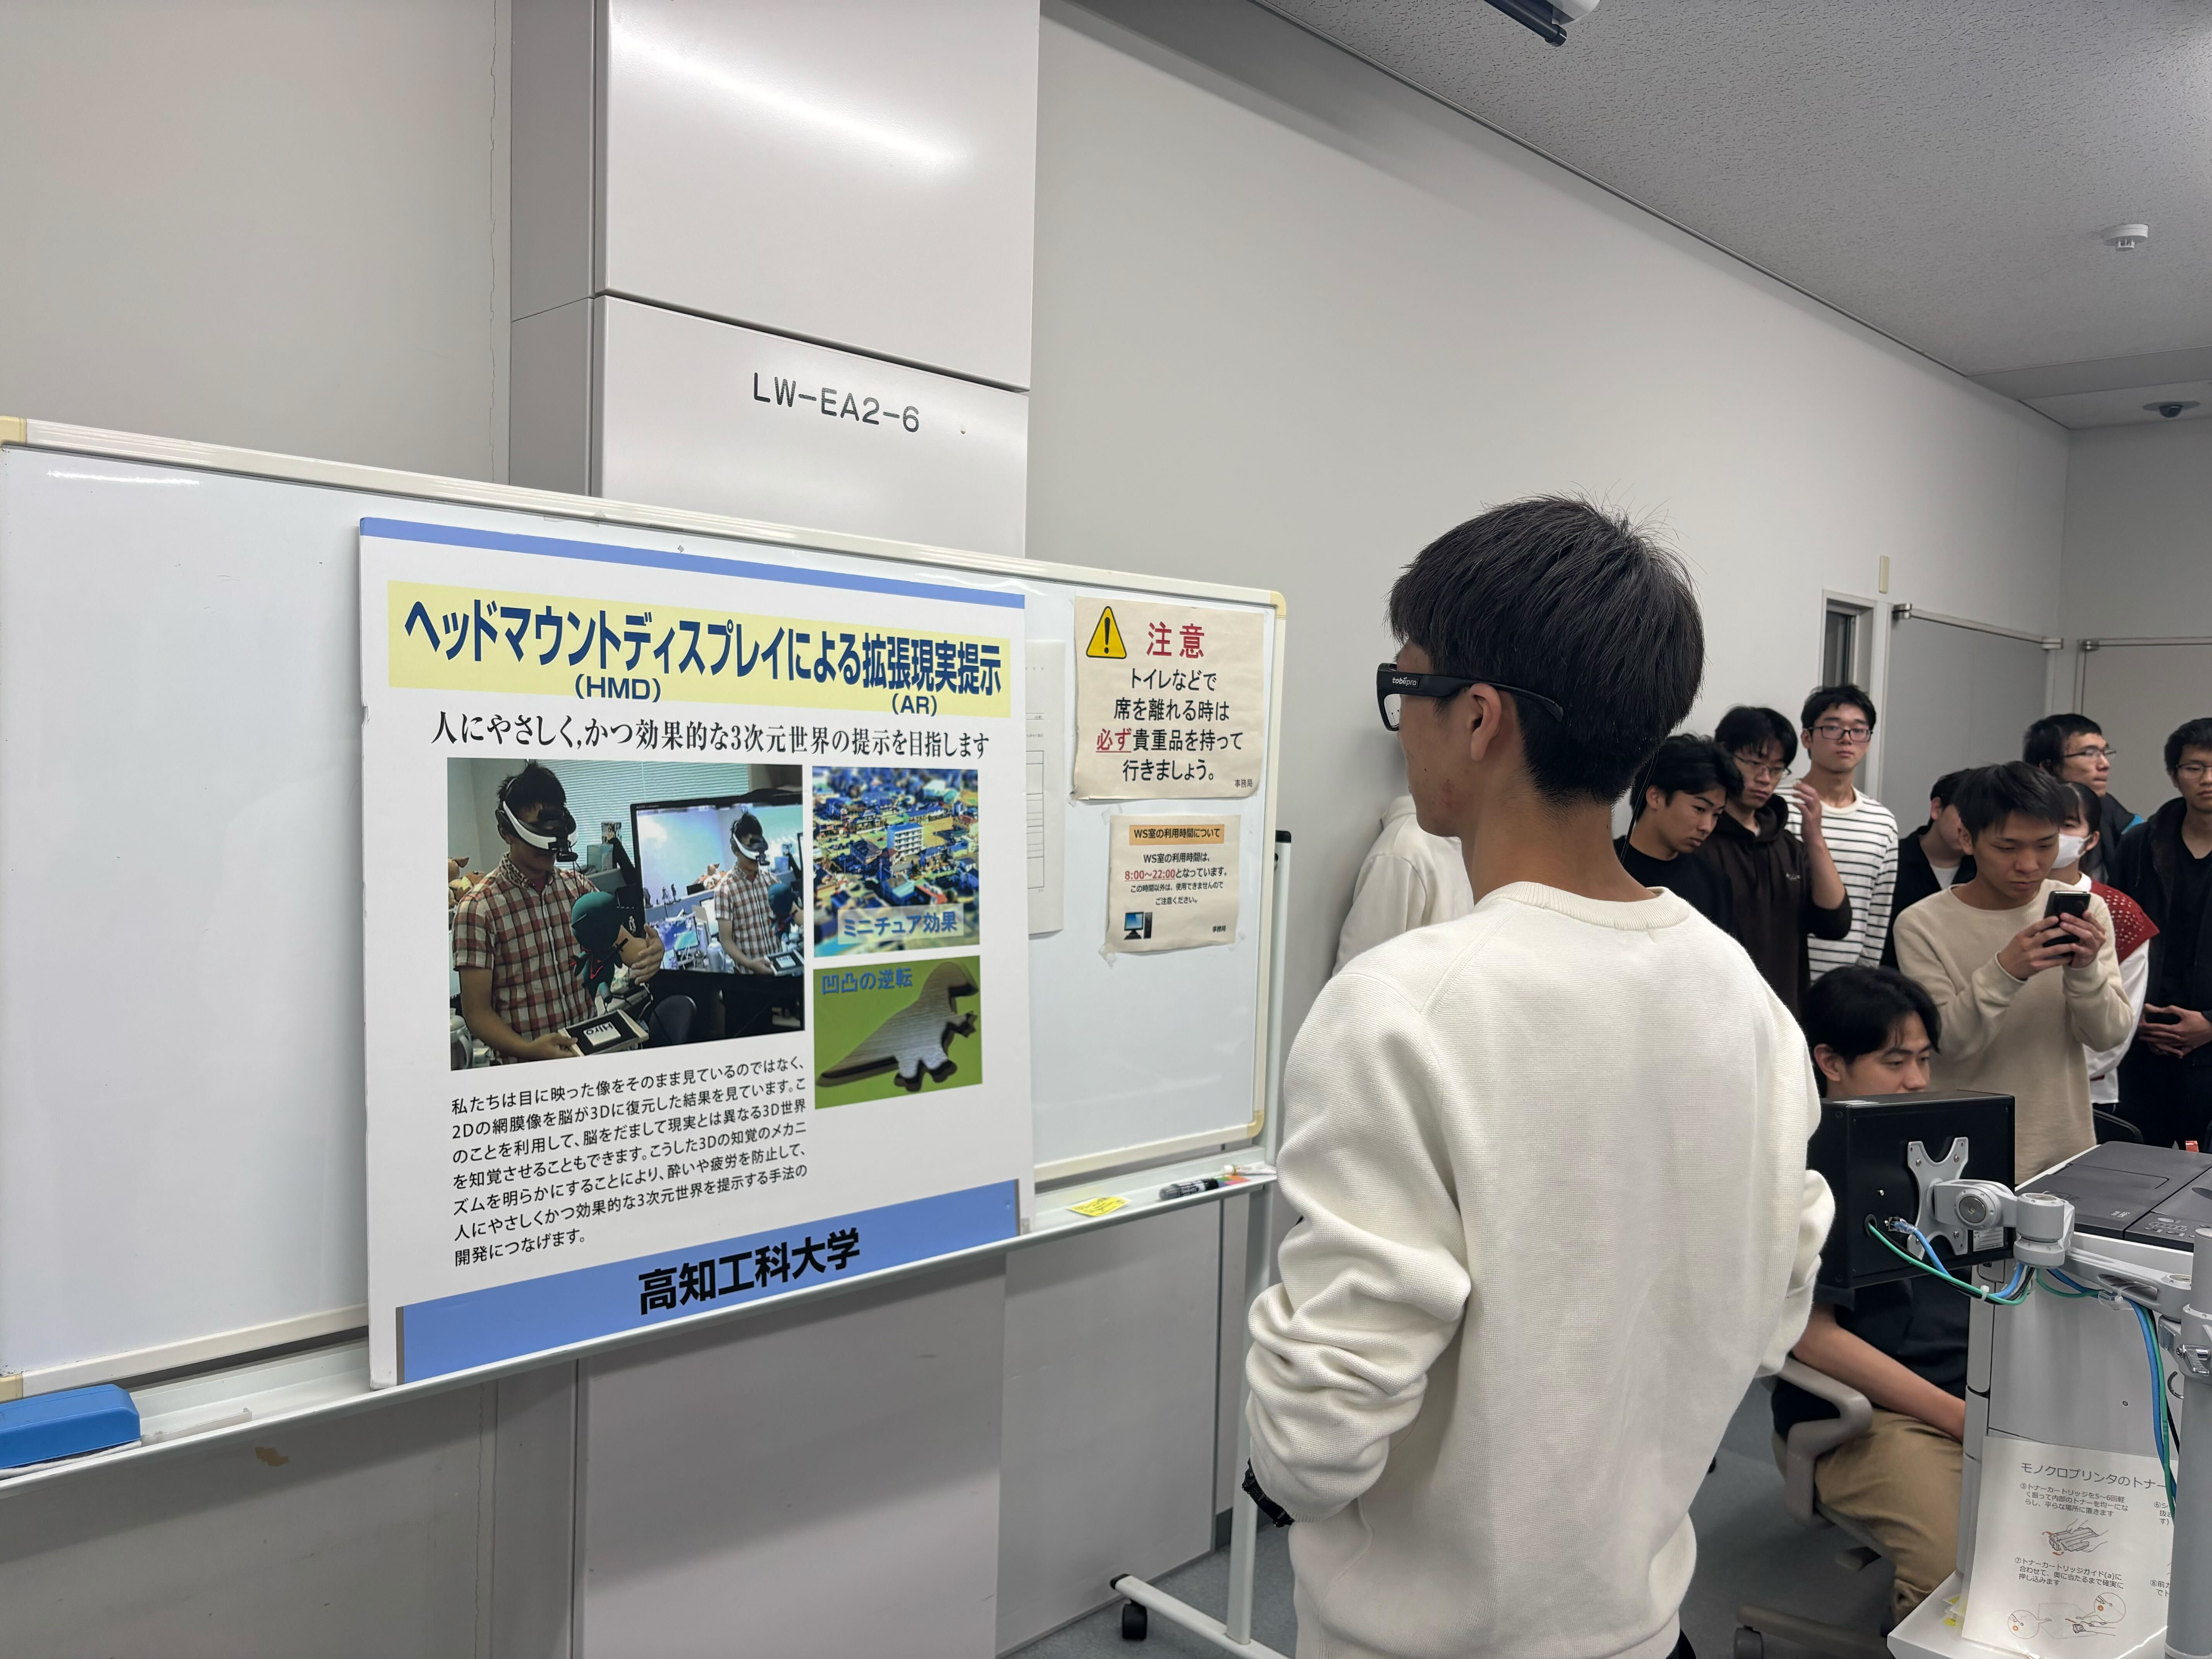
\includegraphics[keepaspectratio, width=0.6\linewidth]{figure/tobii.jpg}
        \caption{Tobii Glass 3 を用いた実験風景}
        \label{fig:tobii}
    \end{figure}

    \subsubsection{脳波計測}
    タイプしたい文字を脳情報のみから指定する非侵襲式ブレイン・マシン・インターフェースのシステムを体験する.被験者は PC 上に提示された $6 \times 6$ のマトリクスの文字を観察する.灰色の英字及び数字が黒の背景上に提示され,その中からランダムな順で 1 文字が 100ms だけ白色に変わる.その後,75ms はどの文字も灰色となり,別の文字が白くなる.脳波による指標は,刺激提示から約 300 ミリ秒ほど後に頂点をもって現れる陽性の脳電位である p 300 を用いる. MatLab から Simulink のブロックセットを起動する.ドライ電極を頭部に装着する.電極位置は電波キャップに従って決める.本実験では視覚的刺激を提示する.実際の実験風景は 画像\ref{fig:keisoku} である.

    \begin{figure}[H]
        \centering
        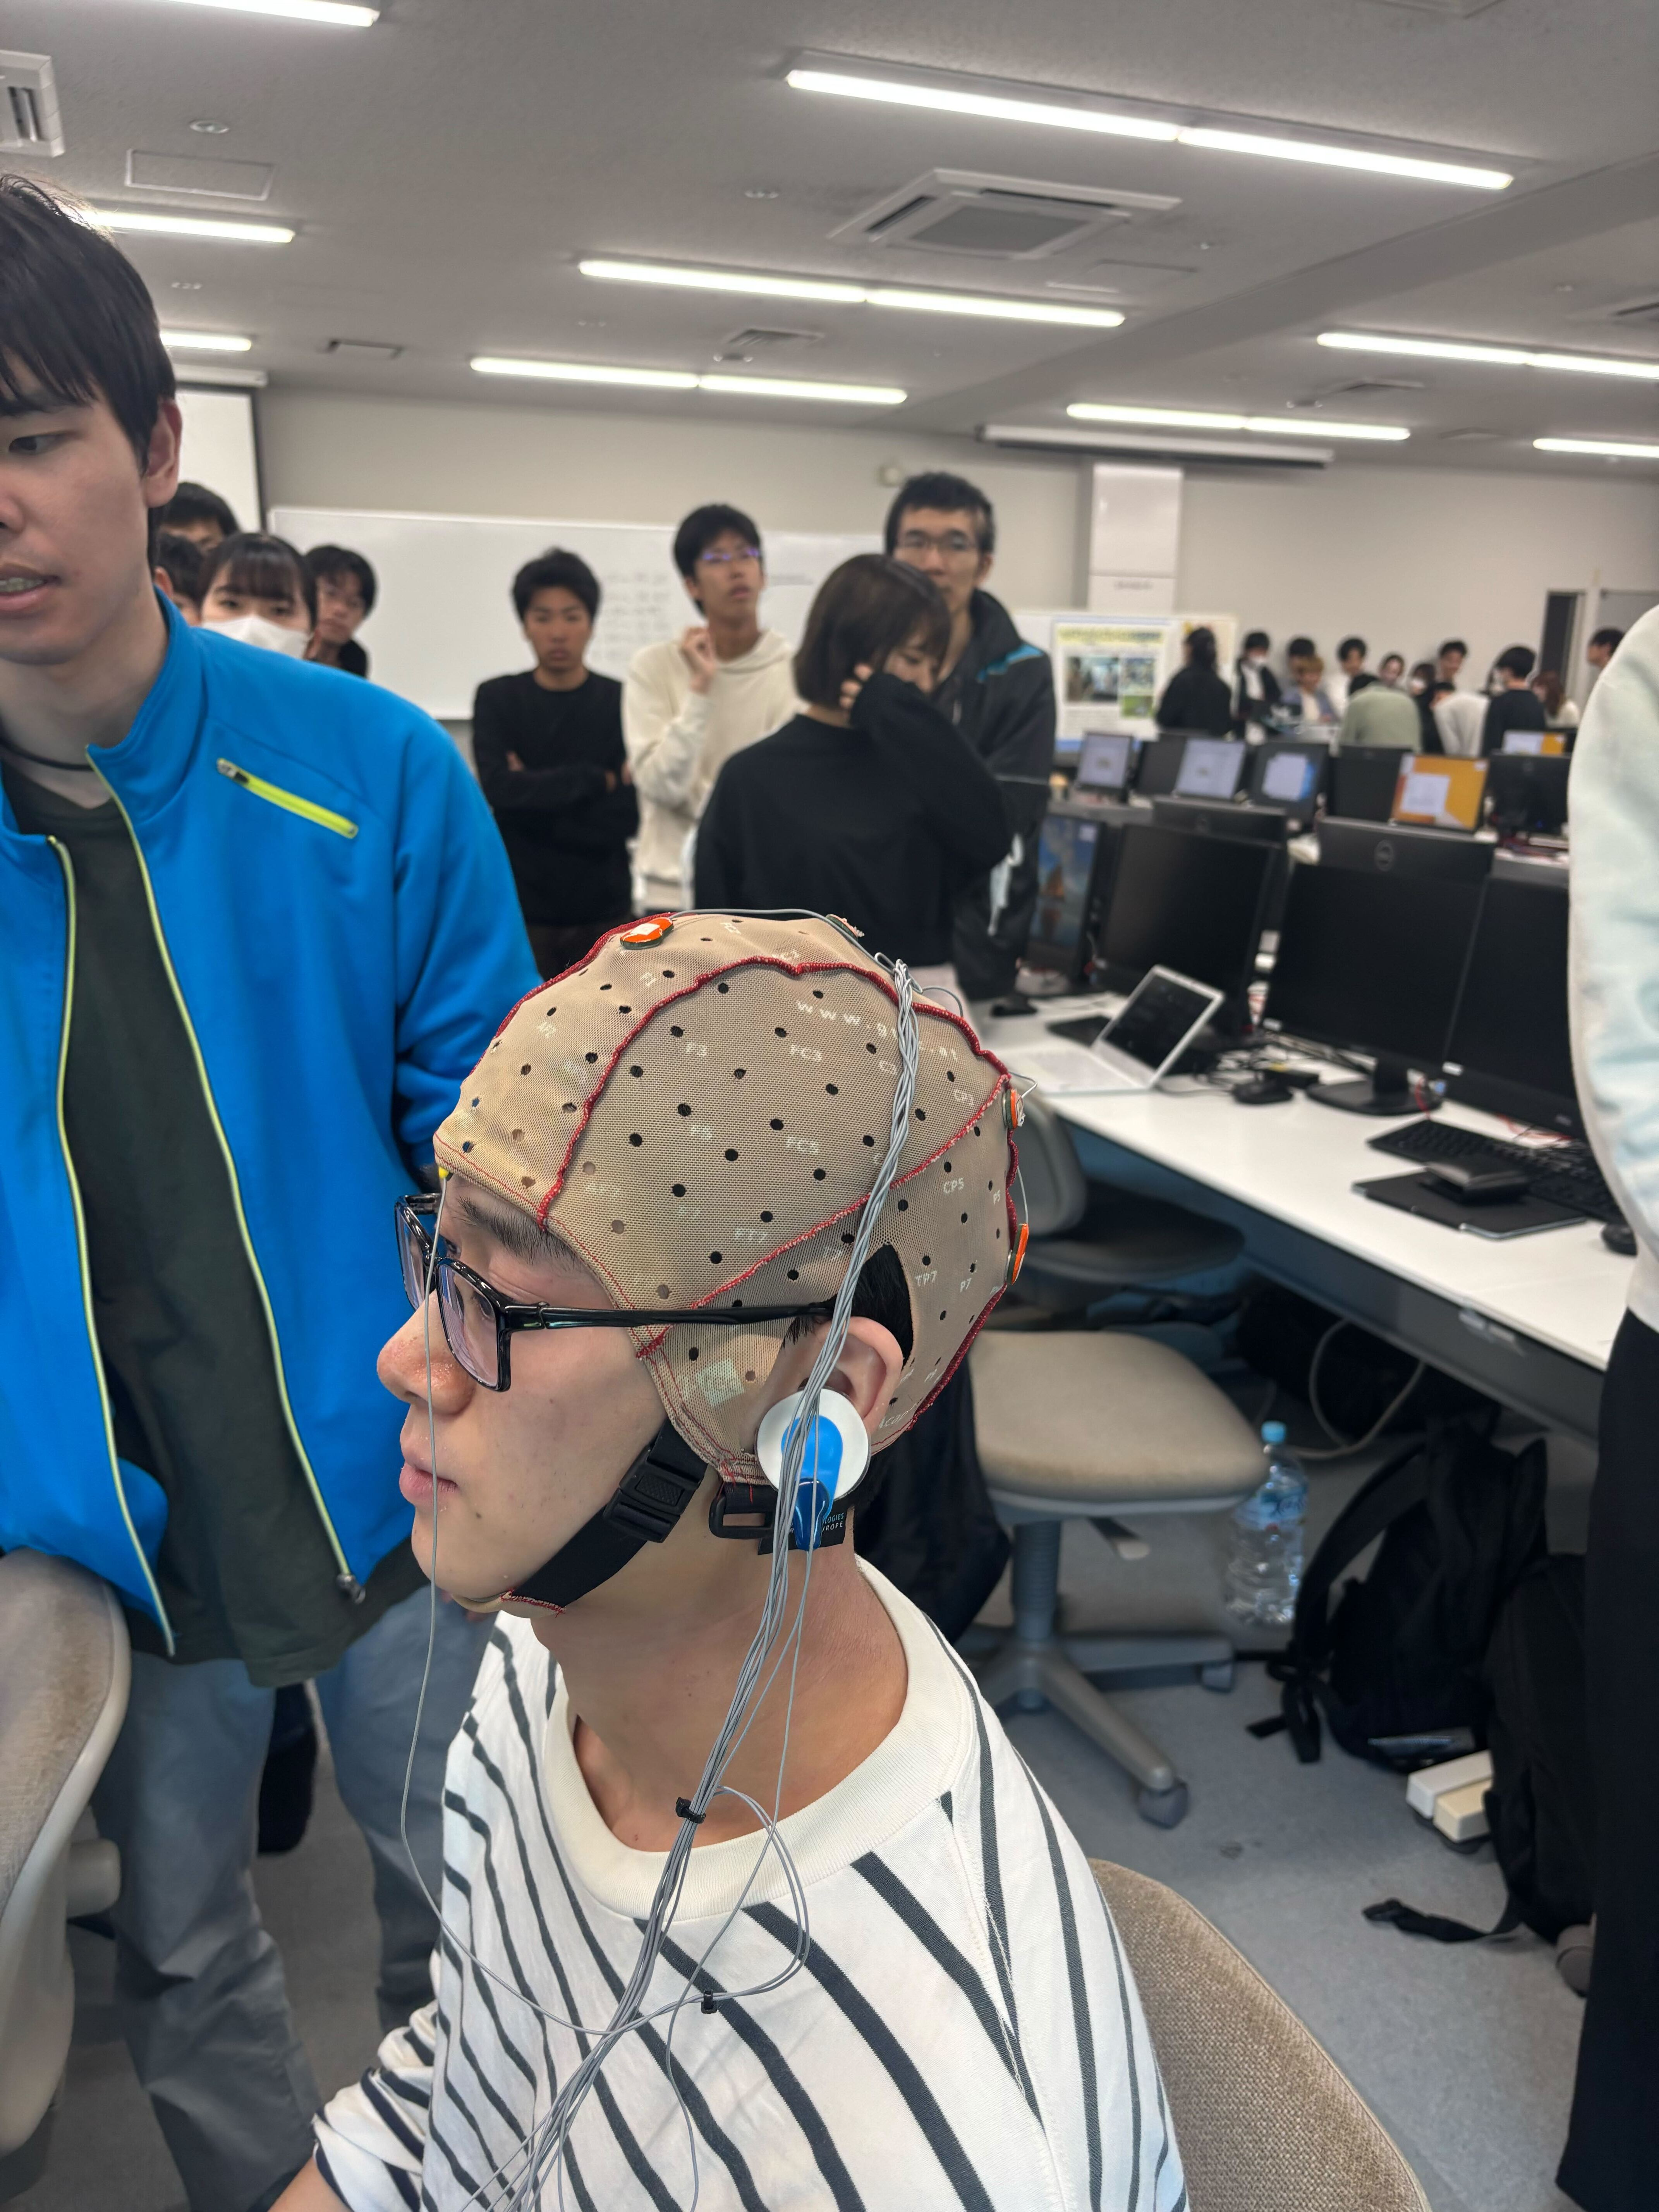
\includegraphics[keepaspectratio, width=0.6\linewidth]{figure/keisoku.jpg}
        \caption{脳波計測の実験風景}
        \label{fig:keisoku}
    \end{figure}


    \subsubsection{筋電計測}
    最大随意収縮及びダンベルを持っている時の上腕二頭筋の筋活動を計測する.まずは,LabChartを立ち上げる.今回は上腕二頭筋から筋活動を計測する.設置電極は肩峰とする.電極間の距離は約 2cm とする.サンプリング周波数は 1000Hz とする.

    最大随意収縮の計測については,安静状態から腕を 90 度曲げた状態で机等の動かないものに対して等尺性収縮で最大筋力を発揮する.ダンベルについては,1kg, 3kg, 5kg を用いて安静状態から選んだダンベルを 90 度曲げた状態で保持中の筋活動を計測する. 実際の実験画像は 画像\ref{fig:musle}である


\begin{figure}[H] % [htbp] は図の配置の優先順位(here, top, bottom, page)
    \centering % 図全体を中央に配置する

    % 1つ目の図
    \begin{minipage}[b]{0.32\linewidth}
        \centering
        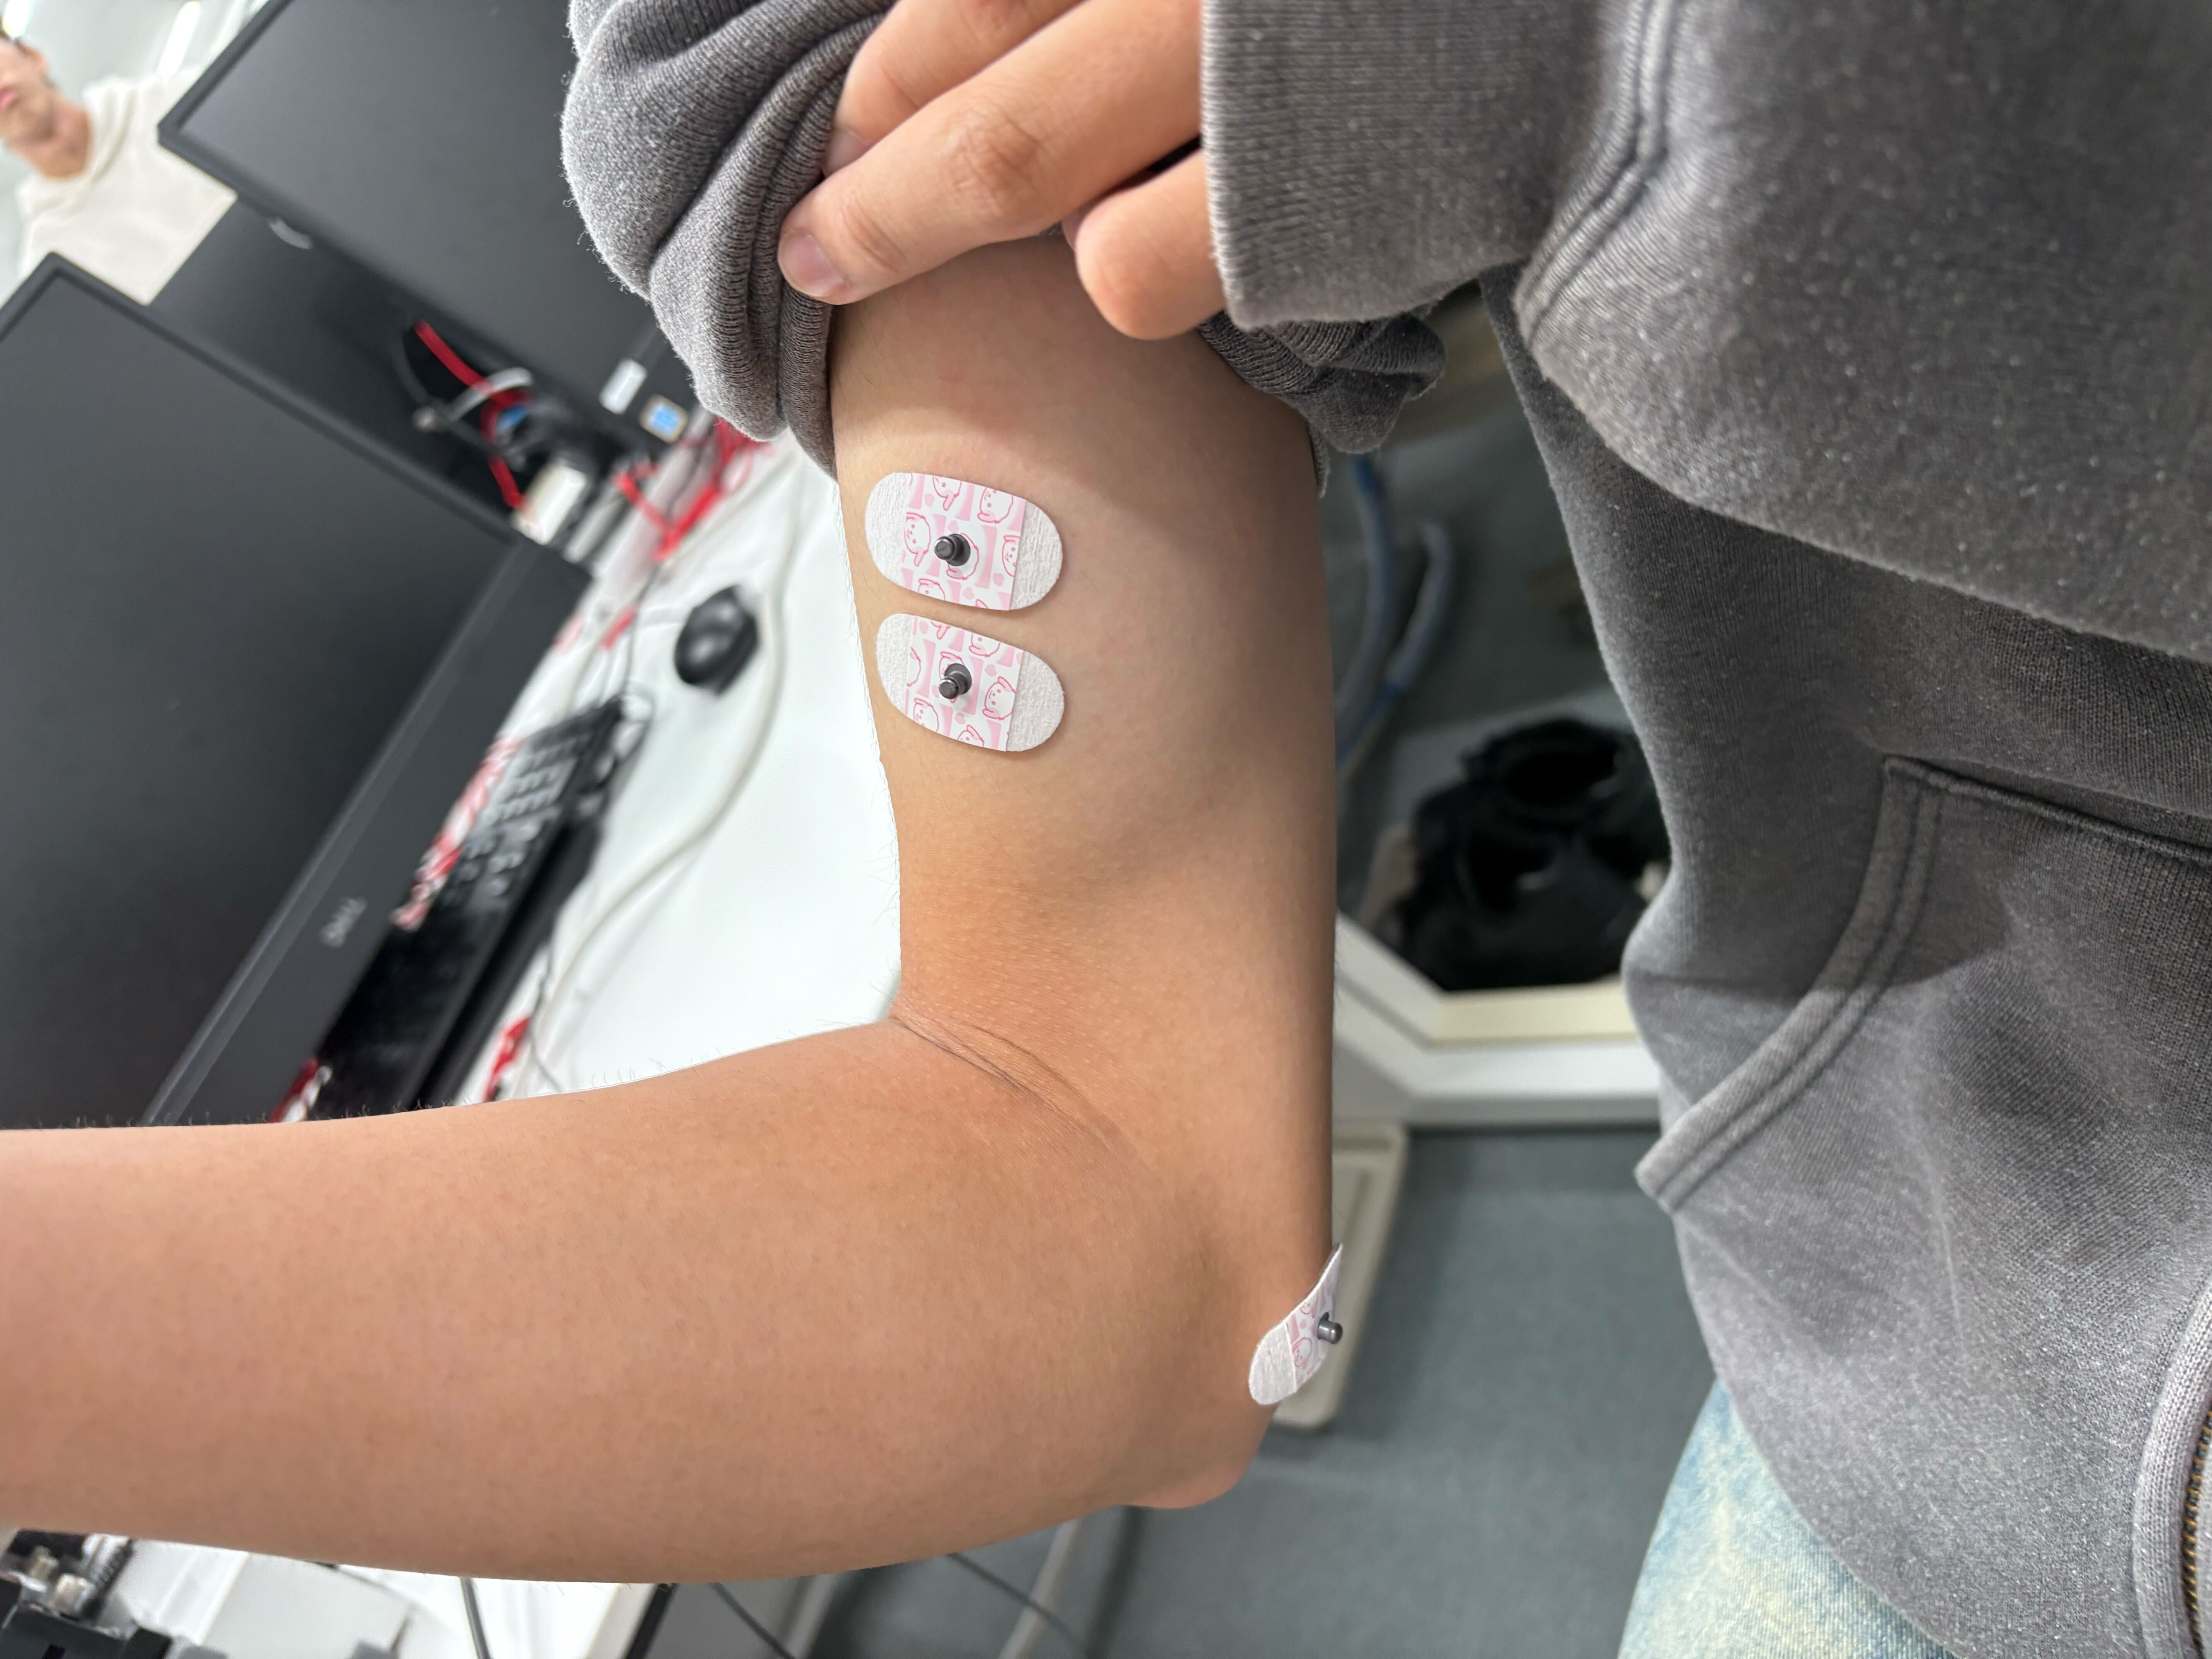
\includegraphics[width=\linewidth]{figure/IMG_6939.jpg} % 実際の画像ファイルパスに置き換える
    \end{minipage}
    \hfil
    % 2つ目の図
    \begin{minipage}[b]{0.32\linewidth}
        \centering
        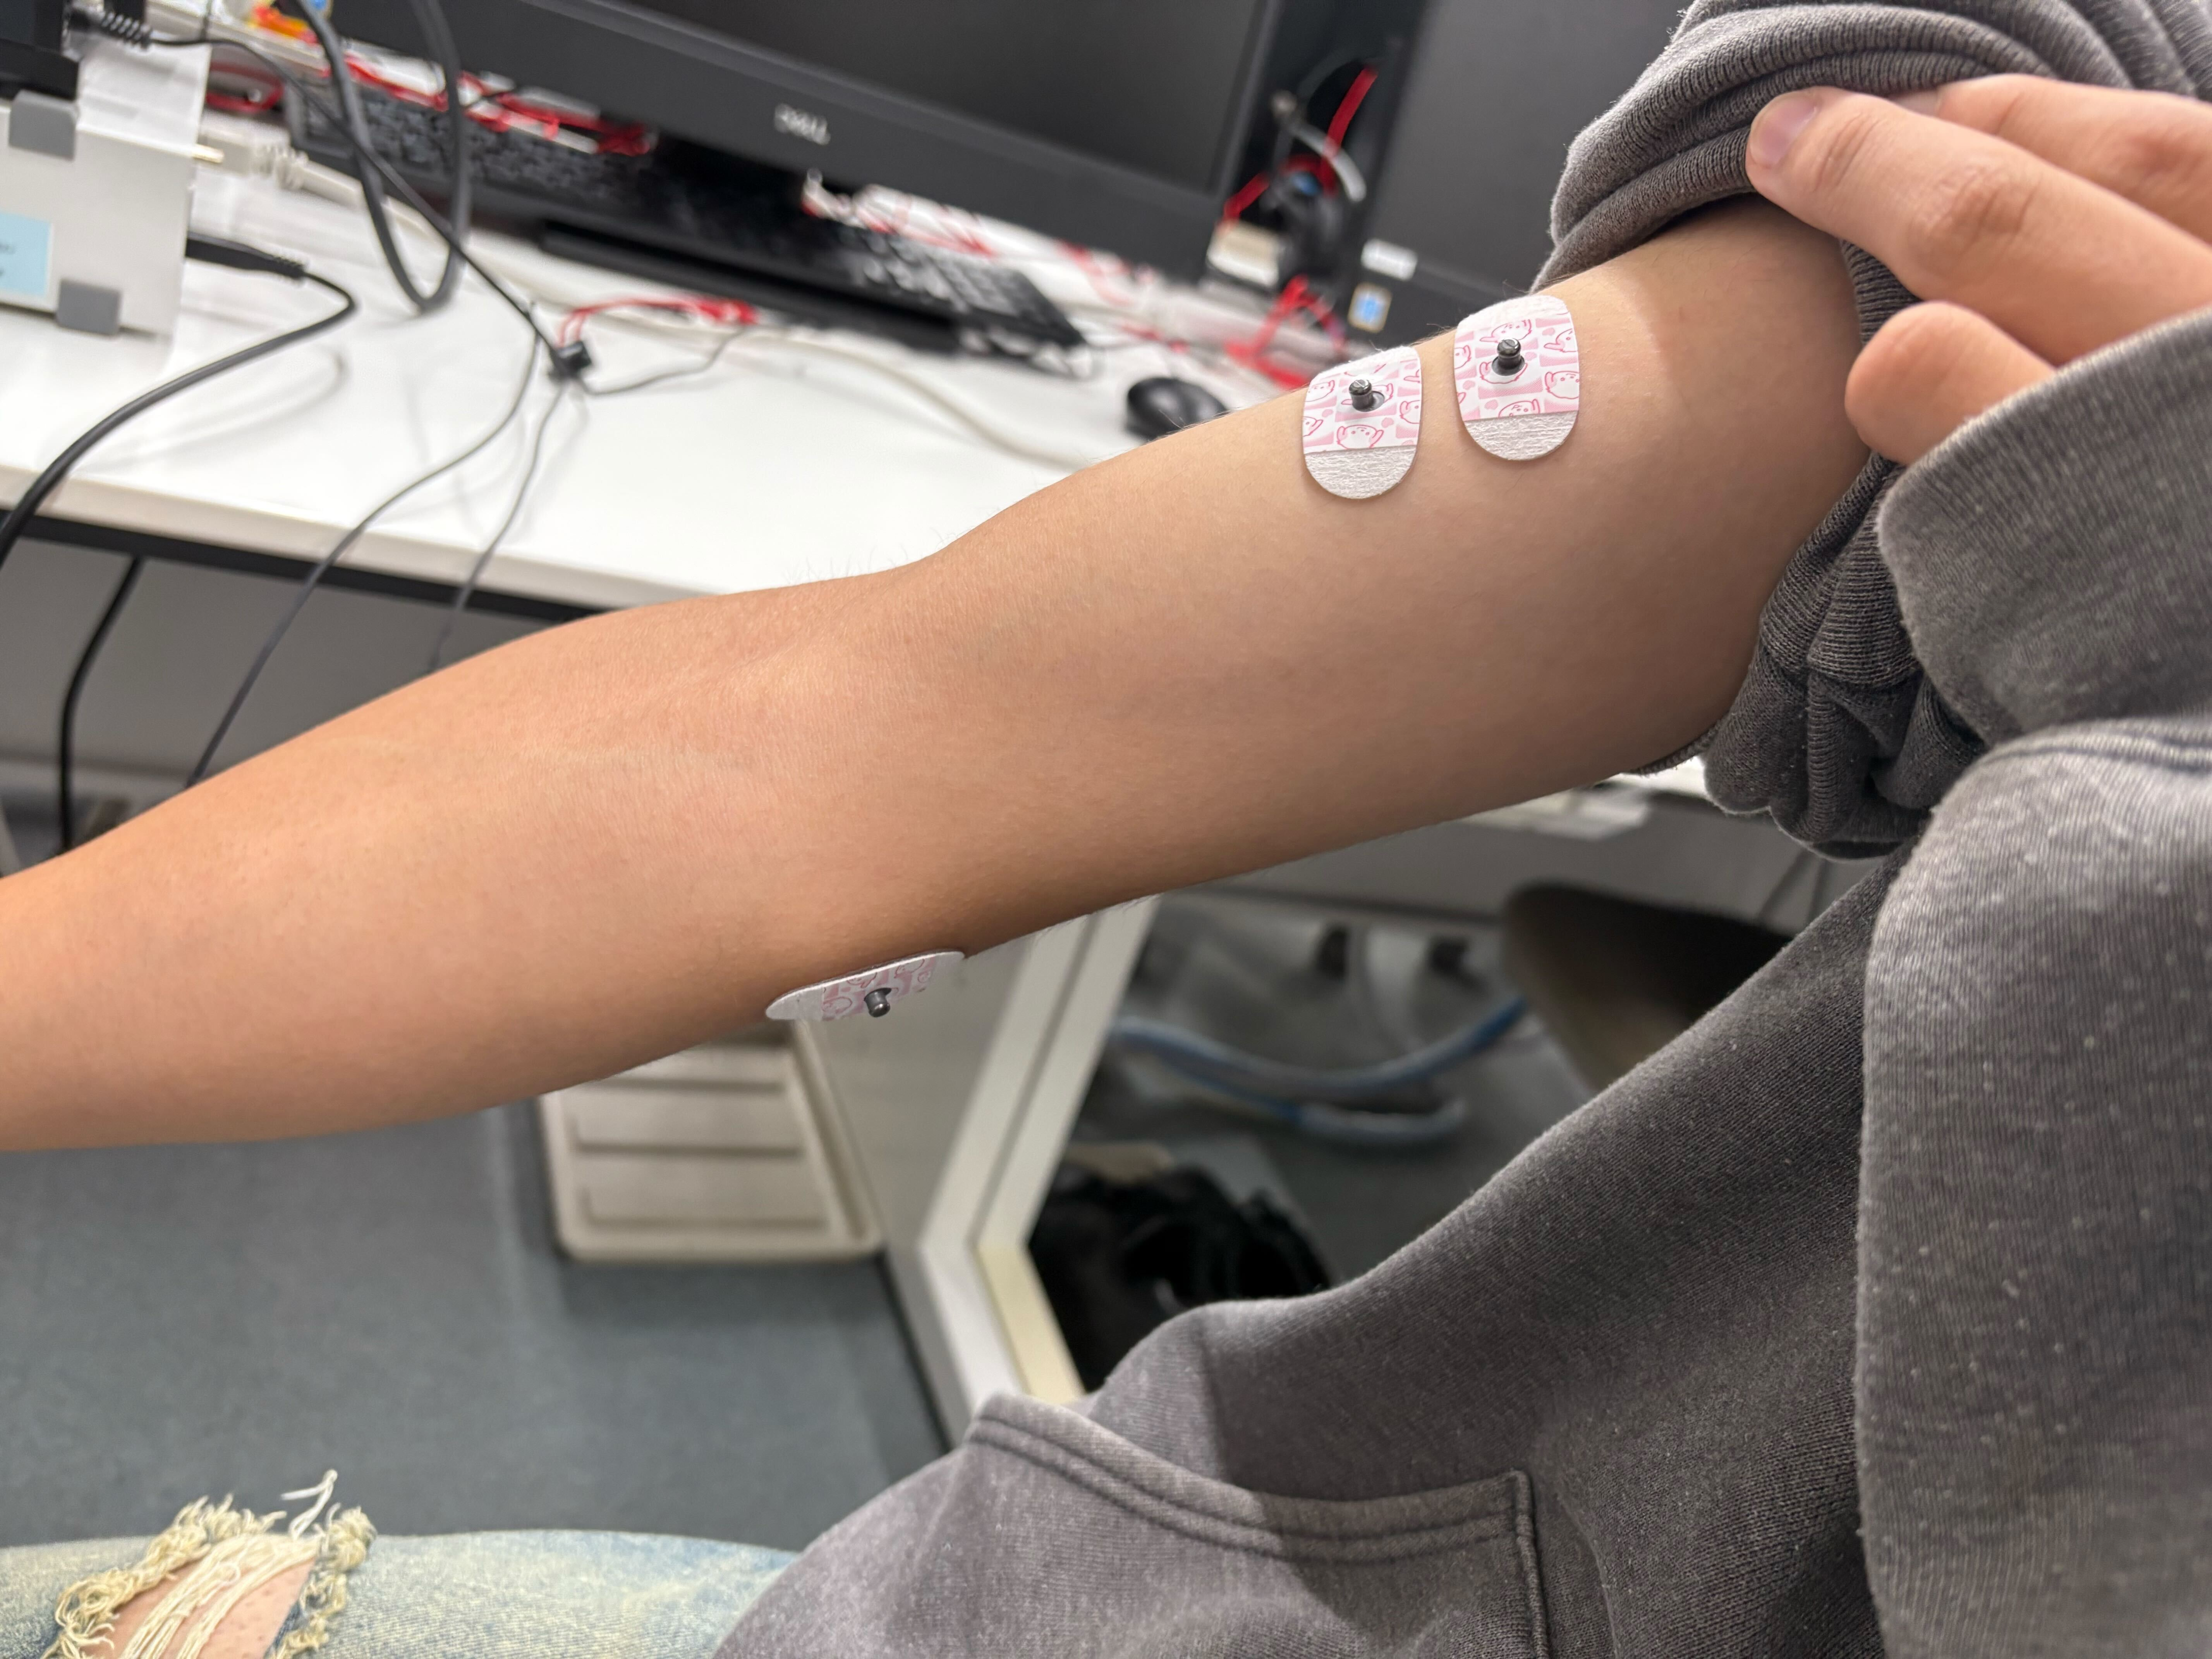
\includegraphics[width=\linewidth]{figure/IMG_6941.jpg} % 実際の画像ファイルパスに置き換える
    \end{minipage}
    \hfil
    % 3つ目の図
    \begin{minipage}[b]{0.32\linewidth}
        \centering
        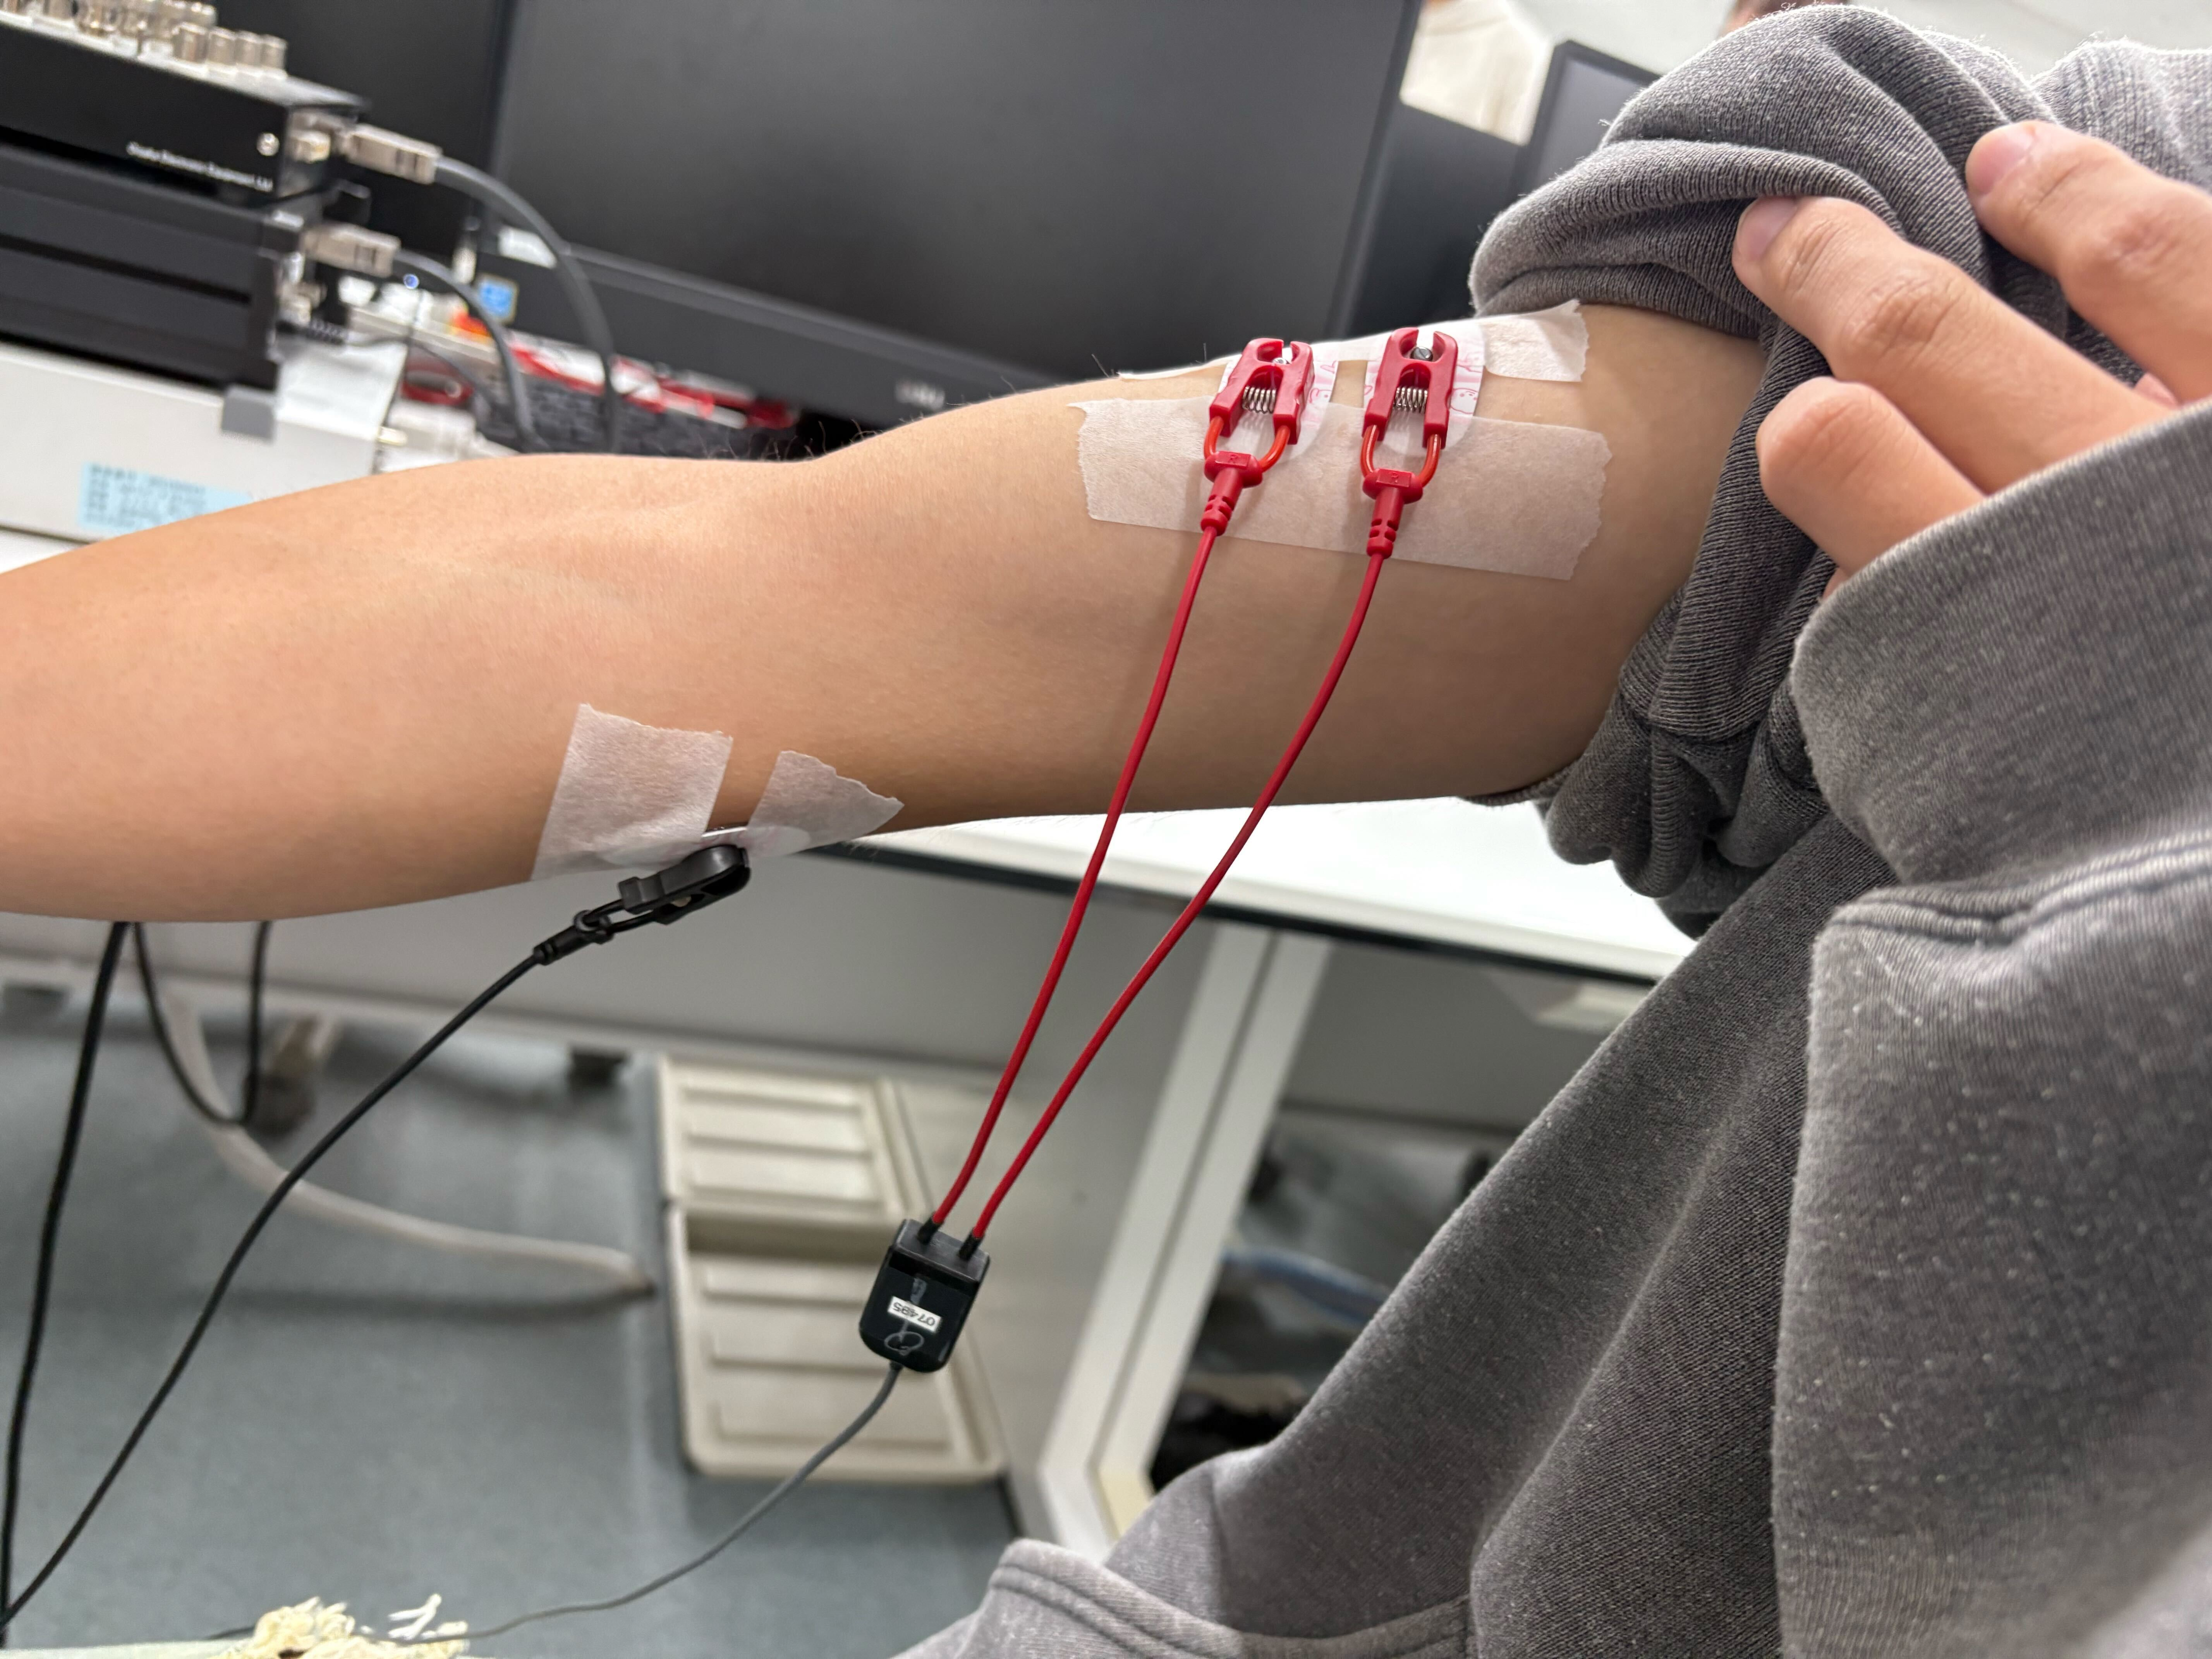
\includegraphics[width=\linewidth]{figure/IMG_6942.jpg} % 実際の画像ファイルパスに置き換える
    \end{minipage}
    \caption{筋電計測の実験風景} % 図全体に対するメインキャプションに置き換える
    \label{fig:musle} % 図全体に対する適切なラベルに置き換える
\end{figure}    

    \subsection{第九回の方法}
    結果を格納するための行列を作成する.行数はサンプリング周波数に対応する 500 行と列数は時間データ列と試行数となる.時間軸のデータについてはキー押しの 1 秒前からのデータを用いる.キーを押した時を 0msec として -998 までの 2msec おきの配列を作成する.これらを実装したコードがコード\ref{lst:exp3_9_vec}である.
    
    \begin{program}[H]
        \caption{結果格納用の準備}
        \inputminted[linenos,
        firstline=1,
        lastline=11,
        frame=lines,
        fontsize = \small]{matlab}{code/Exp3_9_Matlab.m}
        \label{lst:exp3_9_vec}
    \end{program}

    ここから各試行ごとにデータ処理を行っていく.キー押しの瞬間を基準とした相対的な時間軸を用いるため,キーを押した時刻を 0 の基準として,元々格納している時間である絶対時間を用いて相対時間を求める.それが以下のコード\ref{lst:exp3_9_expos}である.
    \begin{program}[H]
        \caption{注視データの整形}
        \inputminted[linenos,
        firstline=18,
        lastline=27,
        frame=lines,
        fontsize = \small]{matlab}{code/Exp3_9_Matlab.m}
        \label{lst:exp3_9_expos}
    \end{program}

    ここで,欠損値についても考えていく.欠損値とは,眼球運動の測定データにおいて,特定の時点でデータが取得されなかった場合や解析するにあたって無効なデータの場合は欠損として扱われる. EyeLink の測定では,まばたきやセンサの誤作動によってデータが欠けることがあるため, MatLab 上では欠損値として扱う.欠損データは -1 で初期化する.また,有効な行のみを対象に画面状態や X 座標を代入する.有効な行の識別は \mintinline{matlab}|ismember(expos(:, 1), eye_data(:, 1) - eye_data(end, 1))| でき, expos の各時間点で実際の眼球データが存在するかを確認する.
    その結果から有効な行のインデックスを取得する.expos の各列は以下の形式で入力を行う.
    \begin{enumerate}[label=\arabic*列目]
        \item 時間
        \item 測定する目の情報
        \item 両目の状態
        \item 左目注視位置 X座標
        \item 左目注視位置 Y座標
        \item 左目瞳孔径
    \end{enumerate}
    この列に対応した情報を入れていくが有効な行のみを対象とするため, ismember で取得したインデックスを用いて行う.これらのコードをコード\ref{lst:exp3_9_missing}に示す.

    \begin{program}[H]
        \caption{欠損値の処理}
        \inputminted[linenos,
        firstline=29,
        lastline=48,
        frame=lines,
        fontsize = \small]{matlab}{code/Exp3_9_Matlab.m}
        \label{lst:exp3_9_missing}
    \end{program}

    これから,注視位置の判定を行う.画像提示時のうち,x 座標を取得し,これらの平均値を計算する.この平均値の四捨五入したものがその試行における画面の中心 x 座標とする.この中心よりも左であるならば左側の画像を選択したと判断し,右であれば右側の画像を選択したと判断する.ここで,左側を見ていた場合を 100, 右側を見ていたなら 102 とする.画像提示時は expos の 3 列目に格納されており,その時の値は 2 であれば刺激画像を提示してる時である.また,左目の注視位置は, 5 列目に格納されており,中心よりも左であるか右であるかの論理積を取ることでそれぞれ求めることができる.これらのコードをコード\ref{lst:exp3_9_select}に示す.
    \begin{program}[H]
        \caption{注視位置の判定}
        \inputminted[linenos,
        firstline=50,
        lastline=58,
        frame=lines,
        fontsize = \small]{matlab}{code/Exp3_9_Matlab.m}
        \label{lst:exp3_9_select}
    \end{program}

    注視方向と選択の位置判定はキー押しの選択と視線が一致していたら 1, 一致していなければ 0 とする.これを行うために expos の 3 列目の値が 2 の時に選択位置と注視位置の判定を行う.また,選択位置は 100, 102 のどちらかであり,注視位置は -1, 1 のどちらかであるため,それらの論理積を取ることで一致しているかを判定する. どちらの顔画像が魅力的かを判断したデータは data という行列の 2 行目に格納されているため,そのデータとキーコードが一致しているかを確認する.また,キー押し直線の一秒間に限定して,被験者が最終的に魅力的だと判断した画像を見ていたかどうかをのデータを格納する.
    これらを実装したコードをコード\ref{lst:exp3_9_match}に示す.
    \begin{program}[H]
        \caption{注視位置と選択位置の一致}
        \inputminted[linenos,
        firstline=60,
        lastline=76,
        frame=lines,
        fontsize = \small]{matlab}{code/Exp3_9_Matlab.m}
        \label{lst:exp3_9_match}
    \end{program}
    コード\ref{lst:exp3_9_match_rate}では,全試行のデータが格納されている \mintinline{matlab}|data_matrix| をもとに,キー押し前の各時点において,平均してどのくらいの割合で被験者が最終的に選択した魅力的な画像をを見ていたのかを求める.500 行 1 列のゼロベクトルを用意する.その後,そのベクトルに抽出されたデータの平均値を計算する.0 と 1 のデータセットの平均値は,1 の割合を表す.したがって,\mintinline{matlab}|mean_valid_data| には, j の場合において有効な試行データの中で魅力的な画像を見ていた試行の割合が格納される.
    \begin{program}[H]
        \caption{注視位置と選択位置の一致率}
        \inputminted[linenos,
        firstline=79,
        lastline=91,
        frame=lines,
        fontsize = \small]{matlab}{code/Exp3_9_Matlab.m}
        \label{lst:exp3_9_match_rate}
    \end{program}

    全試行分の統計として,各時間ごとに視線が魅力的な画像と一致していた割合を計算する.結果を時間軸に沿ってグラフ描画する.これをコード\ref{lst:exp3_9_plot}に示す.
    \begin{program}[H]
        \caption{注視位置と選択位置の一致率のグラフ化}
        \inputminted[linenos,
        firstline=92,
        lastline=96,
        frame=lines,
        fontsize = \small]{matlab}{code/Exp3_9_Matlab.m}
        \label{lst:exp3_9_plot}
    \end{program}

    \subsection{第十回の方法}
    まず,読み込んだテキストファイルから筋電データを読み込む.次に,筋電データを plot 関数を用いて読み込んだ各条件のデータを描画し,視覚的に確認するコードをコード\ref{lst:3_10_plot}に示す.

    \begin{program}[H]
        \caption{筋電データの読み込みと描画}
        \inputminted[linenos,
        firstline=1,
        lastline=29,
        frame=lines,
        fontsize=\small]{matlab}{code/Exp3_10_Matlab.m}
        \label{lst:3_10_plot}
    \end{program}


    コード\ref{lst:3_10_plot} を実行した結果が図\ref{fig:all_four_images}である.

    \begin{figure}[H] % [htbp] は図の配置の優先順位
    \centering % 全体の図を中央揃えにする

    % --- 上段の2つの図 ---
    \begin{subfigure}[b]{0.48\linewidth} % ページの幅の約48%を各図に割り当てる
        \centering
        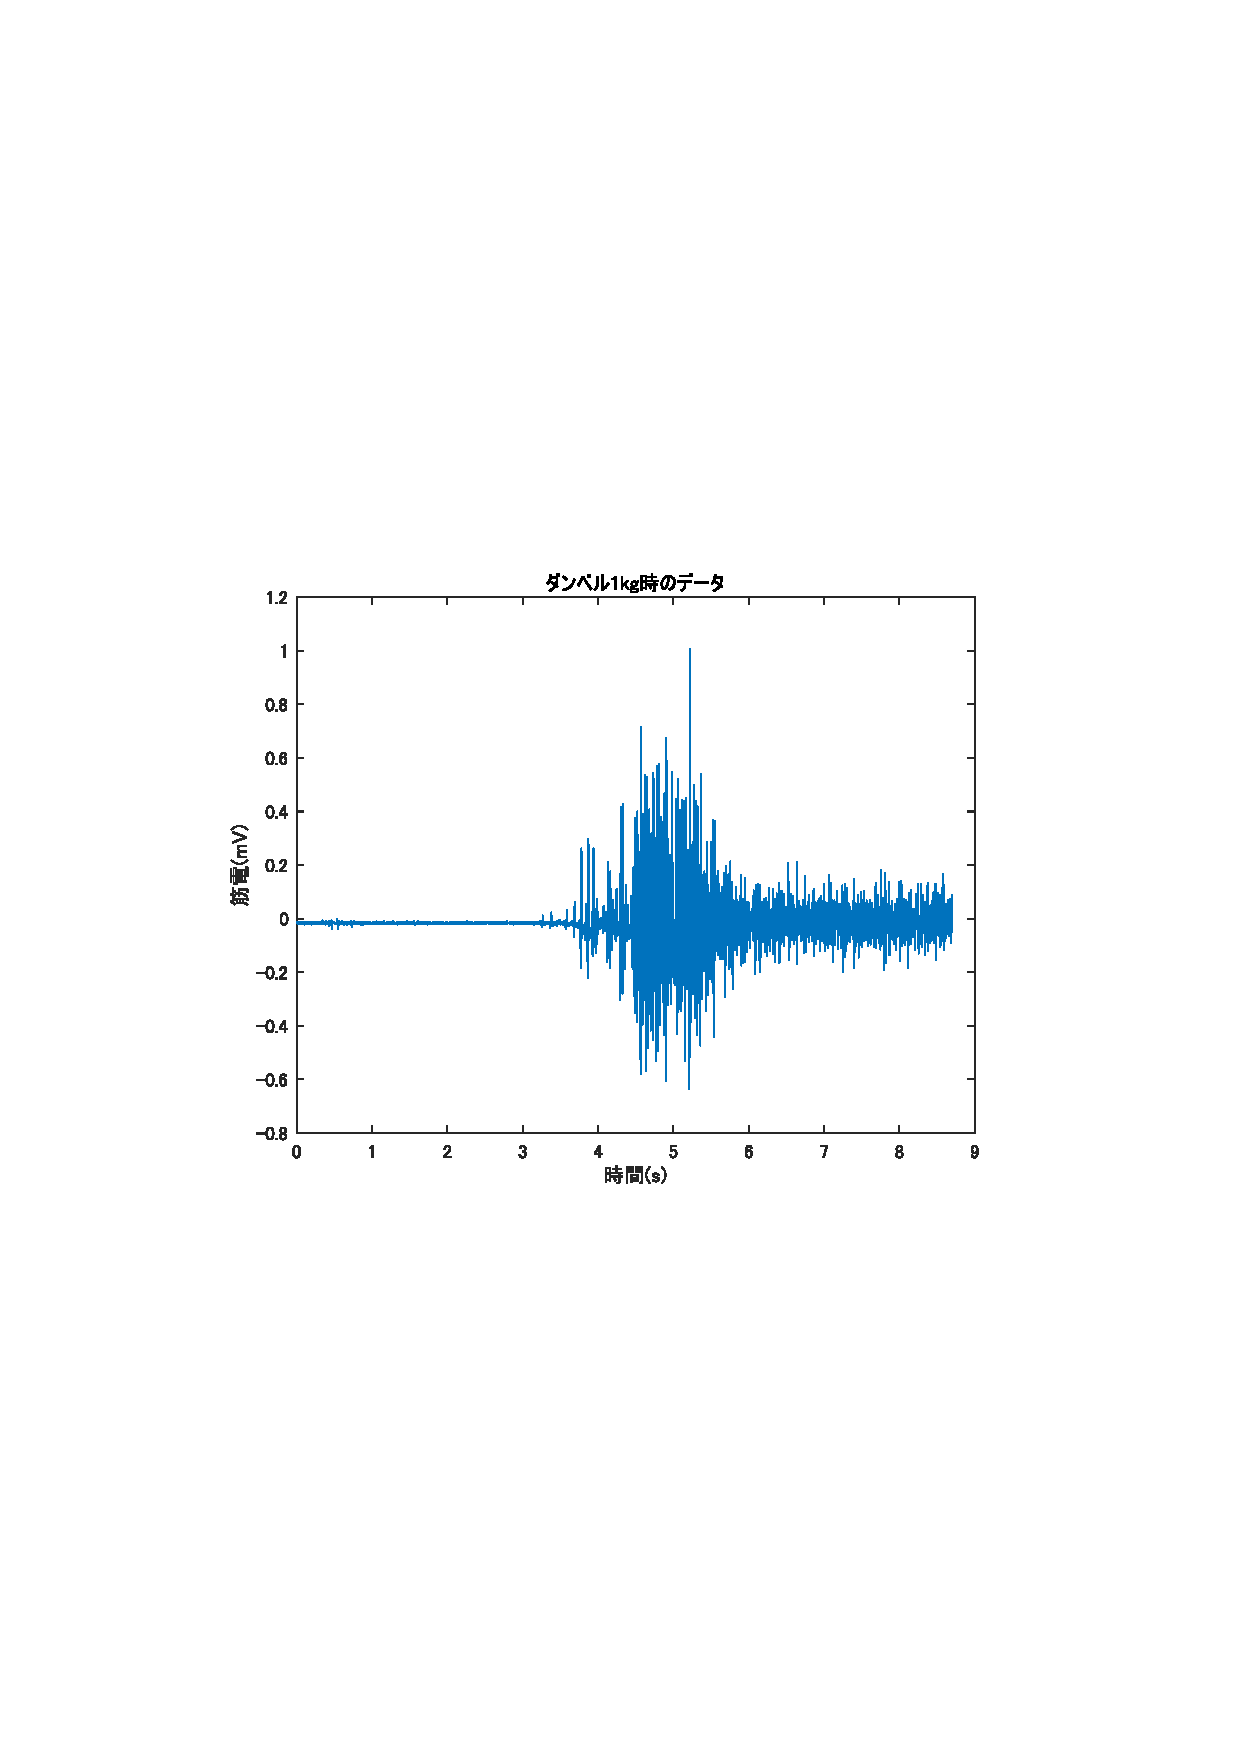
\includegraphics[trim=90 250 100 250 clip,width=\linewidth]{figure/data_1kg.pdf} % サブfigureの幅に合わせて画像を調整
        \caption{MVCの時のデータ} % (a) と表示される
        \label{fig:suba}
    \end{subfigure}
    \hfill % 残りの水平方向のスペースを均等に埋める
    \begin{subfigure}[b]{0.48\linewidth}
        \centering
        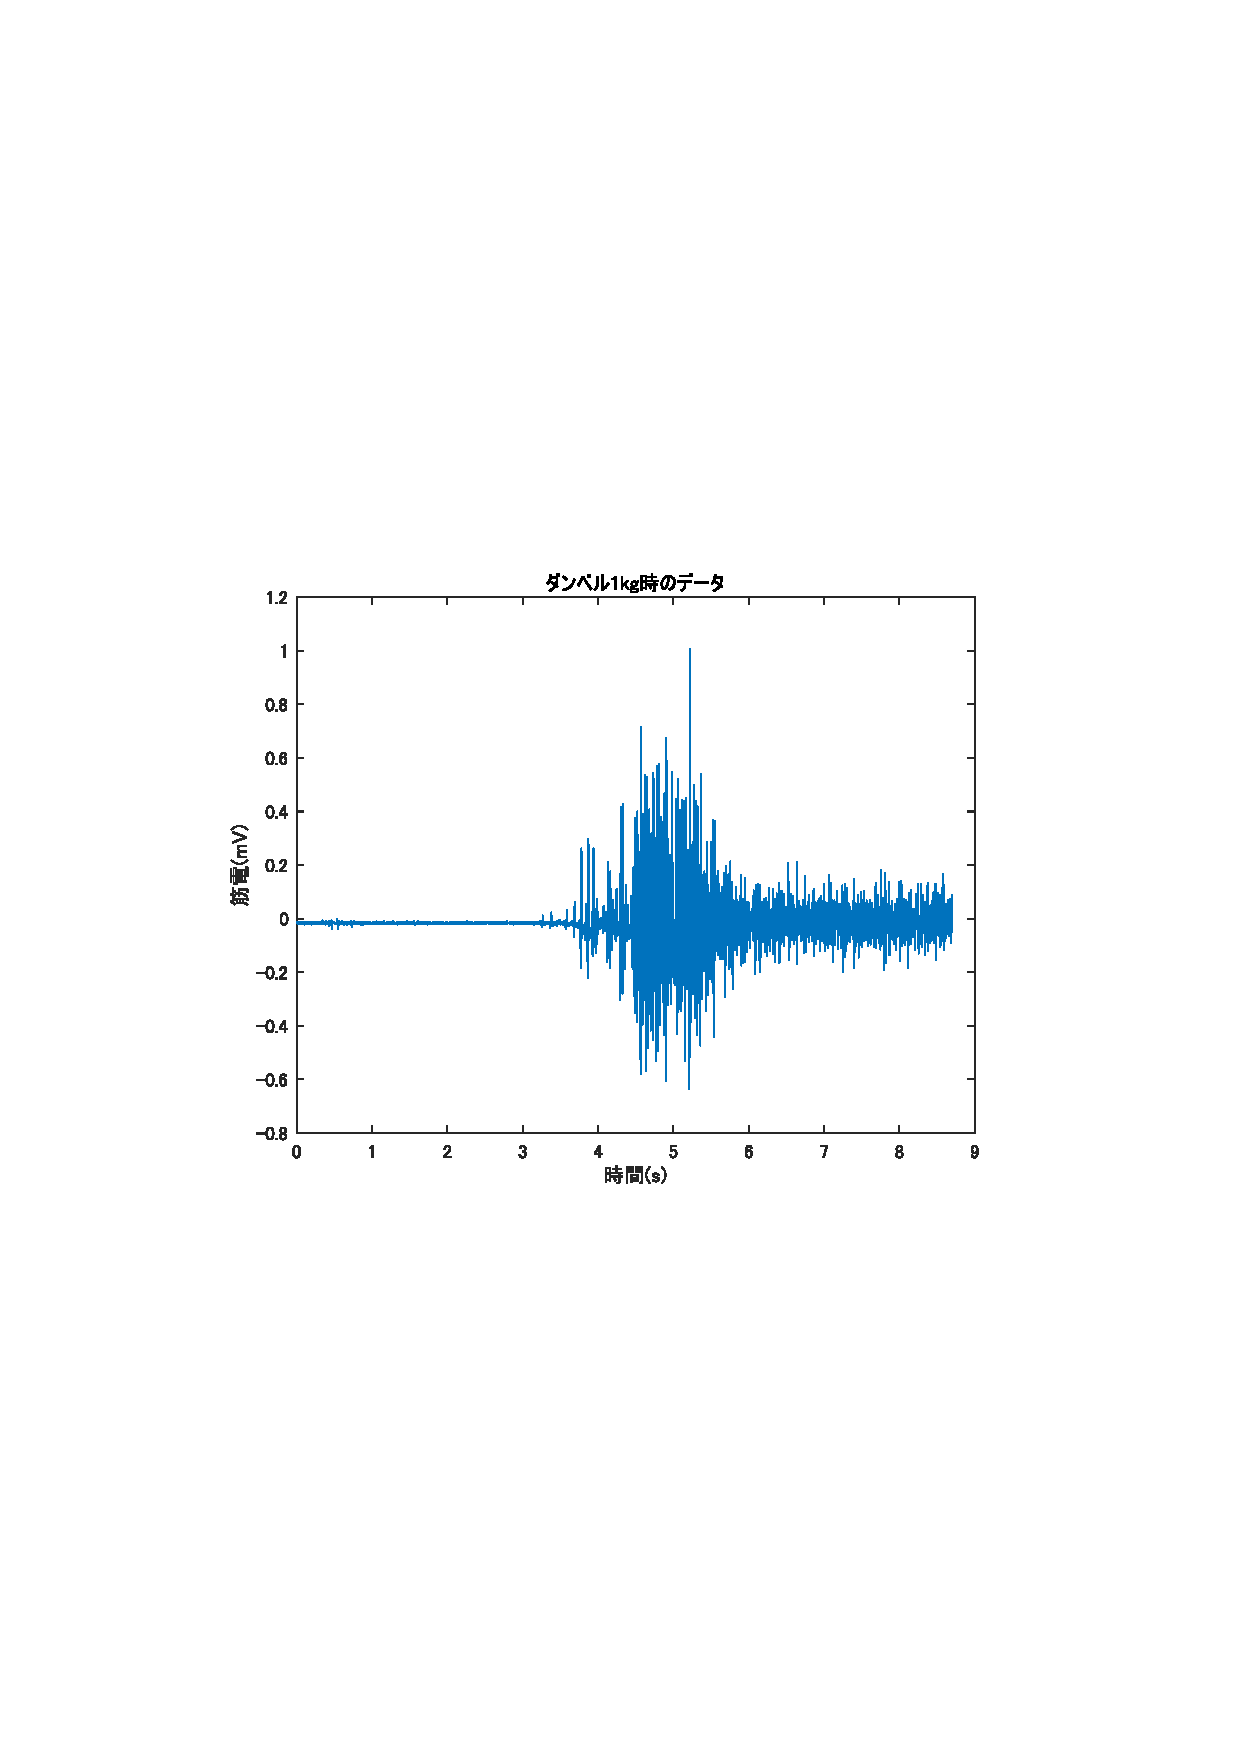
\includegraphics[trim=90 250 100 250 clip,width=\linewidth]{figure/data_1kg.pdf}
        \caption{ダンベルが1kgの時のデータ} % (b) と表示される
        \label{fig:subb}
    \end{subfigure}

    \vspace{1em} % 上段と下段の間に少し垂直方向のスペースを入れる (任意)

    % --- 下段の2つの図 ---
    \begin{subfigure}[b]{0.48\linewidth}
        \centering
        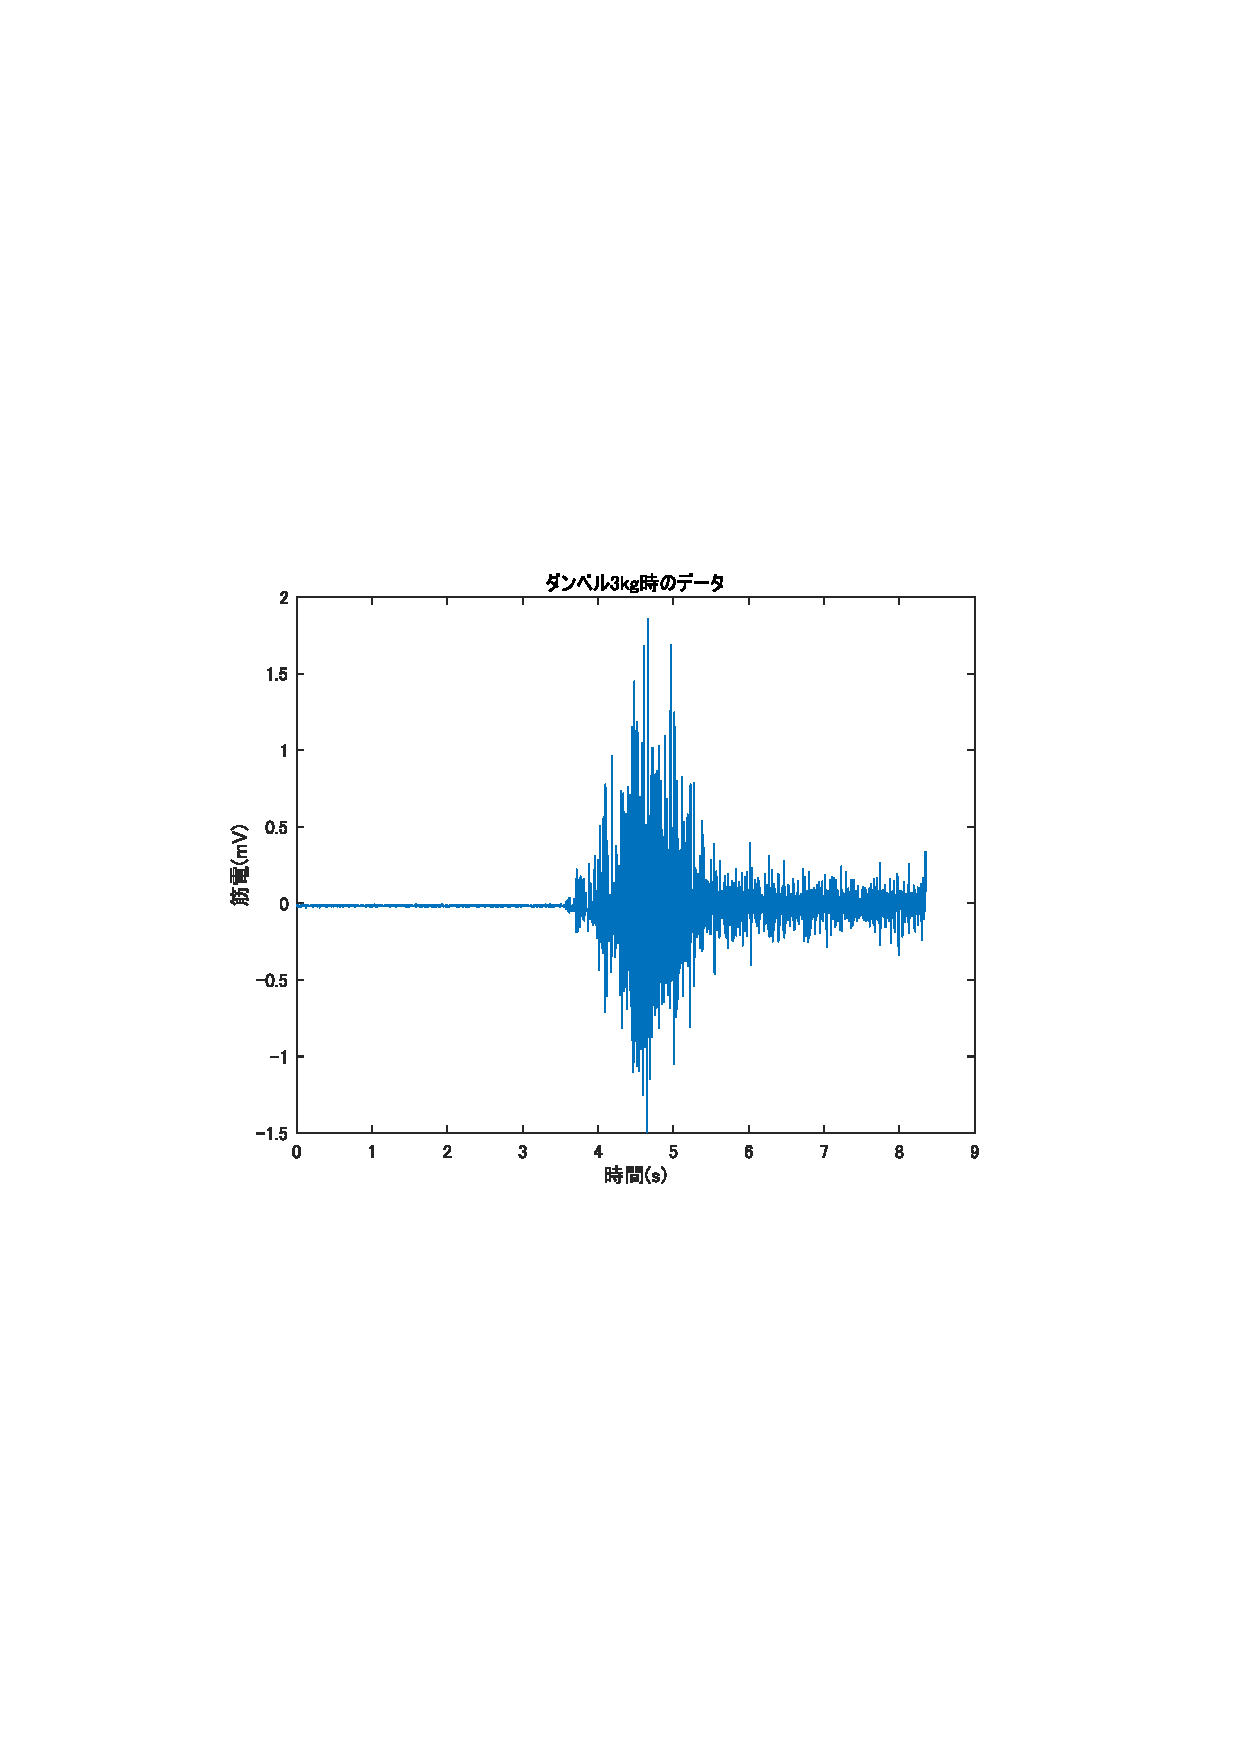
\includegraphics[trim=90 250 100 250 clip,width=\linewidth]{figure/data_3kg.pdf}
        \caption{ダンベルが3kgの時のデータ} % (c) と表示される
        \label{fig:subc}
    \end{subfigure}
    \hfill
    \begin{subfigure}[b]{0.48\linewidth}
        \centering
        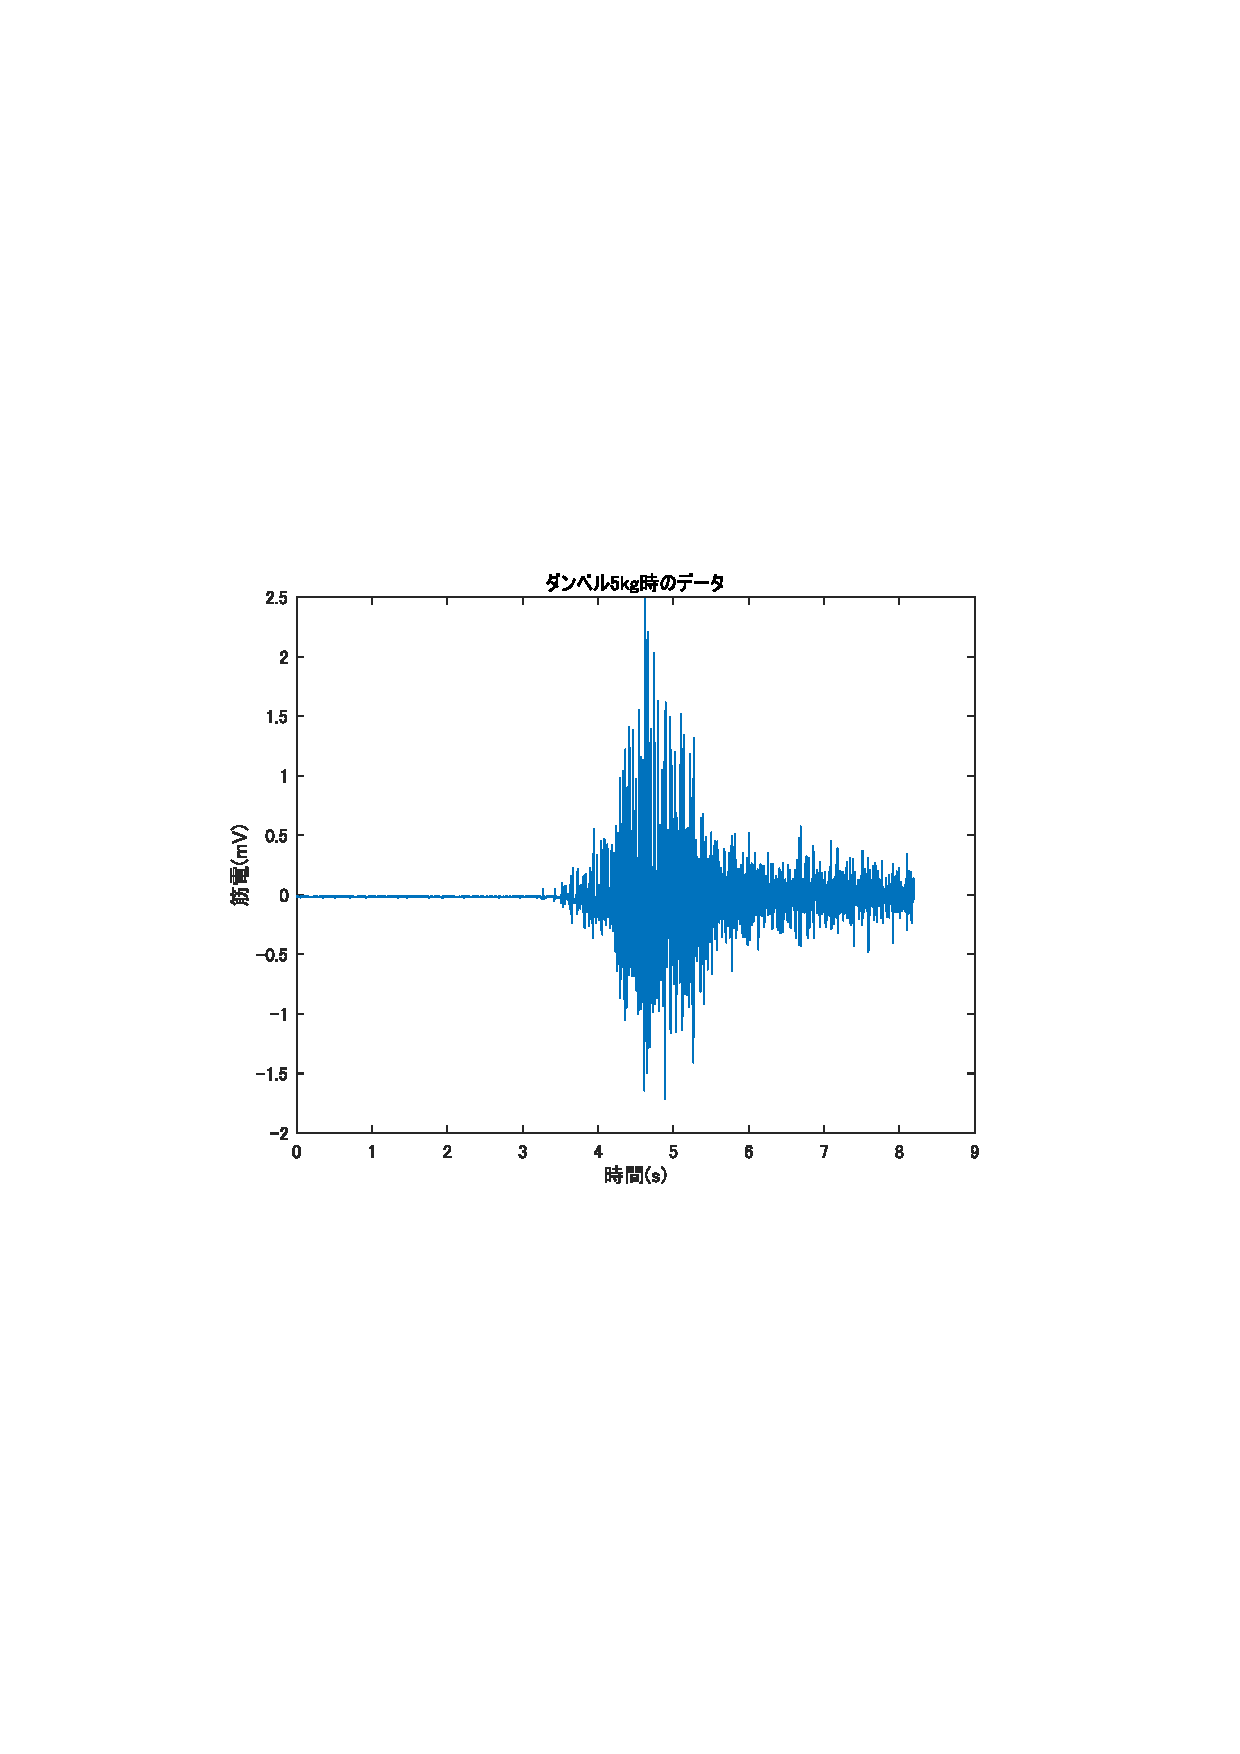
\includegraphics[trim=90 250 100 250 clip,width=\linewidth]{figure/data_5kg.pdf}
        \caption{ダンベルが5kgの時のデータ} % (d) と表示される
        \label{fig:subd}
    \end{subfigure}

    \caption{筋電計測で得られたデータ} % 図全体に対するキャプション
    \label{fig:all_four_images}
\end{figure}

    次に,最大随意収縮 (MVC) の解析を行う.MVC のデータは,dataBlocks{1} に格納されているため,このデータを用いる.コード\ref{lst:3_10_plot} で,表示したデータから筋活動が安定している安静時区間を目視で確認し,その区間の平均値をベースライン値として算出する.そこから,MVC の値を引くことで基線のずれを補正する.また,全波整流を行うためにベースライン補正後の MVC データを abs 関数を用いて絶対値化する.最後に,整流処理後のデータから max 関数を用いて最大値を取得する.
    \begin{program}[H]
        \caption{最大随意収縮 (MVC) の解析}
        \inputminted[linenos,
        firstline=31,
        lastline=50,
        frame=lines,
        fontsize = \small]{matlab}{code/Exp3_10_Matlab.m}
        \label{lst:3_10_mvc}
    \end{program}

    これから,MVC 以外の各負荷条件のデータに対して,処理を行なっていく.最初に,条件データの準備を行う.dataBlocks{2} から dataBlocks{5} までのデータをループを用いて抽出していき,抽出したデータの安静時区間をコード\ref{lst:3_10_plot} で出力されたグラフから出力されているため,目視で確認する.その区間の筋電位の平均値をベースラインとして算出後,データ全体から減算し,整流する.これらの実装をコード\ref{lst:3_10_load}に示す.

    \begin{program}[H]
        \caption{各負荷条件のデータの準備}
        \inputminted[linenos,
        firstline=53,
        lastline=73,
        frame=lines,
        fontsize = \small]{matlab}{code/Exp3_10_Matlab.m}
        \label{lst:3_10_load}
    \end{program}

    次に,電図データのノイズの除去,平滑化を目的してローパスフィルタ処理を設定する.サンプリング周波数を 1000Hz, カットオフ周波数 5Hz の2次バターワースローパスフィルタを butter 関数で設計する.この設定したファイルを filtfit 関数を用いて整流後のデータに適用し,平滑化を施す.filtfit 関数は位相の歪みを防ぐために順方向と逆方向からフィルタをかける.このフィルタ処理後のデータから,筋が安定して活動していると見なせる 1000ms 区間の平均値を求める.この筋が安定していると見なせる区間はコード\ref{lst:3_10_plot} で出力された図で確認できる.ここから特定した安定活動区間が適切であるかを確認するため,フィルタ処理後のデータと選択された区間の開始・
    終了位置をプロットする.ここで,分散が最も小さくなる区間をとする.これらの内容をコード\ref{lst:3_10_ana} に記す.

    \begin{program}[H]
        \caption{各負荷条件のデータの解析}
        \inputminted[linenos,
        firstline=76,
        lastline=113,
        frame=lines,
        fontsize = \small]{matlab}{code/Exp3_10_Matlab.m}
        \label{lst:3_10_ana}        
    \end{program}

    適切な区間が正しいかをグラフに出力して確かめ,正規化筋電を求め,結果を格納するベクトルに結果を入れる.これらの内容をコード\ref{lst:3_10_norm}に示す.

    \begin{program}[H]
        \caption{各負荷条件の正規化}
        \inputminted[linenos,
        firstline=118,
        lastline=140,
        frame=lines,
        fontsize = \small]{matlab}{code/Exp3_10_Matlab.m}
        \label{lst:3_10_norm}
    \end{program}

\begin{figure}[H] % [htbp] は図の配置の優先順位(here, top, bottom, page)
    \centering % 図を中央に配置する

    % 1つ目の図
    \begin{subfigure}[b]{0.32\linewidth} % ページの幅の約32%を各図に割り当てる (3つで96%程度)
        \centering
        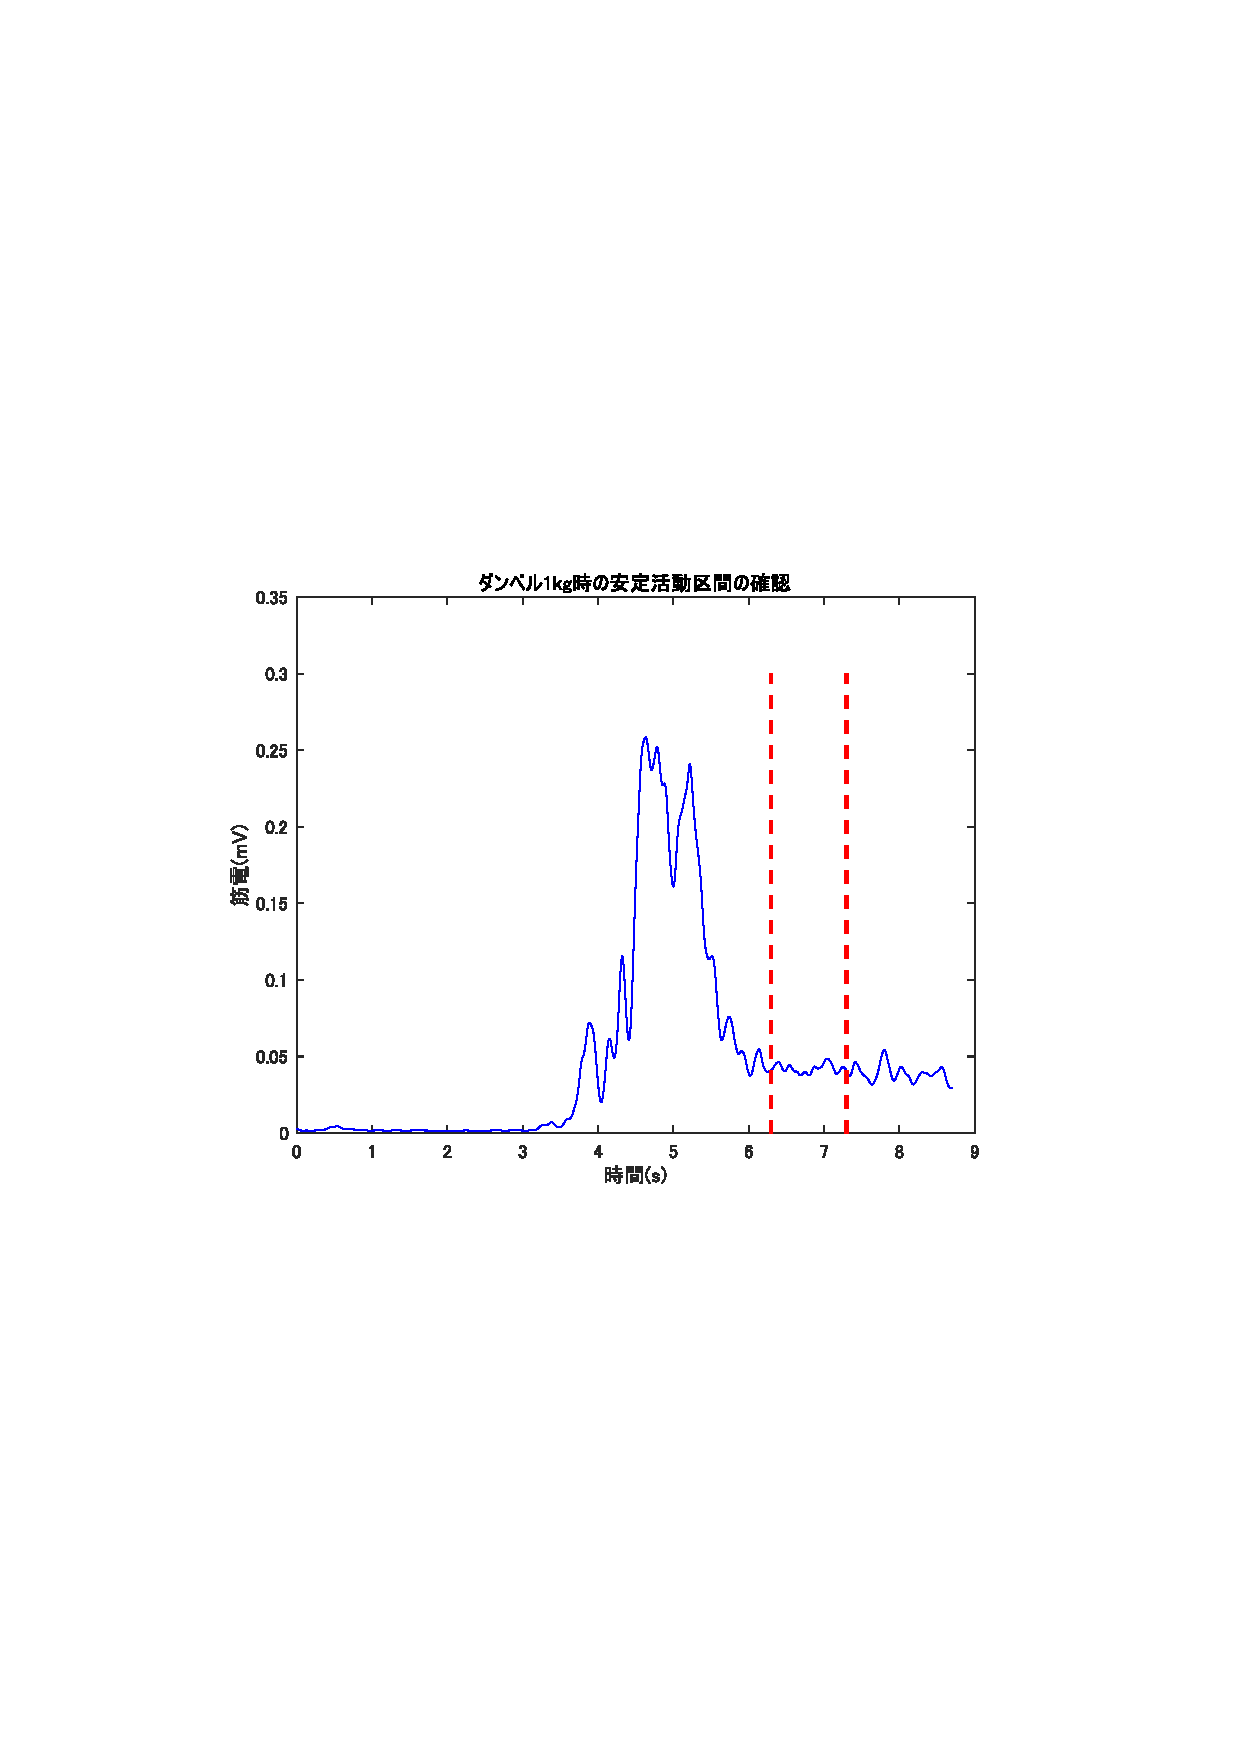
\includegraphics[trim=90 250 100 250 clip,width=\linewidth]{figure/check_1kg.pdf} % サブfigureの幅に合わせて画像を調整
        \caption{1kg 時のデータ} % 各図のサブキャプション
        \label{fig:cha}
    \end{subfigure}
    \hfill % 図と図の間にスペースを均等に配置する
    % 2つ目の図
    \begin{subfigure}[b]{0.32\linewidth}
        \centering
        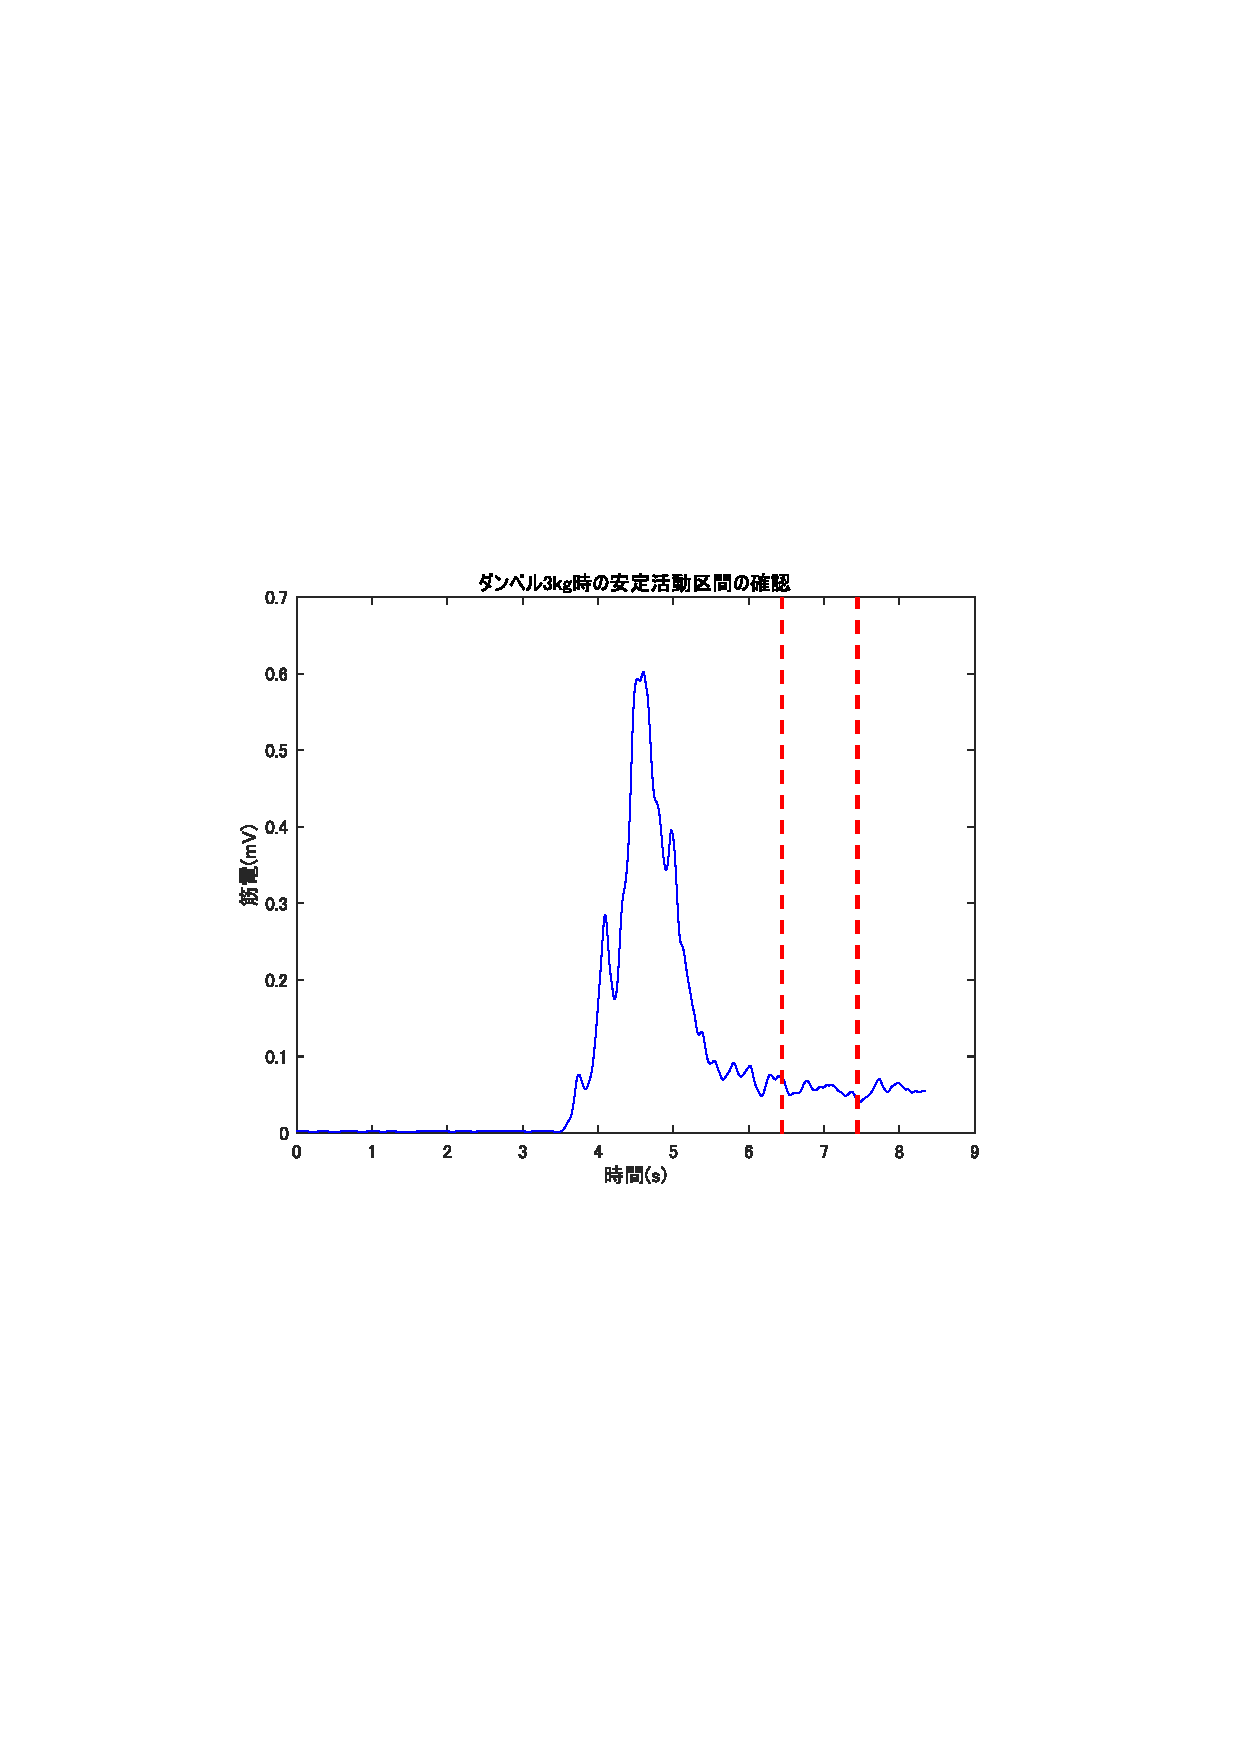
\includegraphics[trim=90 250 100 250 clip,width=\linewidth]{figure/check_3kg.pdf}
        \caption{3kg 時のデータ}
        \label{fig:chb}
    \end{subfigure}
    \hfill
    % 3つ目の図
    \begin{subfigure}[b]{0.32\linewidth}
        \centering
        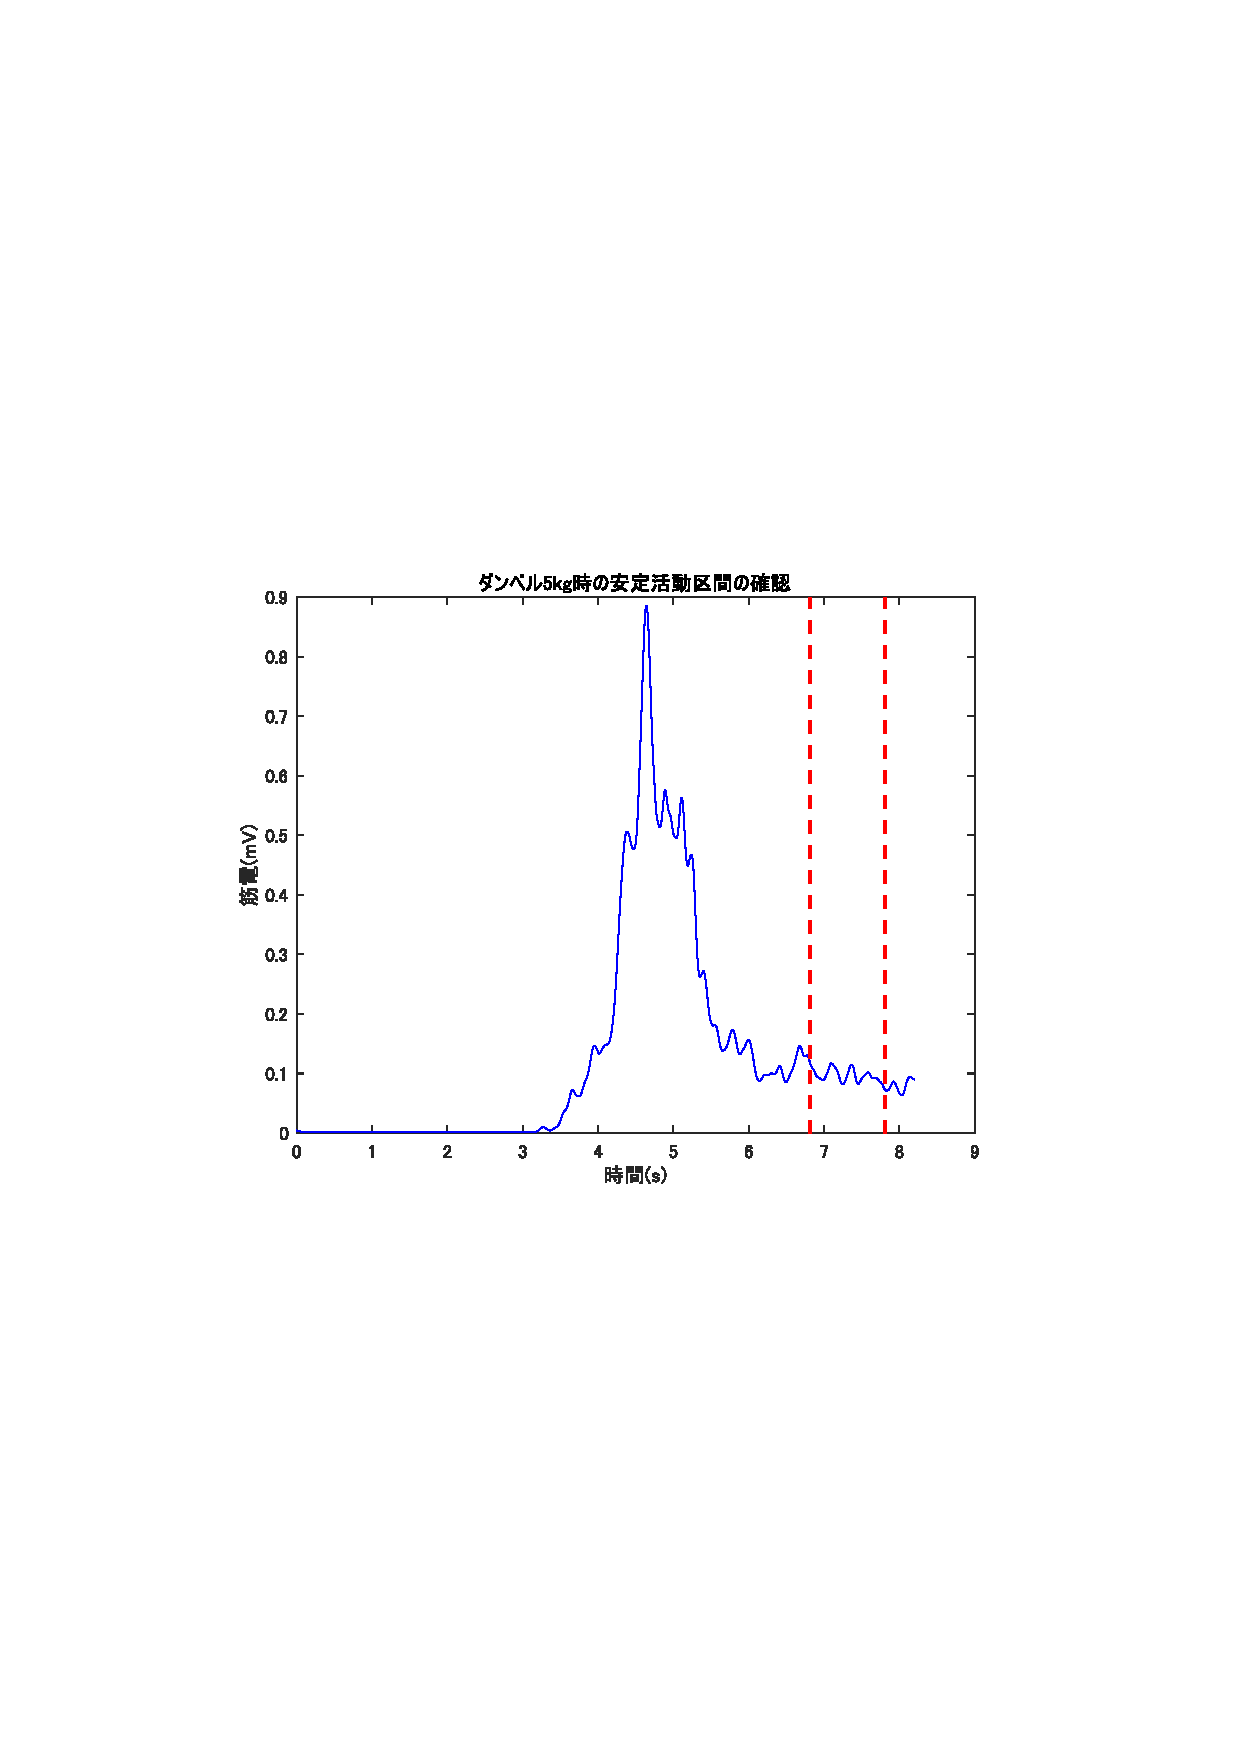
\includegraphics[trim=90 250 100 250 clip,width=\linewidth]{figure/check_5kg.pdf}
        \caption{5kg 時のデータ}
        \label{fig:chc}
    \end{subfigure}

    \caption{安静時区間が適切かを確かめるためのグラフ} % 全体としてのメインキャプション
    \label{fig:check_four_data} % 全体としてのラベル
\end{figure}

    各条件の解析終了後,結果をグラフで表示する.

    \begin{program}[H]
        \caption{グラフの表示}
        \inputminted[linenos,
        firstline=153,
        lastline=163,
        frame=lines,
        fontsize = \small]{matlab}{code/Exp3_10_Matlab.m}
        \label{lst:3_10_graph}        
    \end{program}

    コード\ref{lst:3_10_graph} を実行した結果が以下の内容である.

    \begin{figure}[H]
        \centering
        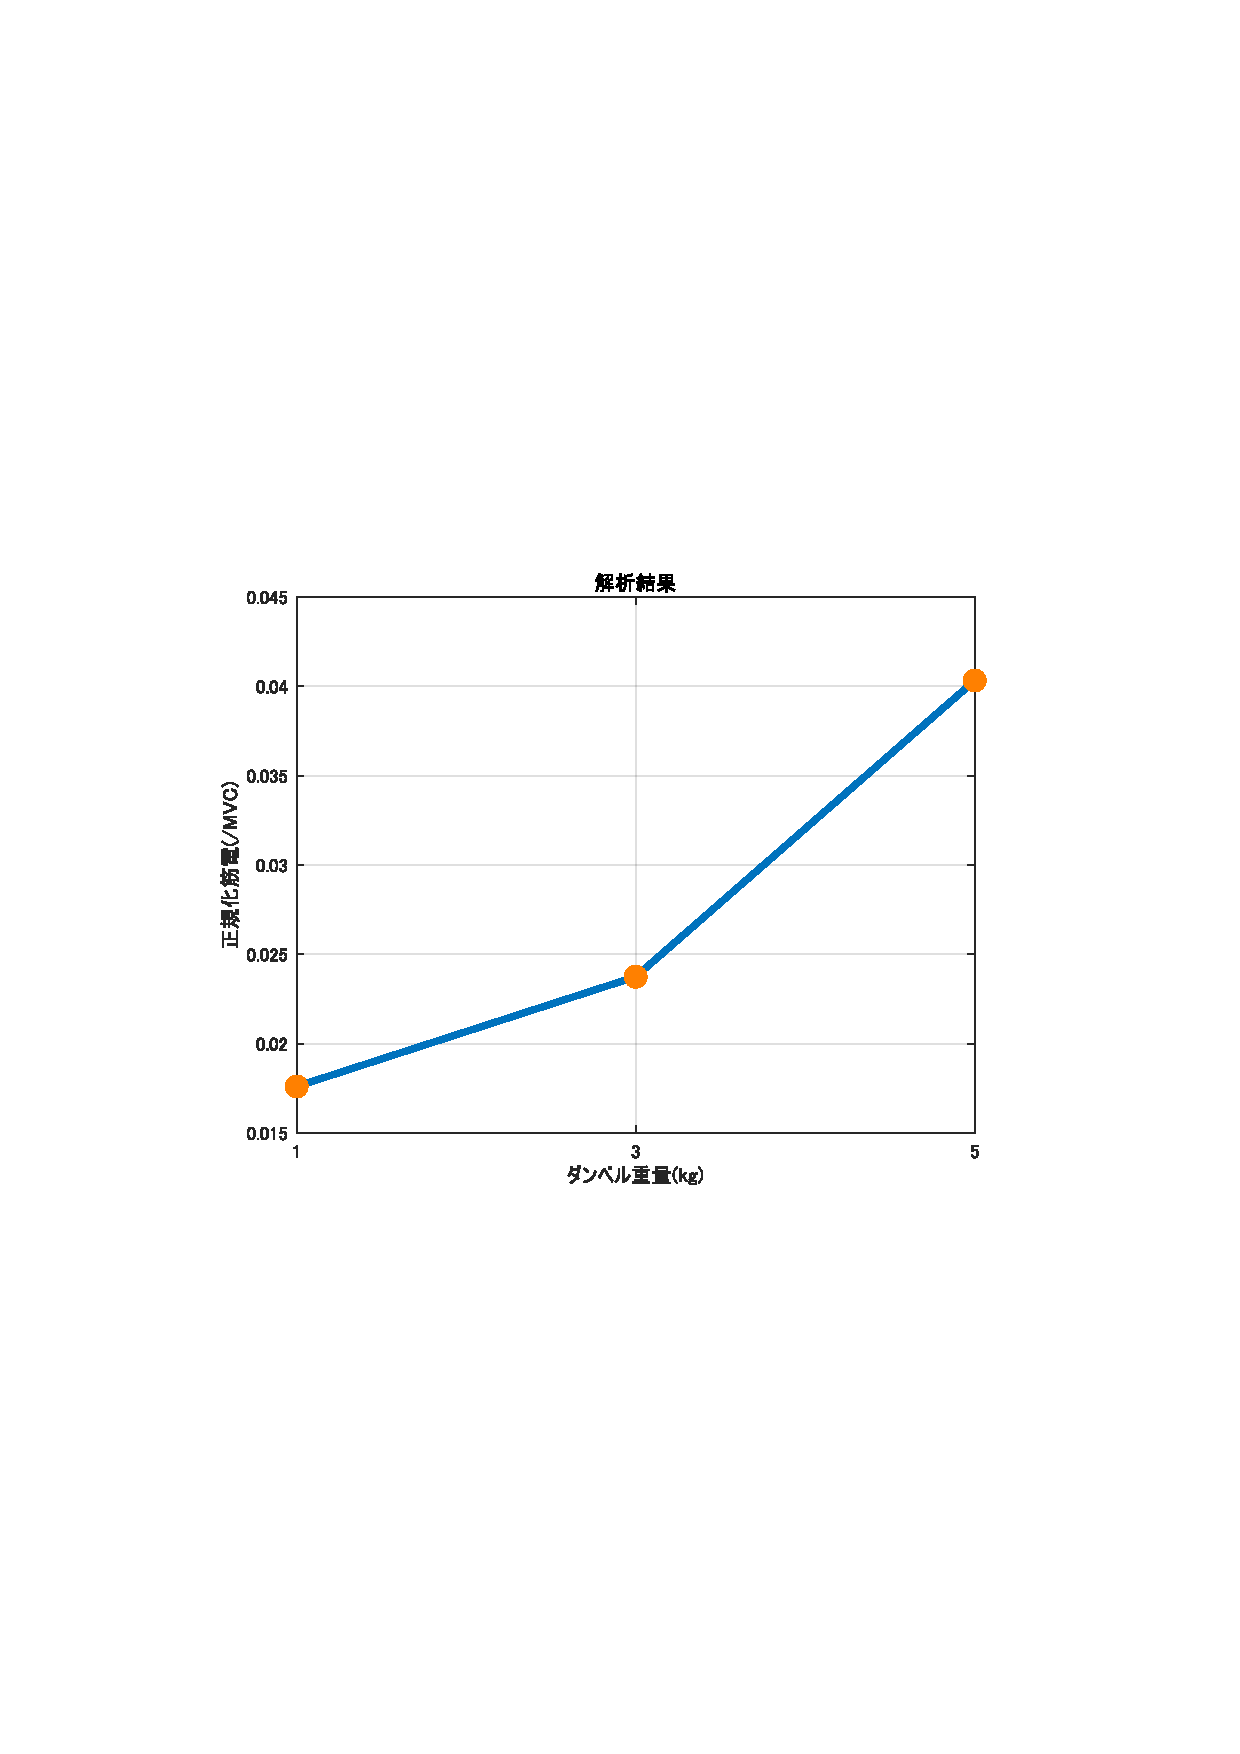
\includegraphics[trim=90 250 100 250 clip,keepaspectratio, width=\linewidth]{figure/norm_all.pdf}
        \caption{解析結果を示すグラフ}
        \label{fig:norm_all}
    \end{figure}

    \section{各回の結果}

    \subsection{第六回の結果}
    第六回では,恒星運動についてのグラフを求めることができた.それが 図\ref{fig:six_ans}である.これから読み取れることは, 655nm から 660nm の間で各スペクトルが急激に谷になっていることがわかる.この吸収線は水素原子の水素アルファ線であると考えることができるため,赤い光が主に吸収されていると思われる.また,それぞれのスペクトルは基線のレベルが異なっており,これは天体の明るさや観測の条件の違いを反映していると考えられる.

        \begin{figure}[H]
        \centering
        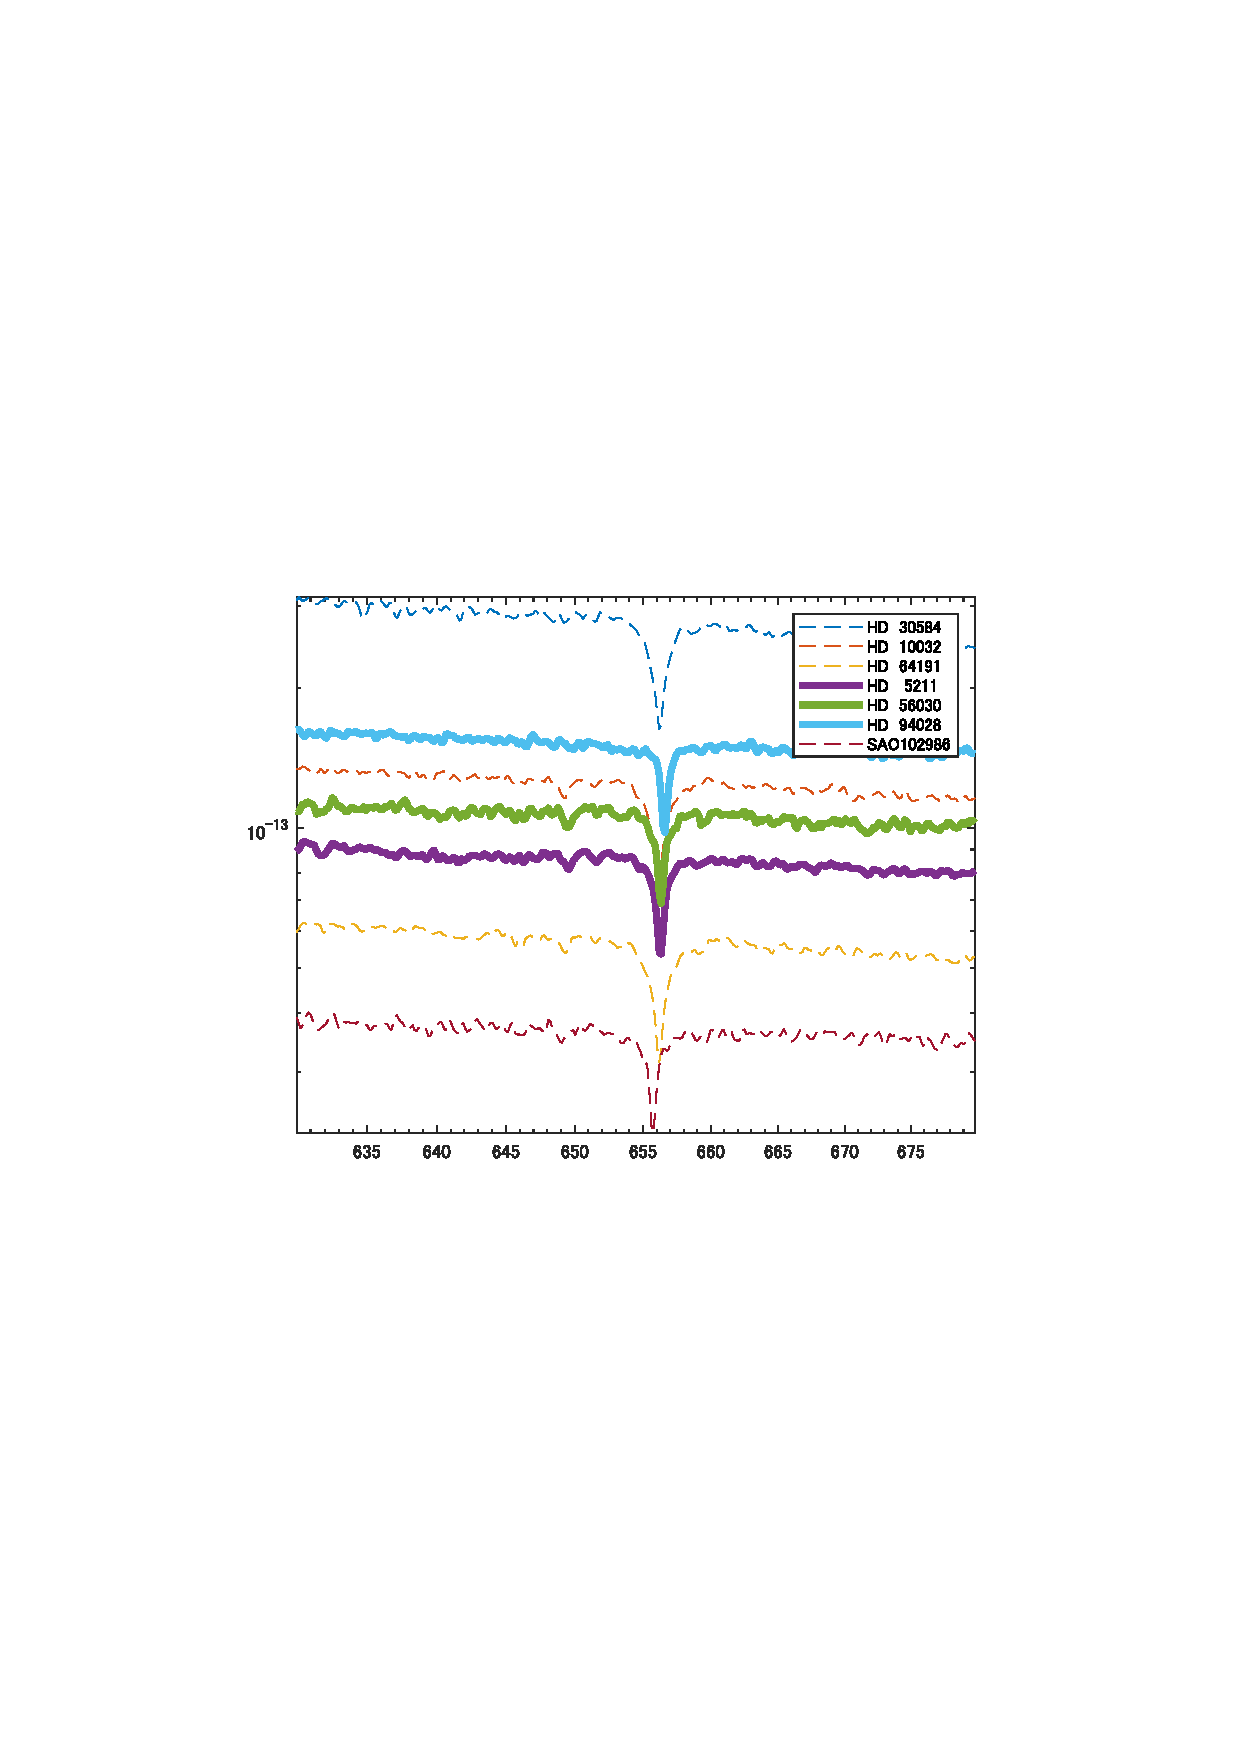
\includegraphics[width=0.5\textwidth]{figure/stellar2.pdf}
        \caption{\ref{fig:exp3_6_spectra2}の再掲}
        \label{fig:six_ans}
    \end{figure}

    \subsection{第七回の結果}
    第七回では眼球運動計測実験で使用するプログラムを作成し,期待通りに動作した.このプログラムを実行した後に書き出される csv ファイルには 1 列目に 試行番号, 2 列目に 被験者が押したキーに対応するキーコード, 3 列目に反応時間が入力される.

    \subsection{第八回の結果}
    

    \subsubsection{眼球運動計測(1)}
        各試行のサッカードの軌跡,速度,潜時などの精密な眼球運動データから顔画像の魅力判断プロセスにおける注意の配分,情報収集のパターンなどが明らかにすることができる.今度は,最終的に選択された画像への注視時間の長さや,特定の顔パーツへの注視頻度等が可能である.

    \subsubsection{眼球運動計測(2)}
        Gaze Plot では,観察対象上に視線の軌跡と固視点を重ねて表示し,被験者がどの順序でどの部分に注目しているのかを視覚的に見ることができる.その結果を 図\ref{fig:gaze} で示す.HeatMapでは,注視が集中した領域を色の濃淡で表現し,対象物の中で特に注意を引いた箇所を直感的に示した図を出力することができる.この結果は 図\ref{fig:heat} である.

        \begin{figure}[H]
            \centering
            \begin{minipage}[b]{0.48\linewidth}
                \centering
                \includegraphics[keepaspectratio, width=\linewidth]{figure/gazeplot1.png}
            \end{minipage}
            \begin{minipage}[b]{0.48\linewidth}
                \centering
                \includegraphics[keepaspectratio, width=\linewidth]{figure/gazeplot2.png}
            \end{minipage}
            \caption{GazePlot の結果}
            \label{fig:gaze}
        \end{figure}

               \begin{figure}[H]
            \centering
            \begin{minipage}[b]{0.48\linewidth}
                \centering
                \includegraphics[keepaspectratio, width=\linewidth]{figure/heatmap1.png}
            \end{minipage}
            \begin{minipage}[b]{0.48\linewidth}
                \centering
                \includegraphics[keepaspectratio, width=\linewidth]{figure/heatmap2.png}
            \end{minipage}
            \caption{Heat Map の結果}
            \label{fig:heat}
        \end{figure}
        
    \subsubsection{脳波計測}
        脳波計測の実験において図 \ref{fig:label} を得た.

        \begin{figure}[H]
            \centering
            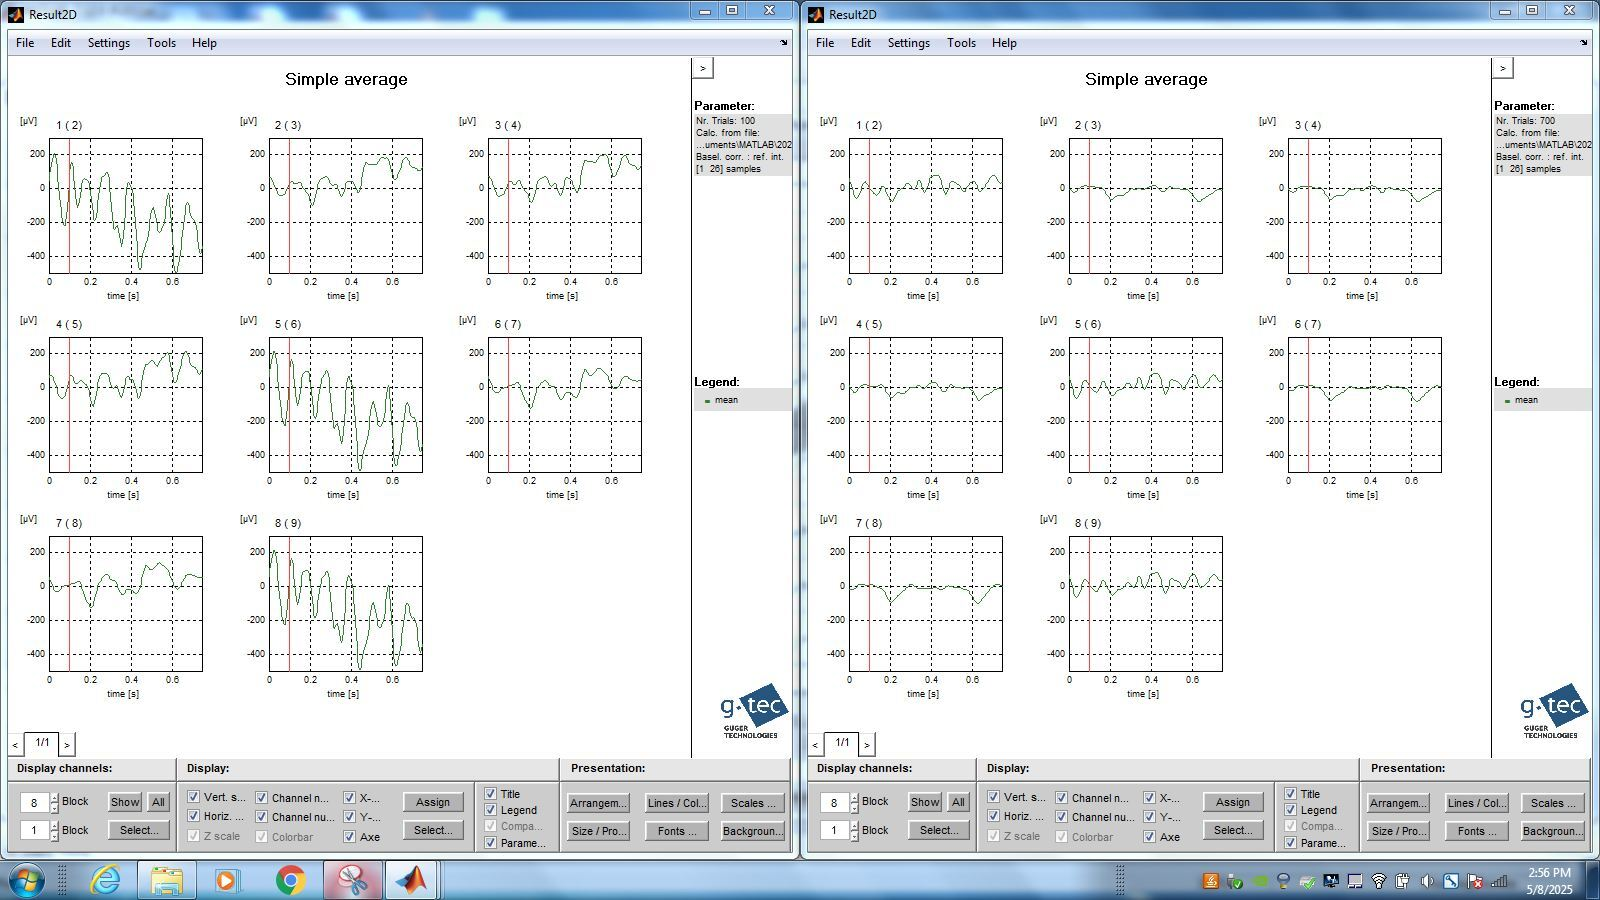
\includegraphics[keepaspectratio, width=0.7\linewidth]{figure/2025-5-6.JPG}
            \caption{脳波実験の結果}
            \label{fig:label}
        \end{figure}

    \subsubsection{筋電計測}
        この実験により, MVC と 1kg, 3kg, 5kg の各ダンベルの負荷時における生の筋電図波形データを得ることができた.図\ref{fig:my_ans} が実際にとれたデータをグラフで表示したものである.これらの図から見たら負荷の増加に伴い筋活動も増加する傾向が見られた.

\begin{figure}[H] % [htbp] は図の配置の優先順位
    \centering % 全体の図を中央揃えにする

    % --- 上段の2つの図 ---
    \begin{subfigure}[b]{0.48\linewidth} % ページの幅の約48%を各図に割り当てる
        \centering
        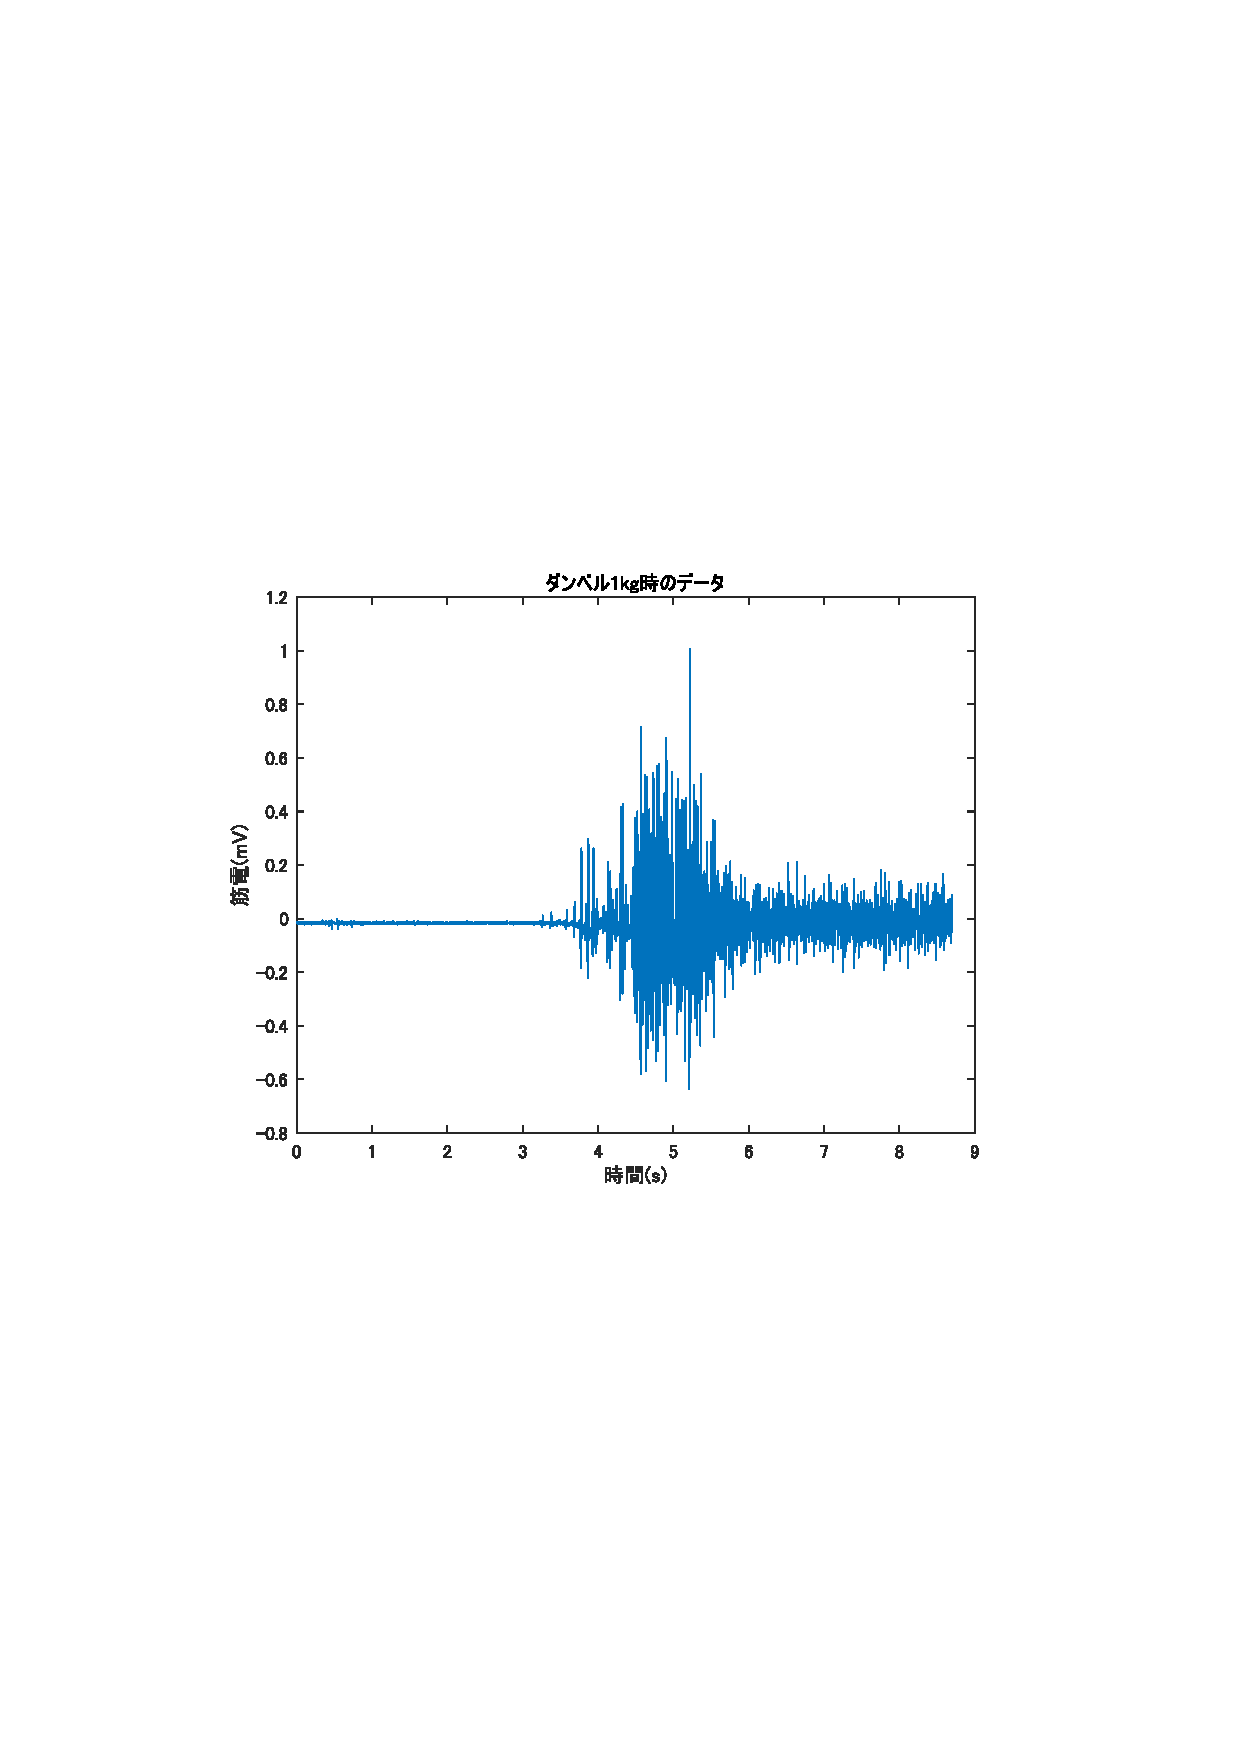
\includegraphics[trim=90 250 100 250 clip,width=\linewidth]{figure/data_1kg.pdf} % サブfigureの幅に合わせて画像を調整
        \caption{MVCの時のデータ} % (a) と表示される
    \end{subfigure}
    \hfill % 残りの水平方向のスペースを均等に埋める
    \begin{subfigure}[b]{0.48\linewidth}
        \centering
        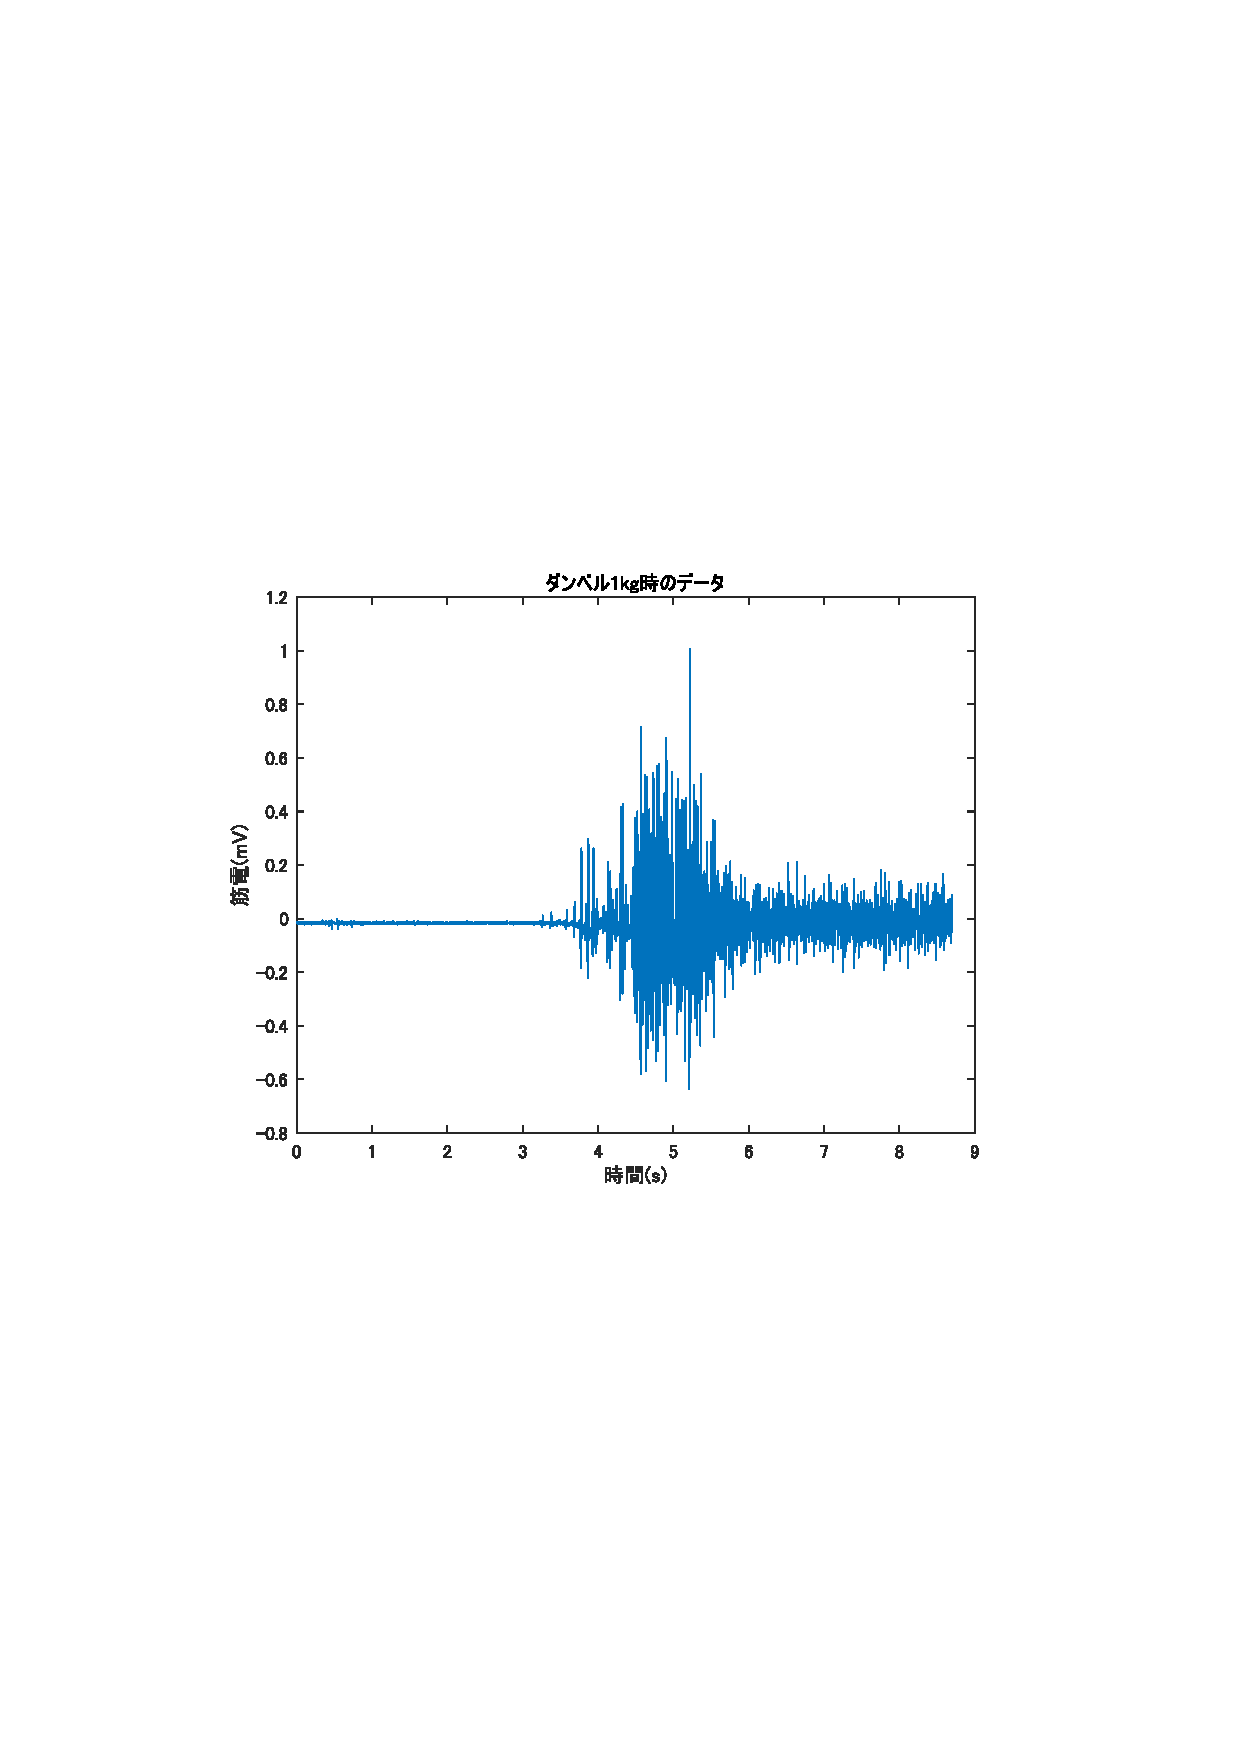
\includegraphics[trim=90 250 100 250 clip,width=\linewidth]{figure/data_1kg.pdf}
        \caption{ダンベルが1kgの時のデータ} % (b) と表示される
    \end{subfigure}

    \vspace{1em} % 上段と下段の間に少し垂直方向のスペースを入れる (任意)

    % --- 下段の2つの図 ---
    \begin{subfigure}[b]{0.48\linewidth}
        \centering
        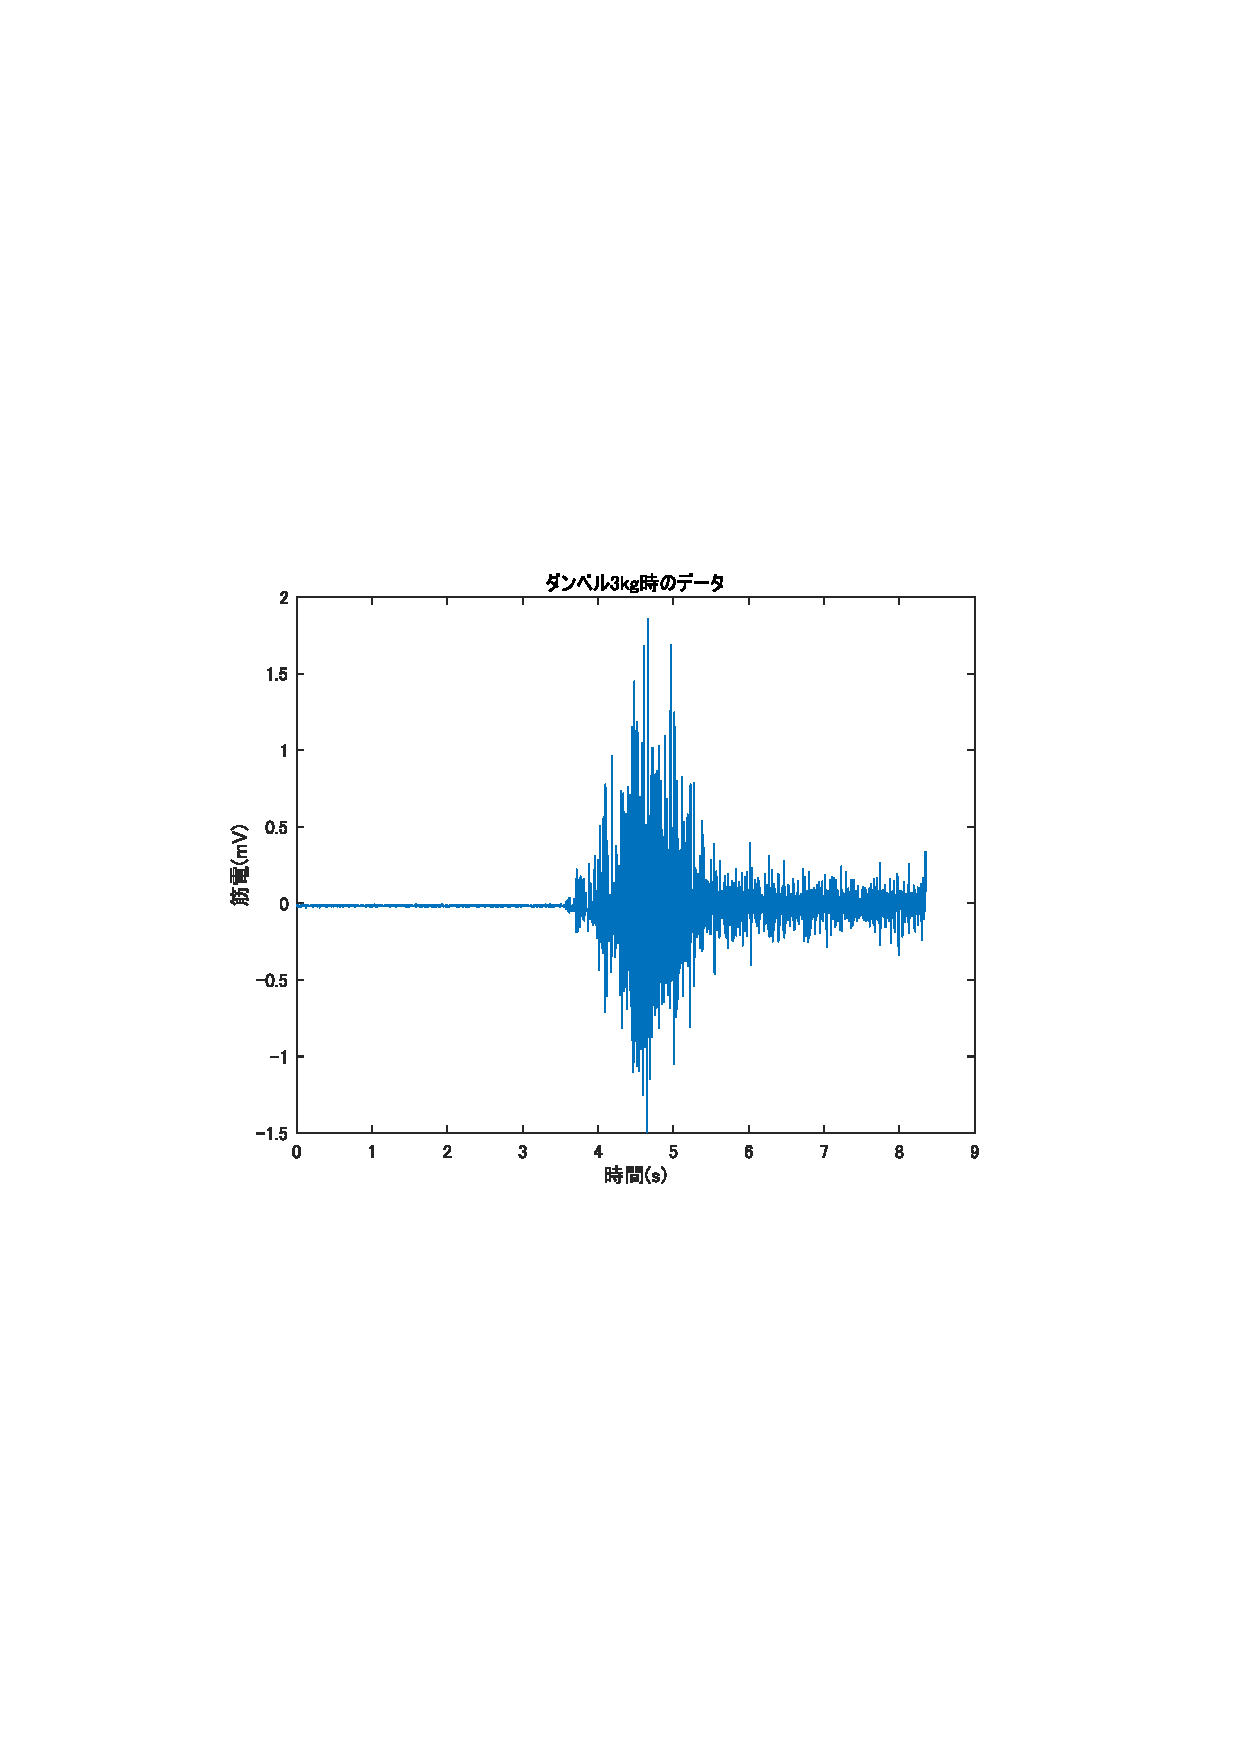
\includegraphics[trim=90 250 100 250 clip,width=\linewidth]{figure/data_3kg.pdf}
        \caption{ダンベルが3kgの時のデータ} % (c) と表示される
    \end{subfigure}
    \hfill
    \begin{subfigure}[b]{0.48\linewidth}
        \centering
        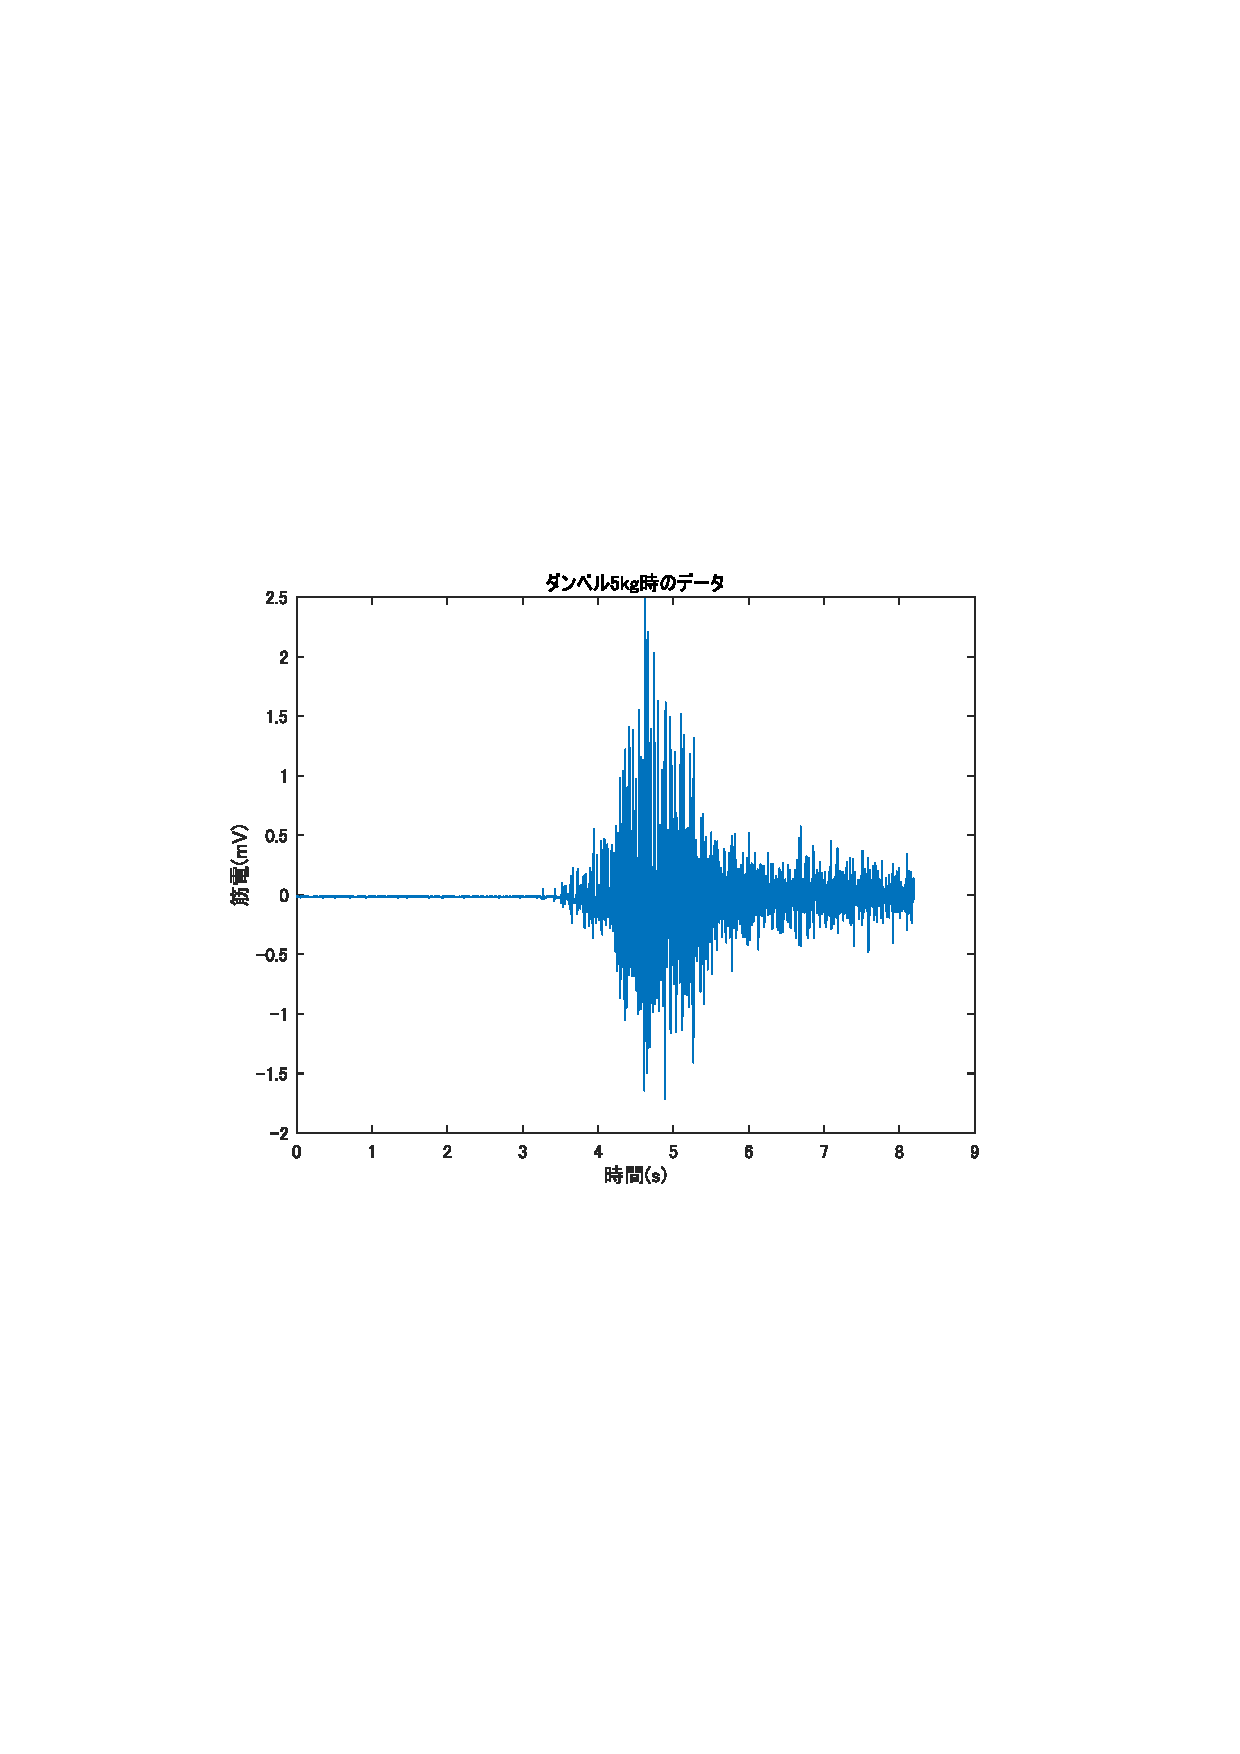
\includegraphics[trim=90 250 100 250 clip,width=\linewidth]{figure/data_5kg.pdf}
        \caption{ダンベルが5kgの時のデータ} % (d) と表示される
    \end{subfigure}

    \caption{図\ref{fig:all_four_images}の再掲} % 図全体に対するキャプション
    \label{fig:my_ans}
\end{figure}        
    

    \subsection{第九回の結果}
    これらの結果より,図\ref{fig:exp3_9_plot} を得ることができる.この図から読み取れることは,-1000ms 付近では割合は比較的低く,どちらかの画像を注視しているかが明確でないか選択していない画像を注視している可能性がある.時間が 0ms に近づくにつれ割合が高くなっており魅力的な画像を注視していることがわかる.また,-500ms, -300ms あたりでは割合が高くなっていることがわかる.最後の 0ms 付近では非常に高い割合に達しいることが分かる.まとめとして,被験者が顔画像の魅力を判断し,キーを教えて選択するまでの最後の 1 秒間で意思決定が固まるにつれ,最終的に選択する画像に対する注視が高まっていく過程を数値化している.
    \begin{figure}[H]
        \centering
        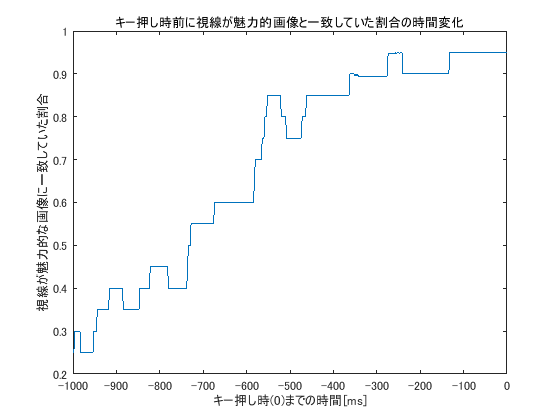
\includegraphics[width=0.5\textwidth]{figure/g0310/lab3_2.png}
        \caption{注視位置と選択位置の一致率}
        \label{fig:exp3_9_plot}
    \end{figure}

    \subsection{第十回の結果}
    第十回の結果として,MVC と及び各ダンベル負荷保持時の筋電図波形がそれぞれのグラフに出力される.それが図\ref{fig:ten_ans}となる.

    \begin{figure}[H]
        \centering
        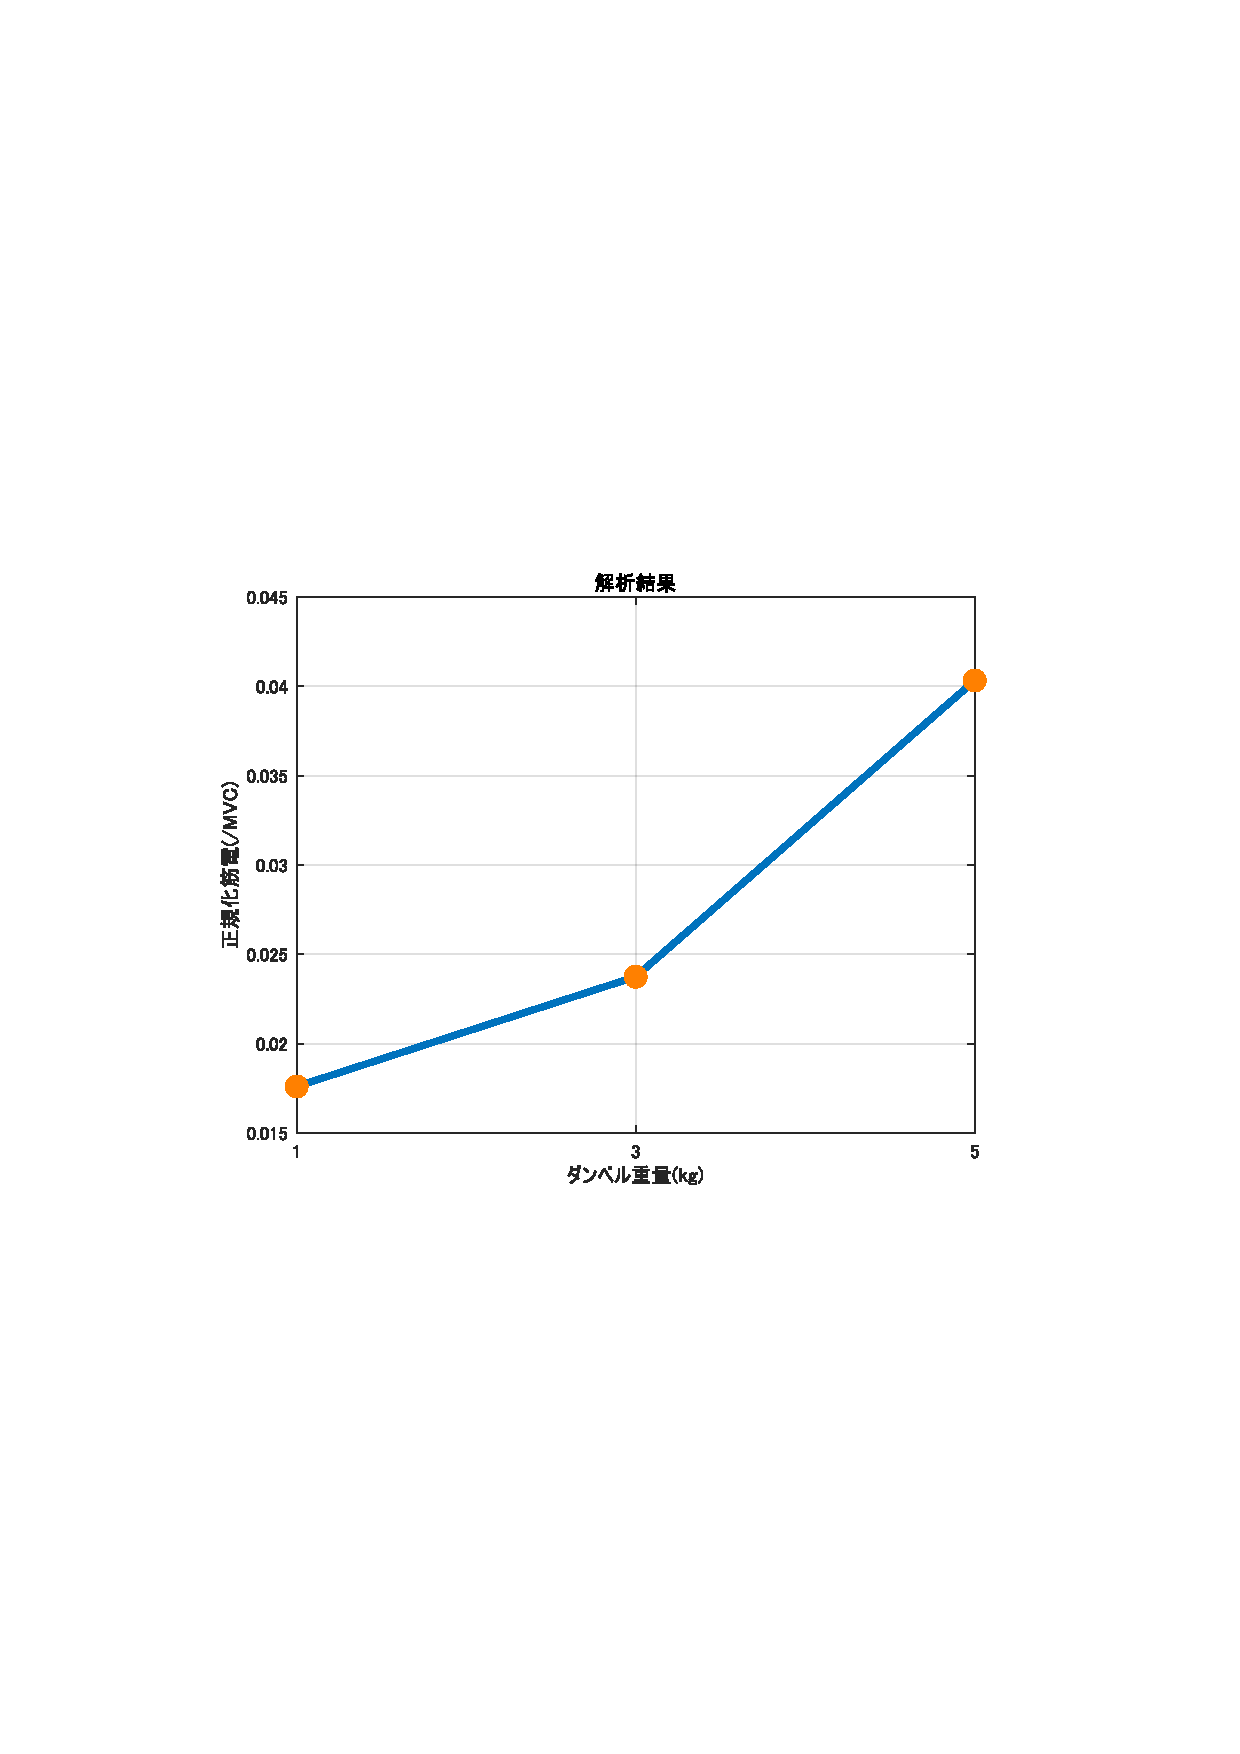
\includegraphics[trim=90 250 100 250 clip,keepaspectratio, width=\linewidth]{figure/norm_all.pdf}
        \caption{\ref{fig:norm_all}の再掲}
        \label{fig:ten_ans}
    \end{figure}

    \section{各回の考察}
    \subsection{第六回の考察}
    図\ref{fig:six_ans} では,この吸収線は水素原子の水素アルファ線であると考えることができるため,赤い光が主に吸収されていると思われる.また,それぞれのスペクトルは基線のレベルが異なっており,これは天体の明るさや観測の条件の違いを反映していると考えられる.

    \subsection{第七回の考察}
    コード\ref{lst:seven_source} を用いることで被験者が魅力的だと判断した顔と注視していた顔の時間変化についてのデータを取ることがで期待できる.

    \subsection{第八回の考察}
    \subsubsection{眼球運動計測実験(2)}
        Tobii Glass 3 での実験では,頭部の動きによる視界の変化やキャリブレーションの意地が難しいという側面があり,今回得られた結果がどの程度正しいのかを考える必要があると思われrう.また,注視している内容についてどのように一般化できるのかについても考えていきたい.

    \subsubsection{筋電計測}
    ダンベル重量の増加に伴う正規化筋電位の変化パターンが,筋の動員特性等とどのような関連であるかを筋電計測の解析で明らかにしていきたいと考えた.

    \subsubsection{脳波計測}
    今回は,一人を対象とした実験であったため個人差を埋めることができないと考えられる.したがって,今回と同様の実験を行うことで個人差を埋め,より安定的な結果を得たい.
    
    \subsection{第九回の考察}
    実験の開始時の -1000ms 付近では一致率が0.2程度と低かったが時間が経つほどに割合が増え,最終的には0.9以上の割合だったため,時間が経つほどに被験者の視線はほぼ魅力的だと判断した画像に向けられていることを意味していると考えられる.
    
    \subsection{第十回の考察}
    図\ref{} から,負荷が高くなるほど,筋電位が高くなっており,より多くの運動単位が動員され,発火頻度も増えるため,筋電図の振幅は増大していることがわかった.重すぎるものを持ち上げることができない場合と今回測定した MVC では筋電図が同じになるのかについて疑問が残ったため,検証していきたいと思った.
    \section{総合結論}
        これらの実験を通して,眼球運動,筋電,脳波等の計測方法や実験の手法に加えて Matlab の使用方法についても学ことができた.眼球運動計測実験では, EyeLink II を用いた魅力的な顔画像の判断課題で視線行動の記録・分析や解析方法及び Tobii Glass 3 を用いたポスターを見たい自然な状況下を想定した注視の可視化を行った.この内容は,現代の広告にも活かすことができると聞き,これからの社会におけるデータ収集,分析等の必要性について改めて確認することができた.また,筋電計測実験では,上腕二頭筋の筋活動を最大随意収縮を基準とし, 1kg, 3kg, 5kg の異なるダンベル負荷の記録・解析を行った.ベースライン補正,全波整流,正規化,フィルタリングといった処理を通じてそれぞれどのような役割を担っているのかを理解することができた.脳波計測実験では, P300 を指標とするブレイン・マシン・インタフェースで視覚刺激を用いて脳波からタイピングを行うことを体験し,脳情報を外部機器に対しての制御に用いる手法について学んだ.このような経験は,人間の仕組みを理解し応用するための方法とその実践方法について学べたと考える.
    \appendix
    
    \section{第六回で作成したソースコード}  
   \definecolor{bg}{rgb}{0.95,0.95,0.95}
    \begin{mdframed}[
        splitbottomskip=10pt, splittopskip=10pt,         
        backgroundcolor=bg,
        topline=false,
        bottomline=false,
        leftline=false,
        rightline=false]
        \inputminted[linenos, 
        frame=lines, 
        breakanywhere=true,
        breaklines,
        fontsize=\small]{matlab}{code/Exp3_6_Matlab.m}    
    \end{mdframed}
    \captionof{listing}{HD94028の運動についてのグラフを出力を行うプログラム}

    \definecolor{bg}{rgb}{0.95,0.95,0.95}
    \begin{mdframed}[
        splitbottomskip=10pt, splittopskip=10pt,         
        backgroundcolor=bg,
        topline=false,
        bottomline=false,
        leftline=false,
        rightline=false]
        \inputminted[linenos, 
        frame=lines, 
        breaklines,
        breakanywhere=true,
        fontsize=\small]{matlab}{code/Exp3_6_2_Matlab.m}    
    \end{mdframed}
    \captionof{listing}{複数の恒星運動についてのグラフを出力を行うプログラム}    

    \newpage
    \section{第七回で作成したソースコード}
    \definecolor{bg}{rgb}{0.95,0.95,0.95}
    \begin{mdframed}[
        splitbottomskip=10pt, splittopskip=10pt,         
        backgroundcolor=bg,
        topline=false,
        bottomline=false,
        leftline=false,
        rightline=false]
        \inputminted[linenos, 
        frame=lines, 
        breakanywhere=true,
        breaklines,
        fontsize=\small]{matlab}{code/Exp3_7_Matlab.m}    
    \end{mdframed}
    \captionof{listing}{第八回で行われる予定だった眼球運動計測実験(1)を解析するプログラム}
    
    \newpage
    \section{第九回で作成したソースコード}
    \definecolor{bg}{rgb}{0.95,0.95,0.95}
    \begin{mdframed}[
        splitbottomskip=10pt, splittopskip=10pt,         
        backgroundcolor=bg,
        topline=false,
        bottomline=false,
        leftline=false,
        rightline=false]
        \inputminted[linenos, 
        frame=lines, 
        breakanywhere=true,
        breaklines,
        fontsize=\small]{matlab}{code/Exp3_9_Matlab.m}    
    \end{mdframed}
    \captionof{listing}{第八回で行われる予定だった眼球運動計測実験(1)を解析するプログラム}

    \newpage

    \section{第十回で作成したソースコード}
    \definecolor{bg}{rgb}{0.95,0.95,0.95}
    \begin{mdframed}[
        splitbottomskip=10pt, splittopskip=10pt,         
        backgroundcolor=bg,
        topline=false,
        bottomline=false,
        leftline=false,
        rightline=false]
        \inputminted[linenos, 
        frame=lines, 
        breakanywhere=true,
        breaklines,
        fontsize=\small]{matlab}{code/Exp3_10_Matlab.m}    
    \end{mdframed}
    \captionof{listing}{筋電計測のデータを計測するプログラム}


\begin{thebibliography}{99} % {99} の部分は後述

  \bibitem{}
    カンデル神経科学,宮下保司,メディカルサイエンスインターナショナル, 2022/9/30
  \bibitem{}
  PC と USB 接続カメラを用いた眼球運動計測, 十河宏行,  \url{https://www.jstage.jst.go.jp/article/pacjpa/76/0/76_2PMA35/_pdf} 参照日 : 2025年05月28日
  \bibitem{}
    優柔不断な選択者を後押しする眼鏡型デバイスの実現とその評価, 小松原達哉, \url{https://dl.nkmr-lab.org/papers/396/paper.pdf} 参照日 : 2025年05日28日
  \bibitem{}
  筋電操作ハンドの制御のための皮膚表面筋電信号のニューラルネットによる認識, 平岩明, \url{https://www.jstage.jst.go.jp/article/sicetr1965/30/2/30_2_216/_pdf} 参照日 : 2025年05月28日
  \bibitem
  ボーカルアレンジが楽曲の好みに及ぼす影響と脳波特性の関係, ライ モウテイ, \url{https://chuo-u.repo.nii.ac.jp/record/15084/files/nenpou19N7100021K.pdf}
  % さらに文献が続く場合は同様に記述

\end{thebibliography}
    
\end{document}